\chapter{Estimation des coûts de production par apprentissage}
\minitoc
\newpage
\label{neurones}
\section{Introduction}
\begin{table}[H]
	\centering
	\begin{tabular}{|*{2}{m{8cm}|}}
		\hline
		\rowcolor{cyan}	Noms & Définitions\\
		\hline
		Itérations & Nombre de fois que l'ensemble des données sera passé au réseau de neurones lors de la phase d'entrainement\\
		\hline
		Batch & Nombre d'échantillons qui passeront par le réseau de neurones à chaque cycle d'apprentissage\\
		\hline
		Cycle d'apprentissage &  Un nouveau cycle d'apprentissage commence à chaque fois que les poids synaptiques du réseau sont recalculés\\
		\hline
		
	\end{tabular}
	\caption[Glossaire]{Glossaire. \label{gloss}}
\end{table}
 
 
Dans ce chapitre, on cherche à construire un outil d'aide à la décision basé sur les réseaux de neurones qui pourra estimer rapidement le coût de production associé à une stratégie de recharge réduite décrite à la section (\ref{recharge_reduite}) du chapitre précédent. Autrement dit, on construit donc ici un estimateur rapide des coûts de production.
Cet outil pourrait servir à aider un décideur à prendre des décisions sur des stratégies de recharge réduite afin de limiter les risques de perte (de temps ou d'argent). Par exemple le décideur pourrait avoir plusieurs stratégies de recharge réduite et voudrait décider rapidement quelle stratégie réaliser.

 Cet estimateur pourrait aussi par exemple servir à optimiser la tournée du véhicule. Dans les chapitres précédents, on a présenté plusieurs méthodes de résolution du problème SMEPC. On a notamment présenté au chapitre \ref{Heuristique} un schéma collaboratif nommé Pipe-line VD\_PM car il a été constaté que le problème SMEPC peut être divisé en deux sous-problèmes à savoir le problème \textit{Vehicle-Driver} et le problème de production \textit{Production-Manager}. Il ressort de nos expérimentations numériques que parmi les deux algorithmes de résolution des deux sous-problèmes, celui qui est lourd en temps CPU est l'algorithme de résolution du problème \textit{Production-Manager}.
Dans les chapitres précédents, on a fixé la tournée du véhicule, autrement dit on a supposé qu'on connait dans quel ordre les stations seront visitées car notre objectif était de se focaliser uniquement sur les aspects synchronisation du problème SMEPC. L'outil d'aide à la décision construit dans ce chapitre pourrait être utilisé pour optimiser la tournée du véhicule. Pour évaluer le coût de production, on pourrait bien évidemment utiliser le module PM de Pipe-line VD\_PM mais ce module étant lourd en temps CPU, on veut construire un réseau plus rapide qui peut remplacer ce module et évaluer le coût de la partie production PM.  Pour cela, on peut utiliser cet outil pour obtenir une approximations de la qualité d'une tournée très rapidement.

Les entrées du modèle SMEPC que nous utiliserons pour construire nos réseaux de neurones pour le problème de production sont présentées au tableau (\ref{inputs_learn}).
\begin{table}[H]
	\centering
	\begin{tabular}{|*{2}{m{8cm}|}}
		\hline
		\rowcolor{cyan}	Noms & Significations\\
		\hline
		$C^{Tank}$ & Capacité de la citerne d'hydrogène\\
		\hline
		$C^{Veh}$  & Capacité du réservoir d'hydrogène du véhicule   \\
		\hline
		$N$  & Nombre de périodes de production    \\
		 \hline
		$H_0$  & Charge initiale de la citerne d'hydrogène \\
		\hline
		$Cost^F$  & Coût d'activation de la micro-usine \\
		\hline
		Pour $i=0, \dots, N-1$, $R_i$ &Rendement de production lié à la période $i$ \\
		\hline
		Pour $i=0, \dots, N-1$, $Cost_i^V$ &  Coût de production lié à la période $i$ \\
		\hline
		$Q$ & Nombre d'opérations de recharge en carburant effectuées par le véhicule \\
		\hline
		Pour $q=1, \dots, Q$, $\mu_q$ & Quantité d'hydrogène qui est rechargée lors de la $q^{i\grave eme}$ opération de recharge \\
		\hline
		Pour $q=1, \dots, Q$, $[m_q,M_q]$ & Fenêtre de temps de la $q^{i\grave eme}$ opération de recharge \\
		\hline
	\end{tabular}
	\caption[Entrées utilisées pour construire nos réseaux de neurones ]{Entrées utilisées pour construire nos réseaux de neurones. \label{inputs_learn}}
\end{table}

Les schémas d'apprentissage que nous avons choisi d'explorer ici sont les réseaux de neurones.
Il existe plusieurs types de réseaux de neurones. Ces réseaux de neurones se différencient par la manière dont les informations sont propagées entre les différentes couches de neurones. La variante la plus simple est celle du réseau de neurones dit  \textit{ feed-forward}, ici, les informations passent directement de la couche d'entrée aux couches cachées puis à la couche de sortie. Dans ce chapitre, on s'intéresse uniquement  à ce type de réseau de neurones et la fonction d'agrégation utilisée est la somme pondérée. Mais il existe d'autres types de réseaux de neurones à savoir les réseaux de neurones récurrents et les réseaux de neurones convolutifs. Les réseaux de neurones récurrents sauvegardent les résultats produits par les neurones et nourrissent le réseau à l'aide de ces résultats. Ce mode d'apprentissage est un peu plus complexe.
Les réseaux de neurones convolutifs sont quant à eux de plus en plus utilisés dans différents domaines : reconnaissance d'images, traitement naturel du langage. En reconnaissance d'images par exemple, un réseau de neurones convolutifs est constitué de deux parties : une première partie dite convolutive qui est chargée de faire la compression (réduction de la dimension) des images et une deuxième partie classification du réseau qui correspond à un réseau Perceptron Multicouche dont l'acronyme est MLP (\textit{Multi Layers Perceptron}). Un MLP est un réseau à propagation \textit{ feed-forward} constitué de plusieurs couches. 

Le nombre de données d'entrée et les données de sortie du réseau de neurones sont généralement fixés par la nature du problème. 
Le nombre de couches cachées et le nombre de neurones par couche n'est pas facile à déterminer, cela dépend principalement de la quantité et de la complexité des données. En général, quand on augmente le nombre de neurones cachés, on gagne de la
précision sur les données utilisées en apprentissage mais le réseau perd sur son pouvoir de généralisation pour d'autres données, d'où l'expression sur-apprentissage. Ainsi, plus le nombre de couches et de neurones est élevé, plus le réseau aura besoin d'une grande quantité de données pour être entrainé efficacement. Une architecture qui donne de bons résultats pour une application donnée ne peut être déterminée que d'une façon expérimentale. Pour construire un réseau de neurones, on a besoin de fixer un certain nombre de paramètres. Parmi eux, on peut citer la fonction d'activation, le nombre d'itérations (appelé epochs dans le vocabulaire des réseaux de neurones) et la taille du batch.
La fonction d'activation permet de normaliser les sorties de neurones dans un intervalle prédéfini. Par exemple, les sorties de neurones peuvent être échelonnées sur un intervalle [0,1] par la fonction sigmoïde : ${\displaystyle f(x)={\frac {1}{1+{\rm {e}}^{-x}}}}$.
 Le nombre d'itérations représente le nombre de fois que l'ensemble des données sera passé au réseau de neurones lors de la phase d'entrainement. Plus le nombre d'itérations est grand, plus le réseau sera entrainé longtemps. %ce qui donnera également de meilleurs résultats.
  La taille du batch représente le nombre d'échantillons qui passeront par le réseau de neurones à chaque cycle d'apprentissage. Un nouveau cycle d'apprentissage commence à chaque fois que les poids synaptiques du réseau sont recalculés.

Au début de la phase d'apprentissage, les données d'apprentissage et de validation sont présentées au réseau avec la valeur de sortie (le cout de production) correspondantes. Les valeurs des poids sont ajustées et affinées continuellement tout au long de la phase d'apprentissage. La correction des poids au cours de l'entraînement ne tient compte que des données d'apprentissage. Au cours de cette phase, les poids du réseau sont corrigés de manière à minimiser l'erreur au carré entre la réponse calculée par le réseau et la réponse attendue. Généralement, l'erreur calculée sur les données d'apprentissage diminue continuellement au cours de l'entraînement. Toutefois, une longue phase d'entraînement diminue la capacité de généralisation du réseau en l'adaptant uniquement aux données d'apprentissage. À cet effet, les données de validation déterminent à quel moment l'apprentissage doit être arrêté. Les données de validation représente généralement 1/3 des données d'apprentissage. Les données de validation servent uniquement à vérifier le comportement du réseau au cours de l'entraînement face à des données qui lui sont étrangères.
Généralement, contrairement à l'erreur calculée sur les données d'apprentissage qui diminue continuellement au cours de l'entraînement, celle calculée sur les données de validation diminue dans la première phase d'entraînement en suivant une allure semblable à celle des données d'apprentissage avant de commencer une lente ascension. Ceci est expliqué par le fait que le réseau commence à perdre son pouvoir de généralisation en adaptant les poids de ses neurones uniquement aux données d'apprentissage. L'entraînement du réseau sera donc arrêté dès que cette erreur commence son ascension. Toutefois, afin d'éviter un arrêt prématuré d'apprentissage causé par une augmentation ponctuelle de l'erreur des données de validation, on introduit souvent un seuil de décision qui tolère des légères ascensions successives de l'erreur. Si l'erreur sur les données de validation continue son ascension au delà de ce seuil, on arrête l'apprentissage du réseau et on conserve les valeurs des poids qui correspondent à l'itération qui précède cette ascension.

Après l'arrêt de la phase d'apprentissage, on vérifie la performance du réseau avec les données de test. Ces données n'ont pas servi à l'apprentissage et n'ont joué aucun rôle dans la prise de décision dans l'arrêt de l'apprentissage. Les données de test sont utilisées uniquement pour mesurer la performance du réseau après l'arrêt de l'apprentissage. Si le réseau arrive à faire des prédictions correctes avec un gap acceptable, on peut dire que le réseau est opérationnel. Dans le cas contraire, il faut réviser le réseau et recommencer l'apprentissage. 

Dans la \textbf{section} \ref{seq_funct}, on présente trois réseaux de neurones : \textbf{SIMPLE\_TYPE}, \textbf{SIMPLE\_PERIODE} et \textbf{MIXTE}.
% dont deux réseaux basiques et un réseau sophistiqué.
 Les réseaux \textbf{SIMPLE\_TYPE} et \textbf{SIMPLE\_PERIODE} prédisent le coût de production.
%, pour faire référence à ces deux réseaux on utilisera le terme \textbf{SIMPLE} puisqu'ils ont exactement le même nombre de couches et de neurones. La seule différence entre eux est la manière dont les données sont agencées avant d'être placées en entrées.
 Le réseau \textbf{MIXTE} contrairement aux réseaux \textbf{SIMPLE\_TYPE} et \textbf{SIMPLE\_PERIODE}, essaye d'épouser les caractéristiques du problème. Le réseau \textbf{MIXTE} prédit le coût de production (on nomme cette partie du réseau \textbf{MIXTE\_COUT}) et le numéro de période de la dernière recharge (on nomme cette partie du réseau \textbf{MIXTE\_TEMPS}). Puisque les données d'entrées des réseaux de neurones \textbf{SIMPLE\_TYPE}, \textbf{SIMPLE\_PERIODE} et \textbf{MIXTE} sont nombreuses cela a pour effet d'augmenter considérablement le nombre de poids. Dans ce chapitre, on va se focaliser uniquement sur des instances à 20 périodes. Pour pallier à ce problème d'augmentation du nombre de poids, on va construire d'autres réseaux de neurones dont les entrées seront des indicateurs. On va définir un ensemble d'indicateurs qui vont représenter nos données de façon plus compacte.
Dans la \textbf{section} \ref{RN_PM}, on commence par présenter les indicateurs qui serviront d'entrée aux réseaux de neurones basés sur les indicateurs. On finit cette section en présentant l'architecture de nos réseaux de neurones basés sur les indicateurs qu'on nomme \textbf{INDIC\_TEMPS} et \textbf{INDIC\_COUT} qui font respectivement une approximation  du numéro de période de la dernière recharge et du coût de production. Dans la \textbf{section} \ref{RN_exp}, on montre les résultats des expérimentations numériques de tous les réseaux de neurones. On présente au préalable les instances qui ont été utilisées pour entrainer les réseaux. Pour simplifier le problème, on ne travaille qu'avec des instances qui ont le même nombre de périodes.

\section{Réseaux de neurones dont les entrées sont des données brutes}
\label{seq_funct}

Cette section présente la méthodologie suivie pour la conception et l'apprentissage des réseaux de neurones pour la prédiction du coût de production correspondant à une stratégie de recharge réduite. Plus précisément, on décrit deux réseaux qu'on nomme \textbf{SIMPLE\_TYPE} et \textbf{SIMPLE\_PERIODE} et un réseau qu'on nomme \textbf{MIXTE} en définissant les éléments suivants : le format des données d'entrées, l'architecture des réseaux de neurones, les fonctions d'activation et l'algorithme d'apprentissage. Les réseaux de neurones de cette section ont été implémenté en python à l'aide de Keras qui dispose de plusieurs modules de création et d'entrainement de réseaux de neurones.

Tout au long de ce chapitre, nous utiliserons les expressions suivantes :
\begin{itemize}[label=$\square$]
	\item \textit{Layer Dense} correspond à des couches dont les neurones reçoivent en entrée une valeur égale à la somme pondérée de l'ensemble des neurones de la couche précédente ;
	\item \textit{Multiply Dense} permet de multiplier la valeur de sortie de 2 couches de neurones terme à terme.
	\item \textit{Layer Concatenate} recopie les neurones de leur couche initiale vers la couche de concaténation sans modification de leur valeur de sortie
\end{itemize}
\subsection{Construction des réseaux \textbf{SIMPLE\_TYPE} et \textbf{SIMPLE\_PERIODE} pour la prédiction du coût de production} 
Lorsqu'on parle de réseau \textbf{SIMPLE\_} on fait allusion aux deux réseaux nommés \textbf{SIMPLE\_TYPE} et \textbf{SIMPLE\_PERIODE}. Dans cette section, notre objectif est de construire deux réseaux de neurones \og simple \fg{} qui serviront de base pour la comparaison avec les réseaux plus sophistiqués. Concernant les entrées du réseau, nous allons tester deux façons de les agencer qu'on nomme ici agencement par période et par type. Autrement dit, on a classé les données par type (le réseau obtenu s'appelle \textbf{SIMPLE\_TYPE}) et par période (le réseau obtenu s'appelle \textbf{SIMPLE\_PERIODE}). Par exemple, pour une instance de trois périodes, si les données sont : 
\begin{itemize}[label=$\square$]
\item Le coût fixe est $A=[1,1,1]$ ;
\item Le coût variable est $Cost_i^V=[5,5,5]$ ;
\item La date de début de la dernière recharge est 2 ;
\item Le rendement est $R= [10, 10, 10]$ ;
\item La recharge est $Recharge=[0,3,0]$.
\end{itemize}
 Si les données sont classées par \textbf{type} alors elles seront agencées de la façon suivante \og 
 1, 1, 1, 5, 5, 5, 2, 10, 10, 10, 0, 3, 0\fg{}. Si les données sont classées par \textbf{période} alors elles seront agencées de la façon suivante \og 1, 5, 10, 0, 1, 5, 10, 3, 1, 5, 10, 0, 2 \fg{}. Concernant les fonctions d'activation, on va tester plusieurs combinaisons pour voir celles qui fonctionnent le mieux pour notre problème.

%Pour se familiariser avec les réseaux de neurones, on construit les réseaux qu'on nomme \textbf{SIMPLE\_TYPE} et \textbf{SIMPLE\_PERIODE}. %On suppose ici que la sortie qu'on veut calculer est une combinaison linéaire de nos entrées. Ceci étant dit, il est fort probable que le réseau \textbf{SIMPLE} ne fournisse pas de bons résultats, c'est-à-dire ne fasse pas de bonnes approximations.
Dans les réseaux \textbf{SIMPLE\_TYPE} et \textbf{SIMPLE\_PERIODE}, les entrées de chaque couche sont les sorties de la couche précédente. Et chaque neurone de chaque couche est connecté à tous les neurones de la couche précédente.
Dans cette section, on va décrire les données d'entrée, l'architecture et les données de sortie de notre réseau.
%Modèle séquentiel complètement connecté

\subsubsection{Description des entrées des réseaux de neurones \textbf{SIMPLE\_}}
% le format des données d'entrées, l'architecture des réseaux, la fonction d'activation, l'algorithme d'apprentissage, le taux d'apprentissage et les critères d'arrêt d'apprentissage.
%couche,poid,biais, fonction d'activation


Les données utilisées lors de la phase d'entrainement des réseaux de neurones doivent être pertinentes pour la prédiction du coût de production. Dans notre cas, les données d'entrée seront les suivantes :
\begin{itemize}[label=$\square$]
\item  Le coût d'activation $A=A_i$, avec $i \in \{0, \dots, N-1\}$ puisque dans notre problème le coût d'activation est $Cost^F$, on pose ici $\forall i, A_i=Cost^F$, $N$ est le nombre de périodes ;

\item Pour $i=0, \dots, N-1$, $Cost_i^V$ est la coût de production lié à la période $i$ ;
\item Le numéro de période du début de la dernière recharge
\item Pour $i=0, \dots, N-1$, $R_i$ est le rendement de production lié à la période $i$ ;
\item $Q$ est le nombre d'opérations de recharge en carburant effectuées par le véhicule ;
\item $\mu_q$ est la quantité d'hydrogène qui est rechargée lors de la $q^{i\grave eme}$ opération de recharge ;
\item Des bornes inférieures $m_1, \dots,m_Q$ respectivement pour les numéros de période $i_1, \dots, i_Q\in \{0, \dots, N-1\}$ lorsque les opérations de recharge en hydrogène ont lieu ; 

\item  Un vecteur $Recharge$ rempli de la façon suivante : Pour $q=1, \dots, Q$, $\mu_q$ et $i \in [m_q,M_q]$, $Recharge_i=\mu_q$ sinon $Recharge_i=0$. 
%où $\mu_q$ est la quantité d'hydrogène rechargée par le véhicule à la $q^{i\grave eme}$ recharge qui se produit entre la date $m_q$ et la date $M_q$.

\end{itemize}


% \textbf{On considère que la taille de notre réseau est la plus grande valeur de $N$}.
\subsubsection{Description des architectures des réseaux de neurones \textbf{SIMPLE\_}}

Ces réseaux de neurones sont complètement connecté c'est-à-dire que tous les neurones d'une couche sont connectés à tous les neurones de la couche précédente. Dans notre réseau, le nombre de couches et le nombre de neurones des couches a été choisi assez faible pour ne pas avoir trop de poids. %La fonction d'activation utilisée est la fonction linéaire (Elle est la fonction identité).
L'architecture de ces réseaux de neurones que nous avons conçu est la suivante :

\begin{itemize}[label=$\square$]
	\item Elle a une couche d'entrées constituée de huit neurones
\item Elle a une couche cachée constituée de quatre neurones
\item Elle a une couche de sortie constituée d'un neurone
\end{itemize}   

La figure (\ref{SFC}) représente l'architecture du réseau \textbf{SIMPLE\_TYPE}, ici les données sont classées par type. La figure (\ref{SFC2}) représente l'architecture du réseau \textbf{SIMPLE\_PERIODE}, ici les données sont classées par période.
 
\begin{figure}[H]
	\centerline{
		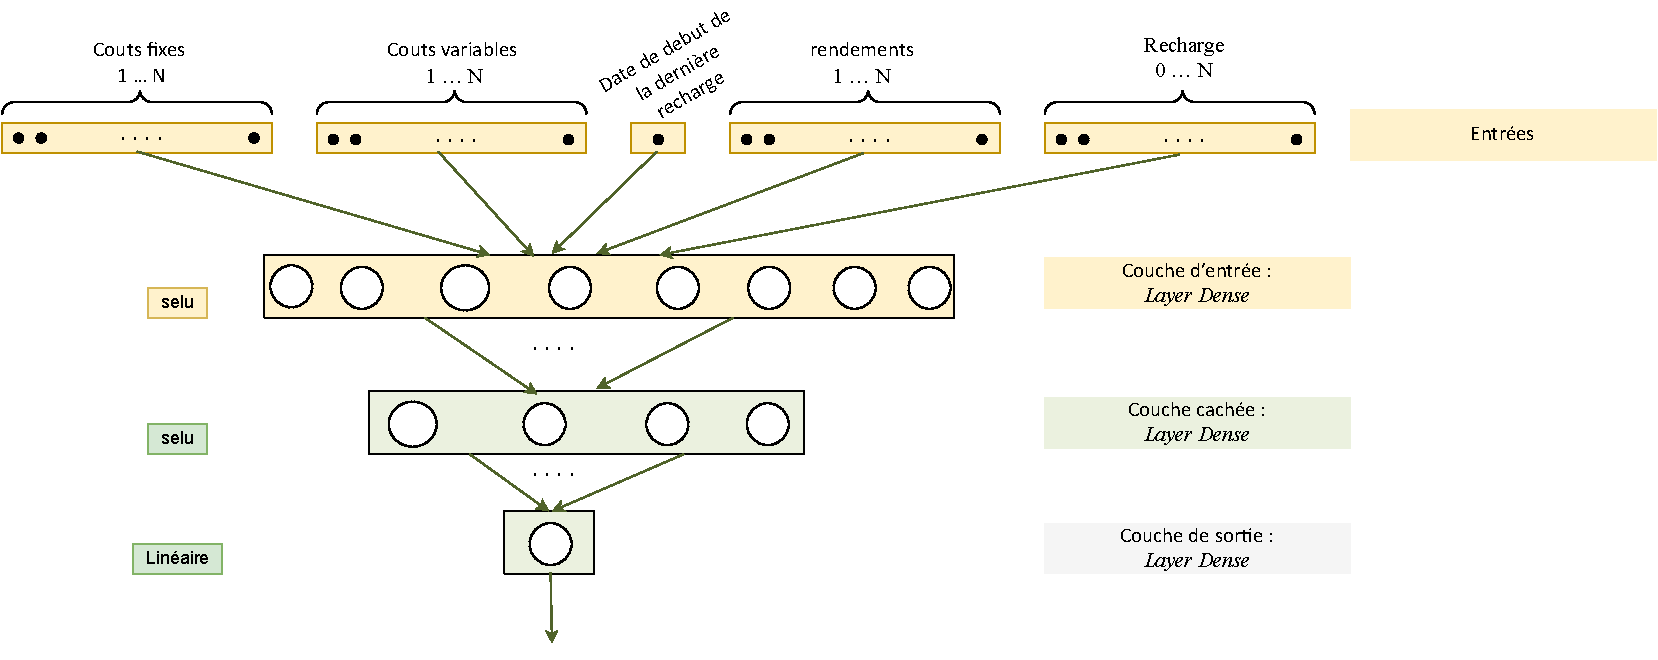
\includegraphics[height=8cm]{images_these/SFC.pdf}}
	\caption[Réseau SIMPLE\_TYPE]{Réseau \textbf{SIMPLE\_TYPE} prédisant le coût de production.}
	\label{SFC}
\end{figure}


\begin{figure}[H]
	\centerline{
		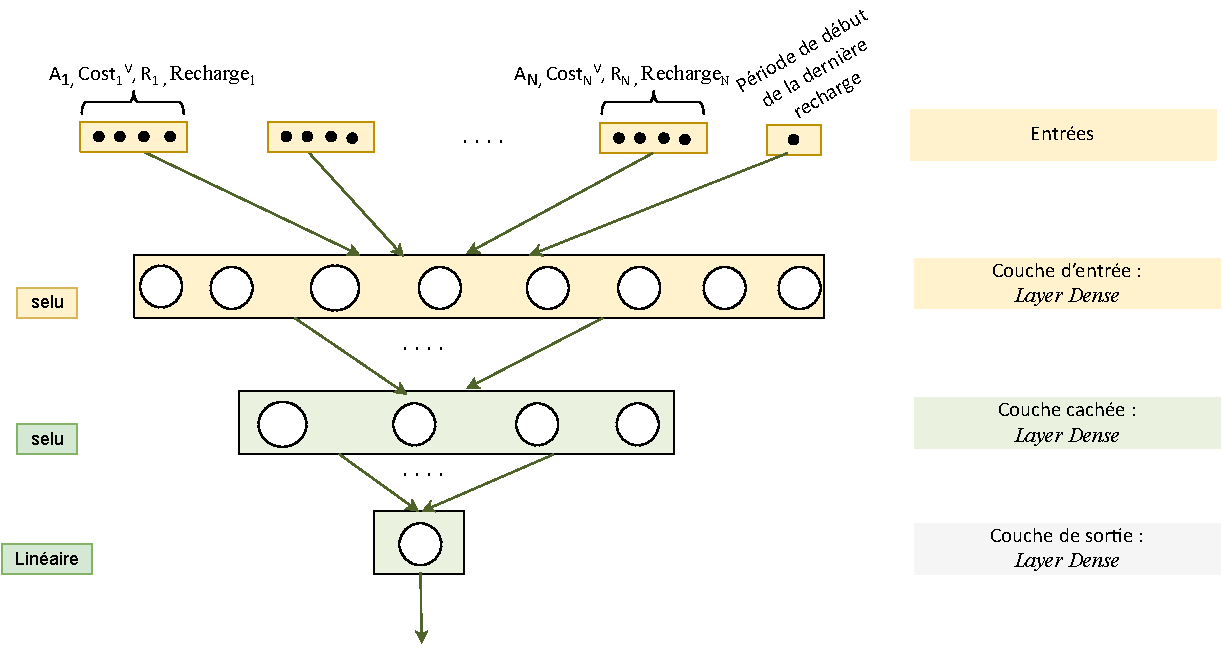
\includegraphics[height=8cm]{images_these/SFC2.pdf}}
	\caption[Réseau SIMPLE\_PERIODE]{Réseau \textbf{SIMPLE\_PERIODE} prédisant le coût de production.}
	\label{SFC2}
\end{figure}

Le nombre de poids et de biais des réseaux de neurones \textbf{SIMPLE\_TYPE} et \textbf{SIMPLE\_PERIODE} dépend de la taille des instances, on a : $8 \times (4N+2)$ poids à la couche d'entrée et 8 biais. Où $N$ est le nombre de périodes. On a $4 \times 8 =32$ poids et 4 biais à la couche cachée. On a 4 poids à la couche de sortie et 1 biais. Dans ce chapitre, puisqu'on travaille uniquement avec des instances de 20 périodes, la couche d'entrées a $8\times(4\times 20 +2)=656$ poids. Si on veut traiter des instances dont le nombre de périodes est hétérogènes, on peut par exemple compresser ces instances.
L'algorithme d'optimisation utilisé est la descente de gradient stochastique. 

%Le taux d'apprentissage $\alpha$ indique la vitesse à laquelle les coefficients évoluent. Plus $\alpha$ sera proche de 1, mieux on corrigera les poids. Autrement dit, les poids varieront avec une assez grande amplitude, puisqu'un exemple pourra augmenter nettement les poids alors qu'un autre pourrait les diminuer nettement.  L'avantage d'un $\alpha$ proche de 1 est que, s'il n'est pas trop proche de 1, il fera converger assez rapidement vers des poids corrects.Le désavantage, c'est que justement s'il est trop proche de 1, on pourrait dans de nombreux cas faire osciller les poids sans jamais converger, ou alors au bout d'un très grand nombre d'itérations. Si $\alpha$ s'éloigne de 1, il corrigera petit à petit les poids sur chaque exemple, sans une grosse variation d'amplitude. L'avantage d'un $\alpha$ éloigné de 1 est que, s'il n'est pas trop éloigné, il fera converger petit à petit mais assez rapidement les poids vers de bonnes valeurs. L'inconvénient c'est que s'il est trop éloigné de 1, les poids varieront tellement doucement qu'on risque de ne jamais les voir converger vers de bonnes valeurs, ou alors encore une fois au bout d'un très grand nombre d'itérations.

%Adam est différent de la descente de gradient stochastique classique. La descente de gradient stochastique maintient un taux d'apprentissage ($\alpha \in [0,1]$) unique pour toutes les mises à jour de poids et le taux d'apprentissage ne change pas pendant l'entraînement. Il est maintenu pour chaque poids de réseau et adapté séparément à mesure que l'apprentissage se déroule. La méthode calcule des taux d'apprentissage adaptatifs individuels pour différents paramètres à partir d'estimations des premiers et second moments des gradients.
 
%Pour finir, la fonction de perte utilisé est le carré des erreurs.
 Les données de validation sont 1/3 des données d'apprentissage. Le nombre d'itérations correspondant à l'itération qui a fournit le plus petit gap sur les données de test est 20 pour le réseau \textbf{SIMPLE\_TYPE} et 3 pour le réseau \textbf{SIMPLE\_PERIODE}. La taille des batchs fixée ici est 32.
\subsubsection{Description des sorties des réseaux de neurones \textbf{SIMPLE\_}}
La sortie des réseaux de neurones \textbf{SIMPLE\_TYPE} et \textbf{SIMPLE\_PERIODE} est le coût de production.
%\subsection{Modèle fonctionnel complètement connecté}

%Voir figure (\ref{reseauFunctional})
%\begin{figure}[H]
%	\centerline{
%		\includegraphics[height=7cm]{images_these/reseauFunctional.pdf}}%je n'ai pas dessiner ceci
%	\caption[Modèle fonctionnel complètement connecté]{Modèle fonctionnel complètement connecté.}
%	\label{reseauFunctional}
%\end{figure}

%Le type d'architecture de réseau de neurones construit dans cette section est limité en terme de topologie de modèle. Il existe un autre type d'architecture qui offre plus de flexiblité dans la conception de la topologie du modèle. Avec cette architecture, on peut construire des réseaux de neurones plus complexes tels que des réseaux \textit{multi-input/multi-output}, des graphiques acycliques orientés (ils ne possèdent pas de circuits), et des réseaux à couches partagées. 
Dans la section suivante, on va construire le réseau \textbf{MIXTE} qui épouse la logique de notre problème.

\subsection{Construction du réseau \textbf{MIXTE} pour la prédiction du coût de production et du numéro de période de la dernière recharge}
%Le réseau \textbf{MIXTE} offre plus de flexibilité pour structurer le réseau de neurones à notre convenance. Avec ce type d'architecture, on peut avoir plusieurs couches d'entrées et plusieurs couches de sorties.
 Notre objectif ici est de construire un réseau de neurones qu'on nomme \textbf{MIXTE} qui épouse les mécanismes de calcul et les caractéristiques du problème de production. Dans cette section, on va décrire les données d'entrée, l'architecture et les données de sortie de notre réseau.
\subsubsection{Description des entrées du réseau de neurones \textbf{MIXTE}}

Les entrées du réseau de neurones \textbf{MIXTE} sont :
\begin{itemize}[label=$\square$]
 \item Le coût d'activation $A=A_i$, avec $i \in \{0, \dots, N-1\}$ puisque dans notre problème le coût d'activation est $Cost^F$, on pose ici $\forall i, A_i=Cost^F$ ;
 \item Pour $i=0, \dots, N-1$, $Cost_i^V$ est le coût de production lié à la période $i$ ;
%\item $C^{Veh}$ capacité du réservoir
\item Pour $i=0, \dots, N-1$, $R_i$ est la rendement de production lié à la période $i$ ;
\item $Q$ est le nombre d'opérations de recharge en carburant effectuées par le véhicule ;
\item $\mu_q$ est la quantité d'hydrogène qui est rechargée lors de la $q^{i\grave eme}$ opération de recharge ;
\item Des bornes inférieures $m_1, \dots,m_Q$ respectivement pour les numéros de période $i_1, \dots, i_Q\in \{0, \dots, N-1\}$ lorsque les opérations de recharge en hydrogène ont lieu ; 
\item 
 On a $N$ périodes $1, \dots, N$ et 2 périodes fictives $0$, $N+1$ ; $Q$ recharges $+ 2$ recharges fictives $(0, Q+1)$ qui modélisent les niveaux de départ et d'arrivée de la citerne ; $\mu_1, \dots, \mu_Q$ : quantité à recharger par le véhicule ; $F_1, \dots, F_Q$  fenêtres de temps pour les recharges ($F_q=[m_q,M_q ]$); $L_1, \dots, L_Q$ longueurs des fenêtres (NB. on suppose connaître exactement les périodes de recharge donc $L_i=1$ $\forall i=1, \dots, N$) ; $\forall q=1, \dots, Q$, $\mu_q^*=\mu_q/L_q$(NB. actuellement on aura $\mu_q^*=\mu_q$)
 
$\forall i \in 1, \dots, N$, $\lambda_i=\sum_{q=1, \dots, Q \lor i\in F_q} \mu_q^*$  ( permet de se ramener à un vecteur indicé sur les périodes)
\item $\lambda_0=-H_0$ et $\lambda_{N+1}=H_0$

\end{itemize}


\begin{Example}
	Calcul du $\lambda$ :
	$N = 6$, $Q = 2$ (5 périodes et 2 recharges)
	
	$F_1=[2,3]$, $F_2=[3,6]$, $\mu_1=8$, $\mu_2=20$, $L_1=2$, $L_2=4$, $H_0=3$
	
	$\mu_1^*=4$, $\mu_2^*=5$
	
	$\lambda_0= -3$, $\lambda_7=3$ (quantités liées aux périodes fictives)
	$\lambda_1=0$, $\lambda_2=\mu_1^*=4$, $\lambda_3=\mu_1^*+\mu_2^*=9$, $\lambda_4=\mu_2^*=5$, $\lambda_5=\mu_2^*=5$, $\lambda_6=\mu_2^*=5$
\end{Example}

%La matrice des entrées étant une matrice creuse car les entrées sont de taille différente, on la remplira de façon cyclique (en répétant les valeurs du début à la fin autant de fois qu'il faut pour atteindre la taille maximal)afin que les données forment une matrice rectangulaire. C'est cette opération qui permettra de connaitre exactement le nombre de valeurs en entrées. \textbf{On considère que la taille de notre réseau est la valeur de $N$ maximale}.

 \subsubsection{Description de l'architecture du réseau de neurones \textbf{MIXTE}}

%expliquer la logique de ce réseau
Notre objectif est de représenter avec un réseau de neurone la formule de calcul du coût de production. On divise nos données en deux catégories à savoir les prix ($Cost_i^V$, $Cost^F$) et les valeurs qui désignent les quantités d'hydrogène ($R_i$, $\lambda_i$). Puis, on normalise chaque catégorie avec la fonction sigmoïde.
On sait que le coût de production est constitué de deux composantes à savoir le coût d'activation de la micro-usine (coût fixe) et le coût de production variable.
On sait que les vecteurs désignant les périodes de production et les périodes de démarrage de la micro-usine sont des vecteurs de booléens. Pour chaque période $i$, on veut connaitre la probabilité $\gamma_i$ qu'elle soit une période de production et la probabilité $\gamma_i^*$ qu'elle soit une période de démarrage de la micro-usine.
Une fois qu'on connaitra les probabilités $\gamma_i$ et $\gamma_i^*$, il suffira de les multiplier (à l'aide d'une couche \textit{Multiply Dense}) respectivement par le coût variable $Cost_i^V$ et par le coût fixe $Cost^F$ puis de sommer les valeurs de toutes les périodes pour obtenir le coût de production car la formule de calcul du coût de production est $COST=\sum_{ i = 0, \dots, N -1} \gamma_i \times Cost_i^V + \gamma_i^* \times Cost^F$.
La probabilité $\gamma_i$ est calculée avec la fonction sigmoïde. La probabilité $\gamma_i^*$ se déduit du vecteur des $\gamma_i$ car si on connait les périodes de production, on peut aisément déduire quelles sont les périodes d'activation de la micro-usine.
Pour le calcul de la probabilité $\tau_i$ que $i$ soit la dernière période de recharge on utilise la fonction softmax car on a qu'une unique dernière période de recharge donc il faut que $\sum_{ i = 0, \dots, N -1}\tau_i=1$. On veut éviter que le calcul du numéro de période de la dernière recharge $T=\sum_{i=1, \dots, N} i \times \tau_i$ soit faussé.
L'architecture du réseau de neurones (Voir figure (\ref{FNFC})) que nous avons conçu est la suivante :

\begin{itemize}[label=$\square$]
	\item Elle a deux couches d'entrées constituées chacune de $N$ neurones ;
	\item Elle a quatre couches cachées constituées chacune de $N$ neurones ;
	\item Elle a deux couches de sortie constituée l'une de $N$ neurones et l'autre d'un neurone.
\end{itemize}   

\begin{figure}[H]
	\centerline{
		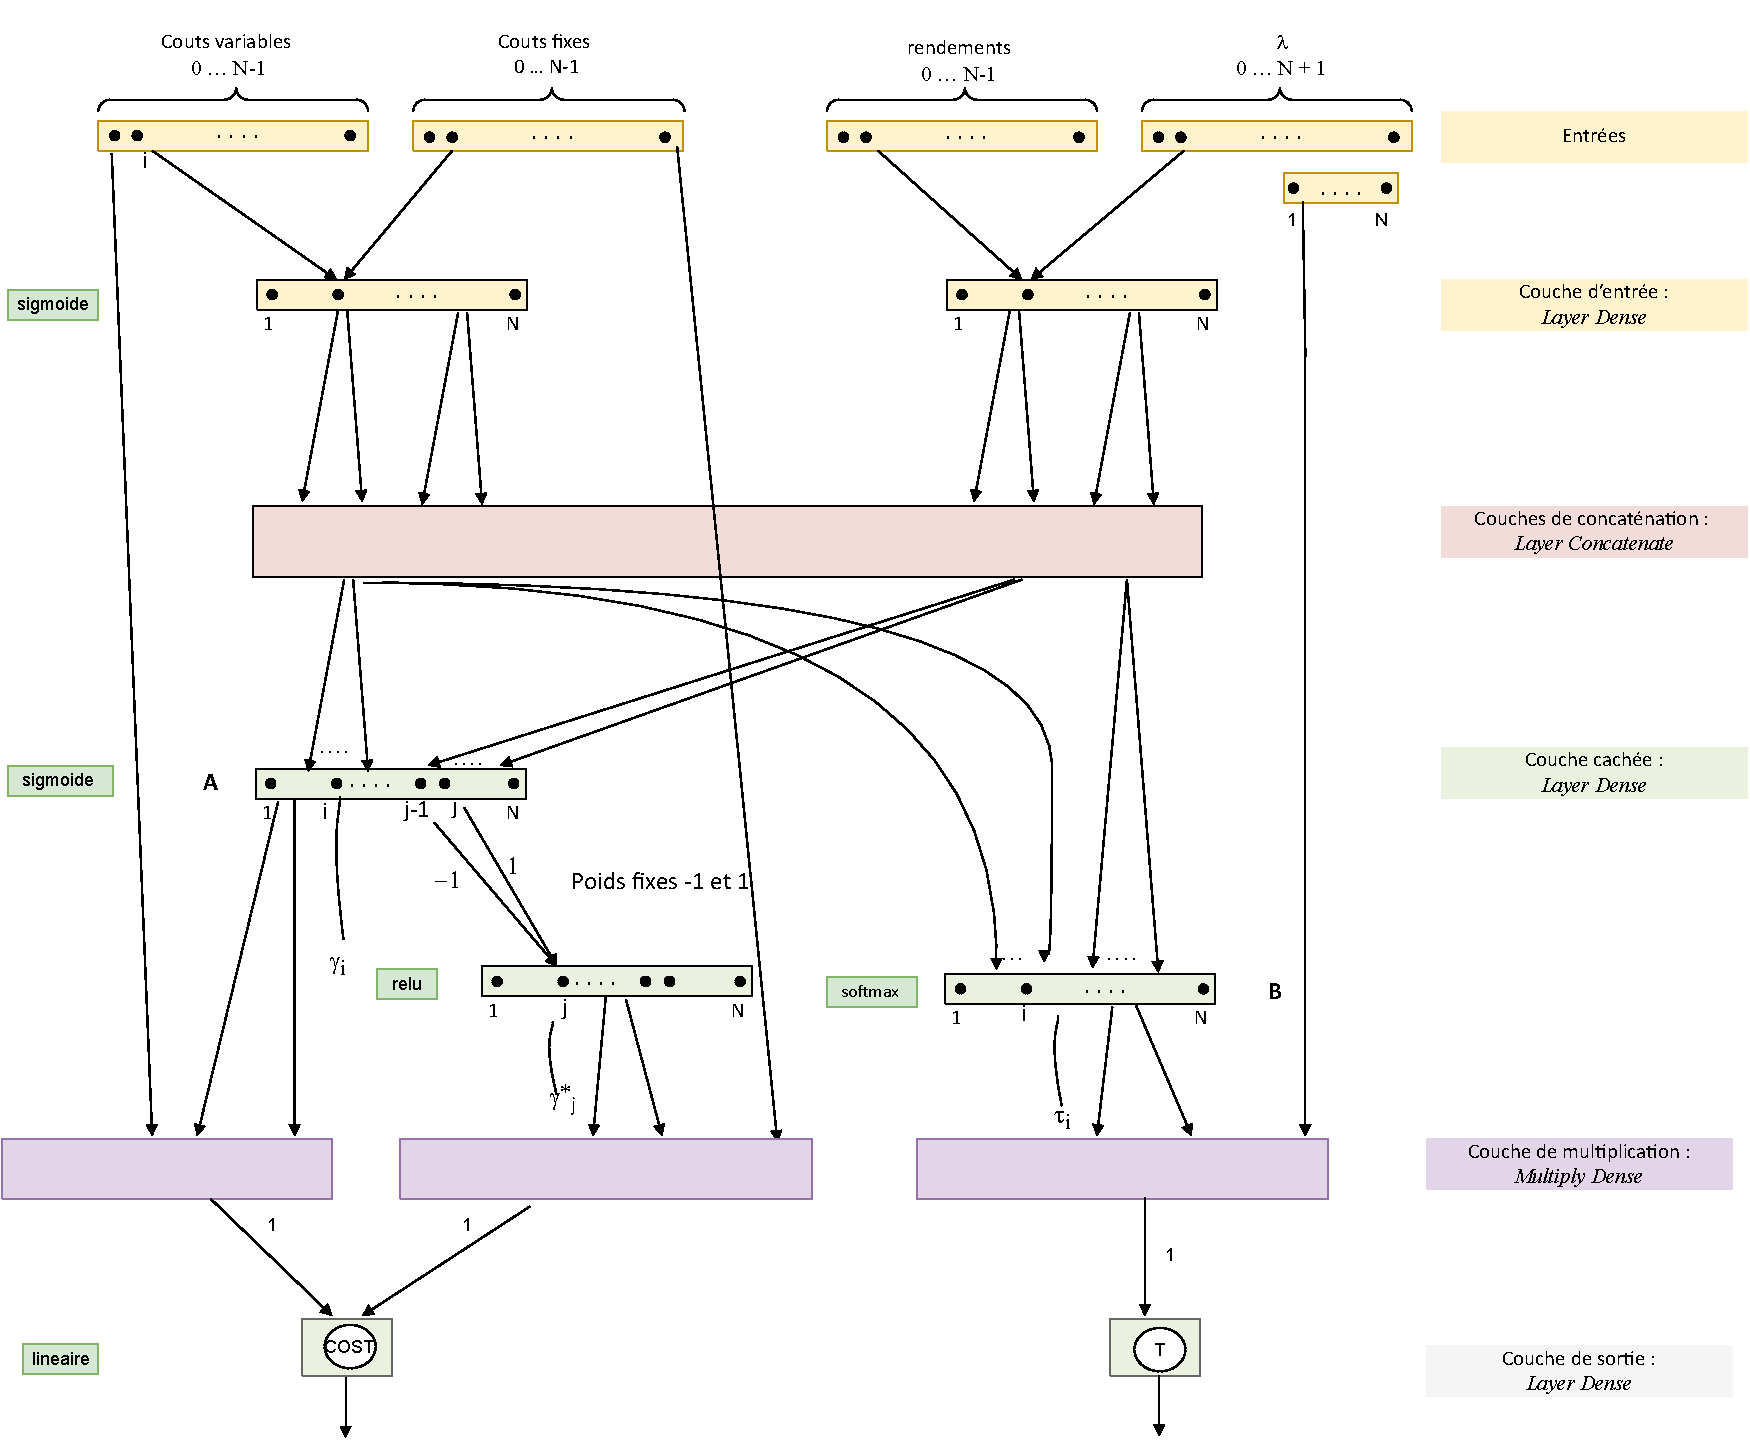
\includegraphics[height=17cm]{images_these/FNFC.pdf}}
	\caption[Réseau MIXTE]{Réseau \textbf{MIXTE} prédisant le coût de production et le numéro de période de la dernière recharge.}
	\label{FNFC}
\end{figure}
Les neurones du réseau ici ne sont pas complètement connectés c'est-à-dire que les neurones d'une couche sont connectés à certains neurones de la couche précédente. Le nombre de neurones des couches a été choisi en fonction du nombre de périodes. Les fonctions d'activation utilisées sont la fonction sigmoïde, la fonction softmax, la fonction RELU ( Elle vaut $x$ si $x$ est supérieur à 0, et 0 sinon. Autrement dit, c'est le maximum entre $x$ et 0) et la fonction linéaire. 

%On a 2*N*N (couche1A) + (2N+2)*N (couche 1B) + 2*N*N (predprod) poids et en plus on a les biais :  (pour les 3 mêmes couches qu'au dessus), ça fait bien 2500 poids en tout avec N = 20.

Le nombre de poids et de biais du réseau de neurones \textbf{MIXTE} est \textbf{quadratique } en fonction de $N$ et de la taille des instances. Le nombre de poids est : $2\times N\times N + (2N+2)\times N + 2\times N \times N=6N^2+2N$. Le nombre de biais est N + N + N. Ce qui fait 2500 poids et biais en tout avec N = 20.
%$2\times N\times N+2\times N\times N+N+N + 2\times N \times N+2\times N\times N=8N^2+2N$.
 L'algorithme d'optimisation utilisé est la descente de gradient stochastique. Les données de validation sont 1/3 des données d'apprentissage. La taille des batchs fixée ici est 32.
 
Pour diminuer le nombre de poids de du réseau \textbf{MIXTE} on décide de supprimer certains poids de la façon suivante : chaque neurone $i$ d'une couche est connecté uniquement aux $i-2$, $i-1$, $i$, $i+1$, $i+2$ de la couche précédente. Lorsqu'on sélectionne les voisins le nombre de neurones devient $2\times N\times N + (2N+2)\times N + 2\times N \times N=188+194+188=570.
 
 
  %La fonction de perte utilisé est lecarré des erreurs. 
%La Fonction d'erreur est :

%$Err=(V-V_{th} )^2$
%avec 
%$V_{th} $ qui représente le coût théorique (prédit) de la solution 
La valeur $V$ est calculée par la formule 
$V=\alpha (\sum_{i=1, \dots, N} i \times \tau_i )+\beta (\sum_{i=1, \dots, N} Cost_i^V \times \gamma_i+\sum_{i=1, \dots, N} A_i \times \gamma_i^*)$.
Ainsi le numéro de période de la dernière recharge est $\sum_{i=1, \dots, N} i \times \tau_i$ et le coût de production est $\sum_{i=1, \dots, N} Cost_i^V \times \gamma_i+\sum_{i=1, \dots, N} A_i \times \gamma_i^*$.
%Donc $V=\alpha$ (durée du tour)+$\beta$ (coût de production)% Vérifier la place de $\alpha$ et $\beta$

Lorsqu'on ne veut traiter que la partie production avec le réseau de neurones de la figure (\ref{FNFC}) on supprime de la couche $B$ à la couche de sortie du réseau. On nomme le réseau ainsi obtenu \textbf{MIXTE\_COUT}. Lorsqu'on ne veut traiter que la partie recharge avec le réseau de neurones de la figure (\ref{FNFC}) on supprime de la couche $A$ à la couche de sortie du réseau. On nomme le réseau ainsi obtenu \textbf{MIXTE\_TEMPS}. Le nombre d'itérations correspondant à l'itération qui a fournit le plus petit gap sur les données de test est 161 pour le réseau \textbf{MIXTE\_COUT} et 195 pour le réseau \textbf{MIXTE\_TEMPS}.


%le réseau de neurones de la figure (\ref{FNFC}) peut être amélioré de cette façon : On met un arc entre un neurone i d'une couche d'entrée et un neurone j de la couche suivante si |i-j| < h Sauf C^{Veh} qui est relié à tous (Voir figure (\ref{FNFC_plus}) ). $h\in N$ est un paramètre pour construire le réseau de neurones (dans un premier temps on prendra $h=\infty$)
%\begin{figure}[H]
%	\centerline{
%		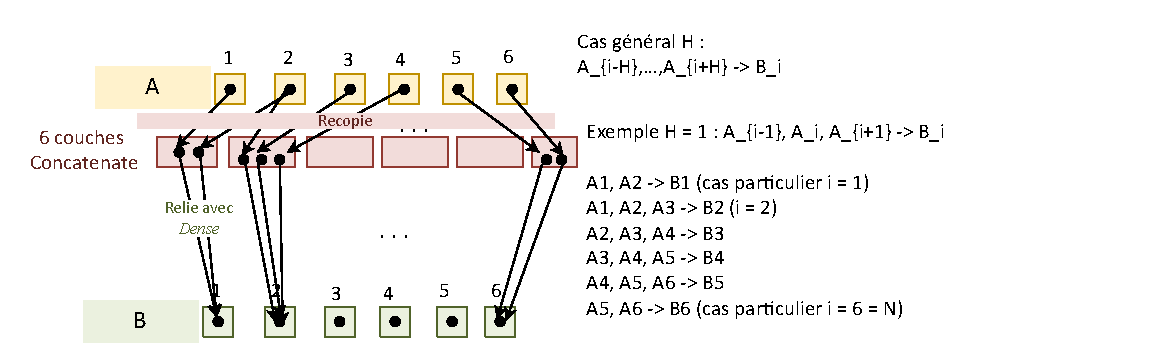
\includegraphics[height=5cm]{images_these/FNFC_plus.pdf}}
%	\caption[Modèle fonctionnel non complètement connecté]{Modèle fonctionnel non complètement connecté.}
%	\label{FNFC_plus}
%\end{figure}
\subsubsection{Description des sorties du réseau de neurones \textbf{MIXTE}}
La sortie de ce réseau de neurones est un vecteur de taille $3N$, leur signification est :
\begin{itemize}[label=$\square$]
	\item $\gamma_i\in [0,1]$, $i=1, \dots, N$ : la probabilité que $i$ soit une période de production
	\item $\gamma_i^*\in [0,1]$, $i=1, \dots, N$ : la probabilité que $i$ soit une période de démarrage de la micro-usine 
	\item $\tau_i^*\in [0,1]$, $i=1, \dots, N$, $\sum_i \tau_i=1$ la probabilité que la période $i$ soit la période de dernière recharge
\end{itemize}
$\gamma_i$ et $\gamma_i^*$ sont agrégés pour calculer le coût de production.

\subsection{Cas des instances aux nombres de périodes hétérogènes}
%Pour cela, on a commencé par présenter des indicateurs et ensuite on a présenté un réseau basé sur les réseaux de neurones pour prédire le coût de production du problème SMEPC.
%Au cas où on veut adapter nos réseaux à des instances dont le nombre de périodes est hétérogènes, on peut transformer les instances dont le nombre d'instances est différent de 20 comme suit :

Les réseaux \textbf{SIMPLE\_TYPE}, \textbf{SIMPLE\_PERIODE}, \textbf{MIXTE\_COUT} et \textbf{MIXTE\_TEMPS} prennent en entrées des données dont la taille doit être fixe, cette taille dépend du nombre de périodes. Or, comme on peut avoir des instances dont le nombre de périodes est différent ( on appelle cela des instances hétérogènes). Pour utiliser ces réseaux sur de telles instances, il va falloir avant tout effectuer un pré-traitement qui consistera à rendre ces instances homogènes, c'est-à-dire faire qu'elle ait le même nombre de périodes. 

Si on décide de considérer que la taille des données d'entrées est la taille de l'instance dont le nombre de période est le plus élevé alors la matrice des entrées sera une matrice creuse car les entrées sont de tailles différentes. On peut la remplir avec des zéros ou alors la remplir de façon cyclique en répétant les données.

Par contre, si on décide de ramener toutes les instances à une taille unique et si par exemple cette taille unique est 20, on peut effectuer la transformation suivante :

\begin{itemize}[label=$\square$]
	\item Si N se situe entre $20.K$ et $20.(K+1)$ avec $K \geq 1$, alors, pour tout $u$ allant de $1$ à $\lceil N/K\rceil$, on fusionne les coefficients des différents vecteurs indexés de $1$ à $N$ de la façon suivante :
	\begin{itemize}
		\item S'il s'agit de $R_i$ qui donne les rendements, on pose $R^*_u = \lceil(\sum_{k.u \leq i < (k+1).u} R_i)/K\rceil$ ;
		\item S'il s'agit de $Cost^V_i$ qui donne les coûts de production, on pose $Cost^V*_u =\lceil (\sum_{k.u \leq i < (k+1).u} Cost^V_i)/K\rceil$ ;
		\item S'il s'agit du coût d'activation $Cost^F$, on pose $Cost^F_u=\lceil Cost^F/K\rceil$  ;
		\item Pour ce qui est des fenêtres de temps $[m_q, M_q]$ et de $\mu_q$, $q = 1, \dots, Q$, sur les périodes et quantités de recharge, on divise chaque quantité $m_q$, $M_q$ et $\mu_q$ par $K$ (division entière).
	\end{itemize}
	\item Quand on obtient le résultat $Cost$ et $T$, où $Cost$ est le coût et $T$ le numéro de période de la dernière recharge, alors on multiplie $Cost$ et $T$ par $K$ pour reconstituer le résultat souhaité.
\end{itemize}

Dans la section suivante, on va construire un autre réseau de neurones dont les entrées sont des indicateurs.
\section{Réseaux de neurones dont les entrées sont des indicateurs}
\label{RN_PM}

Dans les réseaux de neurones précédent, le nombre de poids et de biais du réseau dépend fortement de la taille des instances. Donc si on a des entrées de grande taille on aura un grand nombre de poids et de biais. Pour éviter que la taille de nos réseaux de neurones dépende de la taille des instances on définit dans cette section un ensemble d'indicateurs. Dans cette section, on compacte les entrées de nos réseaux de neurones en un ensemble d'indicateurs de telle sorte que le réseau ait une taille fixe. Autrement dit, on essaye d'agréger les entrées. Au vu de la manière dont les indicateurs évoluent, on suppose qu'on peut les utiliser pour obtenir une approximation du coût de production et du numéro de période de la dernière recharge. Pour cela, on va construire des équations dont les coefficients seront trouvées par des réseaux de neurones.
On présente ici les réseaux de neurones dont les entrées sont des indicateurs. Ces réseaux seront utilisés pour apprendre la valeur du coût de production et du numéro de période de la dernière recharge. Les entrées du modèle SMEPC que nous utiliserons pour construire nos réseaux de neurones pour le problème de production sont présentées au tableau (\ref{inputs_learn}). En plus de ces données, nous aurons aussi besoin des données suivantes :


\begin{itemize}[label=$\square$]
	\item Le coût d'activation $A=A_i$, avec $i \in \{0, \dots, N-1\}$ puisque dans notre problème le coût d'activation est $Cost^F$, on pose ici $\forall i, A_i=Cost^F$;
	\item $Q$ est le nombre d'opérations de recharge en carburant effectuées par le véhicule ;
	\item $\mu_q$ est la quantité d'hydrogène qui est rechargée lors de la $q^{i\grave eme}$ opération de recharge ;
	\item Des bornes inférieures $m_1, \dots,m_Q$ respectivement pour les numéros de période $i_1, \dots,, i_Q\in \{0, \dots, N-1\}$ lorsque les opérations de recharge en hydrogène ont lieu ; 
	
	\item Des bornes supérieures $M_1, \dots,M_Q$ respectivement pour les numéros de période $i_1, \dots,, i_Q \in \{0, \dots, N-1\}$ lorsque les opérations de recharge en hydrogène ont lieu ; 
%	\item Des coefficients de décalage $B_1, \dots, B_{Q-1}$ qui reflètent les contraintes que ces numéros de période doivent satisfaire : pour tout $q = 1, \dots,Q-1$, $i_{q+1} \geq i_q + B_q$.%(nous considérons que $i_0 = 0$ comme une opération de recharge fictive, qui nécessite 0 période). 
	\item Le coût unitaire de production est $P_i=Cost_i^V/R_i$
    \item L'écart du coût unitaire de production est $G_i=|P_{i+1}-P_i|$. $G_i$ est une mesure de désordre des coûts unitaires par rapport au temps. Cette valeur sanctionne le fait que les coûts de production oscillent beaucoup lorsqu'on passe de $i$ à $i+1$.
\end{itemize}
%!!!!!!!!!!!!données dont il faut changer le nom dans ce document:  (Min,m) (Max,M) (A, Cost^F)  (V_i, Cost_i^V)
\subsection{Indicateurs}
%\subsubsection{Liste des indicateurs}
Dans cette section, on définit des indicateurs qui permettent de faire une approximation du coût de production et du temps de parcours du véhicule. On va définir des indicateurs basés sur les moyennes de nos données. On veut calculer des quantités agrégées qui auront un impact prévisible sur le coût de production. Ces quantités agrégées seront utilisées comme entrées de nos réseaux de neurones afin que la taille de ceux-ci ne dépende plus de la taille des instances. On veut donc avoir des réseaux de taille fixe. Les indicateurs encadrés sont ceux qui sont utilisés comme entrées sans aucune modification.
Nous introduisons plusieurs indicateurs comme suit :
\begin{itemize}[label=$\square$]
\item	Indicateurs énergétiques :
\begin{itemize}
\item	\fbox{$Mu = \sum_q \mu_q$} : $Mu$ est la quantité totale d'hydrogène rechargée. Si la valeur de $Mu$ augmente alors la valeur du coût de production a tendance à aussi augmenter;
\item	\fbox{$K = \lceil Mu/ C^{Tank} \rceil$} : $K$ représente le nombre minimum de fois qu'il faudra faire le plein de la citerne de la micro-usine pour pouvoir satisfaire toutes les recharges. $K$ représente aussi le nombre minimum de démarrage de la machine de production. Si la valeur de $K$ augmente alors la valeur du coût de production a tendance à aussi augmenter ;
\item	$R = (\sum_i R_i)/N$ : $R$ est la quantité moyenne de carburant qu'on peut produire par période. Si la valeur de $R$ augmente alors la valeur du coût de production a tendance à diminuer car on aura besoin de moins de périodes pour produire le carburant dont on a besoin ;
\item $R^0 = (\sum_i |R_i- R|)/N$ : $R^0$ est l'écart type des rendements. Cette valeur mesure le désordre dans le temps des rendements de production, plus cette valeur est proche de zéro, plus les $R_i$ sont proches de $R$. %Donc si la valeur de $R$ augmente et que $R^0$ diminue alors la valeur du coût de production a tendance à diminuer car on aura besoin de moins de périodes pour produire le carburant dont on a besoin ;
\end{itemize}
\item	Indicateurs libres :
\begin{itemize}
\item	\fbox{$C = (\sum_i R_i)/Mu$} : $C$ représente la difficulté qu'on a à produire le carburant dont le véhicule aura besoin lors de ses recharges. Plus la valeur $C$ est élevée, plus on aura tendance à pouvoir facilement produire du carburant ;
\item	$C(q) = (\sum_{i \leq M_q} R_i)/(\mu_1 + \dots + \mu_q - H_0)$ : $C(q)$ représente la difficulté qu'on a à produire le carburant dont le véhicule aura besoin à la recharge $q$. Plus les valeurs $C(q)$ sont élevées, plus on aura tendance à pouvoir facilement produire du carburant pour satisfaire les recharges 1 à $q$ ;
\item	\fbox{$C^* = Inf_q C(q)$} : plus la valeur de $C^*$ augmente , plus on aura tendance à pouvoir facilement produire du carburant dont aura besoin le véhicule. Donc plus cette valeur est grande, plus le numéro de période de la dernière recharge aura tendance à diminuer ;
\end{itemize}

\item	Indicateurs de temps : 
\begin{itemize}
\item	$I^0 $ est la plus petite valeur de l'indice $i_0$ tel que $(\sum_{i \leq i_0} R_i) \geq Mu$ ; si on décidait de produire tout le carburant à recharger $Mu$ durant des périodes consécutives en commençant à la première période, $I^0$ est le nombre de périodes qui seraient nécessaire pour produire tout ce que le véhicule va recharger. \fbox{$I^0/N$} $\in ]0,1]$ : plus cette valeur se rapproche de 1, plus on aura tendance à avoir besoin de périodes consécutives pour satisfaire les recharges, ce qui repoussera le numéro de période de la dernière recharge. 
\item	$R^* = (\sum_i i \times R_i)/(\sum_i R_i)$ : $R^*$ est la moyenne des rendements pondérés par les numéros de périodes. Plus cette valeur est grande, plus les meilleurs rendements de production (les plus élevés) auront tendance à se trouver vers la fin de l'espace temps (proche de la période $N$) ;
\item	$P^* = (\sum_i i\times P_i)/(\sum_i P_i)$ : $P^*$ est la moyenne des coûts unitaires pondérés par les numéros de périodes. Plus cette valeur est grande, plus les plus mauvais coûts unitaires de production (les plus élevés) auront tendance à se trouver vers la fin de l'espace temps (proche de la période $N$) ;
\item	$V^* = (\sum_i i \times Cost_i^V)/(\sum_i Cost_i^V)$ : $V^*$ est la moyenne des coûts variables pondérés par les numéros de périodes. Plus cette valeur est grande, plus les plus mauvais coûts variables de production (les plus élevés) auront tendance à se trouver vers la fin de l'espace temps (proche de la période $N$) ;
\item	$A^* = (\sum_i i\times A_i)/(\sum_i A_i)$ :  $A^*$ est la moyenne des coûts fixes pondérés par les numéros de périodes. Plus la valeur \fbox{$A^*/N$} est grande, plus les plus mauvais coûts fixes de production (les plus élevés) auront tendance à se trouver vers la fin de l'espace temps (proche de la période $N$) ;
\item	$G^* = (\sum_i i \times G_i)/(\sum_i G_i)$ :  $G^*$ permet de localiser le désordre dans le temps des coûts unitaires. Si $G^*$ est petit alors le désordre se trouve au début de l'espace temps (car $G_i$ est grand au début de l'espace temps et petit à la fin de l'espace temps). Si on veut tirer parti de ces oscillations, on doit produire au début de l'espace temps. Si le coût d'activation est faible alors la dernière recharge a tendance à être poussé vers la gauche. Si la coût d'activation est faible et que $G^*$ est grand (forte fluctuation des coûts unitaires vers la droite) alors la date de dernière recharge aura tendance à être poussé vers la droite (vers la fin de l'espace temps) car on cherche à produire au coût le plus petit ;
\item	$I(q) =$ le plus petit $i$ tel que $R_1 + \dots + R_i \geq \mu_1 + \dots + \mu_q - H_0$ ; $I(q)$ permet de savoir à partir de quelle période on peut satisfaire la demande $\mu_q$. Autrement dit, la recharge $q$ n'aura pas lieu avant la période $I(q)$. Plus $I(q)$ est grand, plus la date de dernière recharge aura tendance à être poussé vers la droite (vers la fin de l'espace temps) ;
\item	$\Delta(q) = Sup(I(q), m_q) - m_q$ : $\Delta(q)$ est la correction de la fenêtre de temps de la borne inférieur $m_q$ ;
\item	$De = Sup_q \Delta(q)$ : $De$ est la plus grande correction de la fenêtre de temps de la borne inférieur $m_q$. Plus $De$ est grand, plus la date dernière recharge a tendance à être poussé vers la droite (vers la fin de l'espace temps).
\end{itemize} 

\item Indicateurs de coût unitaire :
\begin{itemize}
\item	$P = (\sum_i P_i)/N$ : $P$ est la moyenne des coûts unitaires de production ; plus $P$ augmente, plus le coût de production va avoir tendance à augmenter ; 
\item  $P^0 = (\sum_i |P_i- P|)/N$ : $P^0$ est l'écart type du coût unitaire de production ; $P^0$ mesure le désordre dans les coûts unitaires de production. Si les coûts unitaires sont élevés et qu'il y a une forte variance dans ceux-ci alors on pourra produire facilement à faible coûts. Si $P^0$ augmente alors on peut espérer produire sensiblement moins chère que le prix moyen et si c'est le cas le nombre d'activation aura tendance à augmenter.
%plus cette valeur est proche de zéro, plus les $P_i$ sont proches de $P$. Plus cette valeur diminue et si $P$ augmente, alors ça aura tendance à coûter cher de produire du carburant donc le coût de production va avoir tendance à augmenter ; 
\item	$G = (\sum_i G_i)/N$ : $G$ est la moyenne des écarts des coûts unitaires de production ; Plus $G$ est grand, plus les coûts de production oscillent beaucoup c'est-à-dire qu'on peut trouver des périodes avec de très petits coûts et des périodes avec de très grands coûts.
\item $G^0 = (\sum_i |G_i- G|)/N$ : $G^0$ est l'écart type des écarts des coûts unitaires de production ; $G^0$ mesure le désordre dans le temps des coûts unitaires de production.
\end{itemize}

\item	Indicateurs de coût absolu:
 
\begin{itemize}
\item	$A = (\sum_i A_i)/N$ : $A$ est le coût fixe moyen de production de carburant par période; plus $A$ augmente, plus ça aura tendance à coûter cher de démarrer la micro-usine pour produire du carburant donc le coût de production va avoir tendance à augmenter ;  
\item $A^0 = (\sum_i |A_i- A|)/N$ : $A^0$ est l'écart type des coûts fixes de production ; cette valeur mesure le désordre dans le temps des coûts d'activation. plus cette valeur est proche de zéro, plus les $A_i$ sont proches de $A$. %Plus cette valeur diminue et si $A$ augmente, alors ça aura tendance à coûter cher de démarrer la micro-usine pour produire du carburant donc le coût de production va avoir tendance à augmenter ;
\item	$V = (\sum_i Cost_i^V)/N$ : $V$ est le coût moyen de production variable de carburant par période ;  plus $V$ augmente, plus le coût de production va avoir tendance à augmenter ;
\item $V^0 = (\sum_i |Cost_i^V- V|)/N$ :  $V^0$ est l'écart type des coûts de production variables ; cette valeur mesure le désordre dans le temps des coûts de production variable. plus cette valeur est proche de zéro, plus les $V_i$ sont proches de $V$. Plus $V^0$ est grand plus on peut espérer trouver de bonnes valeurs c'est-à-dire qu'on peut espérer produire sensiblement moins chère que le coût de production variable moyen.%Plus cette valeur diminue et si $V$ augmente, alors ça aura tendance à coûter cher de produire du carburant donc le coût de production va avoir tendance à augmenter.
\end{itemize}
\end{itemize}
Ici, on a raisonné avec la possibilité qu'on a des coûts d'activation variable, mais dans notre problème on a un cout d'activation fixe donc $A$ est le coût d'activation et $A^0$ vaut 0.


\begin{Example}
	Reprenons l'exemple (\ref{exemple_synchronisation}) avec les entrées $H_0=4$, $C^{Tank}=15$, les valeurs des indicateurs sont $Mu = 25$, $K = 2$, $R=2,666$, $R^0=1,2$, $C=1,6$, $C(1)=1,8$, $C(2)=1$, $C^*=1$, $I^0 = 8$, $R^* =7,075$, $P^* =9,396$, $V^* =8,385$, $A^* =8$, $G^* =4,467$, $I(1) =1$, $I(2) =7$, $\Delta(1)=0$, $\Delta(2)=0$, $De=0$, $P=0,851$, $P^0=0,472$, $G=0,033$, $G^0=0,387$, $A=3$, $A^0=0$, $V=1,733$, $V^0=0,684$.
\end{Example}

\begin{Example}
	Reprenons l'exemple (\ref{ex_rech_2}) avec les entrées $H_0=1$, $C^{Tank}=105$,  les valeurs des indicateurs sont $Mu =96$, $K =1 $, $R=15,367$, $R^0=6,682$, $C=4,802$, $C(1)=4,72$, $C(2)=6,545$, $C(3)=3,955$, $C(4)=3,926$, $C^*=3,926$, $I^0 =6 $, $R^* =14,575$, $P^* =13,169$, $V^* =10,719$, $A^* =15,5$, $G^* =-0,319$, $I(1) =2$, $I(2) =2$, $I(3) =4$, $I(4) =6$, $\Delta(1)=0$, $\Delta(2)=0$, $\Delta(3)=0$, $\Delta(4)=0$, $De=1$, $P=0,156$, $P^0=0,104$, $G=-0,032$, $G^0=0,133$, $A=13$, $A^0=0$, $V=2,133$, $V^0=1,457$.
\end{Example}

\subsection{Construction du réseau \textbf{INDIC\_TEMPS} pour la prédiction du numéro de période de la dernière recharge}
Dans cette section, on va décrire les données d'entrée, l'architecture et les données de sortie de notre réseau pour la prédiction de la date de la dernière recharge.
\subsubsection{Description des entrées du réseau de neurones \textbf{INDIC\_TEMPS}}
Dans cette section, on identifie les valeurs qui ont une influence pour la prédiction du numéro de période de la dernière recharge. Ces valeurs seront les entrées du réseau de neurones. Les entrées du réseau de neurones \textbf{INDIC\_TEMPS} sont :
\begin{itemize}[label=$\square$]
\item $H_0/Mu$ : plus la valeur $H_0/Mu$ est grande, plus la date de la dernière recharge aura tendance à diminuer car on aura tendance à ne pas produire car la quantité d'hydrogène initiale de la citerne est suffisante pour assurer les recharges du véhicule ;
\item $P^*/N$ : plus la valeur $P^*/N$  est grande, plus la date de la dernière recharge aura tendance à diminuer car on aura tendance à vouloir produire plus tôt car les meilleurs coûts de production variable s'y trouvent ;
\item $A^*/N$ : plus la valeur $A^*/N$ est grande, plus la date de la dernière recharge aura tendance à diminuer car on aura tendance à vouloir produire plus tôt car les meilleurs coûts d'activation s'y trouvent ;
\item $C$ : plus la valeur $C$ est grande, plus la date de la dernière recharge aura tendance à diminuer ;
\item $C^*$ : plus la valeur $C^*$ est grande, plus la date de la dernière recharge aura tendance à diminuer ;
\item $K$ : si la valeur de $K$ augmente alors la valeur de la date de la dernière recharge aura tendance à augmenter ;
\item $I^0/N$ $\in ]0,1]$ : plus la valeur $I^0/N$ se rapproche de 1, plus le nombre de périodes consécutives dont on aura besoin pour satisfaire les recharges aura tendance à augmenter, ce qui aura tendance à augmenter la date de la dernière recharge ; 
\item $[m_Q, M_Q]$ : c'est l'intervalle de temps durant laquelle la dernière recharge doit être réalisée.
%\item 1
\end{itemize}
\poubelle{
Pour chaque entrée ci-dessus on a récupérer le minimum, le maximum, la moyenne et l'écart type de nos instances :
\begin{itemize}[label=$\square$]
\item $H0/Mu$ : min= 0, max= 0.9924242424242424, moy= 0.28822644413495735, ecartType= 0.19111705864482398
\item $P^*/N$ : min= 0.07009907150626704, max= 0.8613313564935897, moy= 0.5260700128578728, ecartType= 0.19111705864482398
\item $A^*/N$ : min= 0.525, max= 0.525, moy= 0.525, ecartType= 0.19111705864482398
\item $C$ : min= 1.0384615384615385, max= 7.847368421052631, moy= 2.2868343061611682, ecartType= 0.19111705864482398
\item $C^*$ : min= 1.0, max= 384.0, moy= 3.478490624380088, ecartType= 0.19111705864482398
\item $K$ : min= 1, max= 3, moy= 1.4257376229371561, ecartType= 0.19111705864482398
\item $I^0/N$ : min= 0.1, max= 1.0, moy= 0.5281796966161028, ecartType= 0.19111705864482398
\item Coût d'activation : min= 5, max= 1500, moy= 257.50541756959495, ecartType= 212.78638412705467
\item Coût de Production sans le coût d'activation : min : 4, max= 1269, moy= 314.76329388231375, ecartType= 247.4793755442504
\item Nombre d'activation : min= 1.0, max= 10.0, moy= 3.4480746791131853, ecartType= 1.63065601837
\end{itemize}
}
\subsubsection{Description de l'architecture du réseau de neurones \textbf{INDIC\_TEMPS}}


Notre but est de calculer des indicateurs qu'on manipulera à travers des équations pour faire une approximation du numéro de période $T$ de la dernière opération de recharge en carburant. 
%Nous voulons obtenir une approximation du numéro de période $T$ de la dernière opération de recharge en carburant. 
Le calcul de $T$ dépend de l'intervalle $[m_Q,M_Q]$. On cherche un barycentre qui correspond au numéro de période de la dernière recharge compris entre $m_Q$ et $M_Q$. Si $Ga$ se rapproche de 1 alors la date de la dernière recharge a tendance à se rapprocher de $m_Q$, il faut ajouter à $m_Q$ la plus grande correction $De$ pour que le véhicule ait le temps de réaliser toutes les recharges. Si $Ga$ se rapproche de 0 alors la date de la dernière recharge a tendance à se rapprocher de $M_Q$. On va écrire ces équations en respectant le sens des indicateurs, ces derniers seront positifs ou négatifs en fonction de l'impact qu'ils ont sur $T$ sachant que notre objectif global est que $T$ soit le plus petit possible c'est-à-dire qu'il se rapproche de $m_Q$. Les indicateurs utilisés pour calculer $X$ sont positifs lorsqu'ils poussent $X$ vers la droite ($X$ devient de plus en plus grand). Les indicateurs utilisés pour calculer $X$ sont négatifs lorsqu'ils poussent $X$ vers la gauche ($X$ devient de plus en plus petit). Plus les valeurs positives de $X$ augmentent plus la date de dernière recharge diminue (se rapproche de $m_Q$). Et, plus les valeurs négatives de $X$ augmentent plus la date de dernière recharge augmente (se rapproche de $M_Q$). Les coefficients des équations seront trouvés à l'aide d'un réseau de neurones. Donc nous définissons :

\begin{itemize}[label=$\square$]
\item	$T = Ga \times (m_Q + De) + (1 - Ga) \times M_Q$ avec $Ga \in  [0, 1]$ ;
\item	$Ga = \Phi^x(X)$, où $\Phi^x$ est une fonction sigmoïde $Exp(x.X)/(Exp(x.X)+1)$, $x \geq 0$;
\item $X = w_0.(H_0/Mu)+w_1.(P^*/N) +  w_2.(A^*/N) +  w_3.C +  w_4.C^* - w_5.K - w_6.I^0/N - w_7$,  où $w_0, w_1, \dots, w_6 \geq 0$ et $w_7$ est non signé.
\end{itemize}
A partir de ces équations, nous construisons l'architecture du réseau de neurones (Voir figure (\ref{time_value_scheme})). L'architecture est la suivante : 

\begin{itemize}[label=$\square$]
	\item Elle a huit couches d'entrées constituées chacune d'un neurone ;
	\item Elle a six couches cachées ;
	\item Elle a une couche de sortie d'un neurone.
\end{itemize}  


\begin{figure}[H]
	\centerline{
		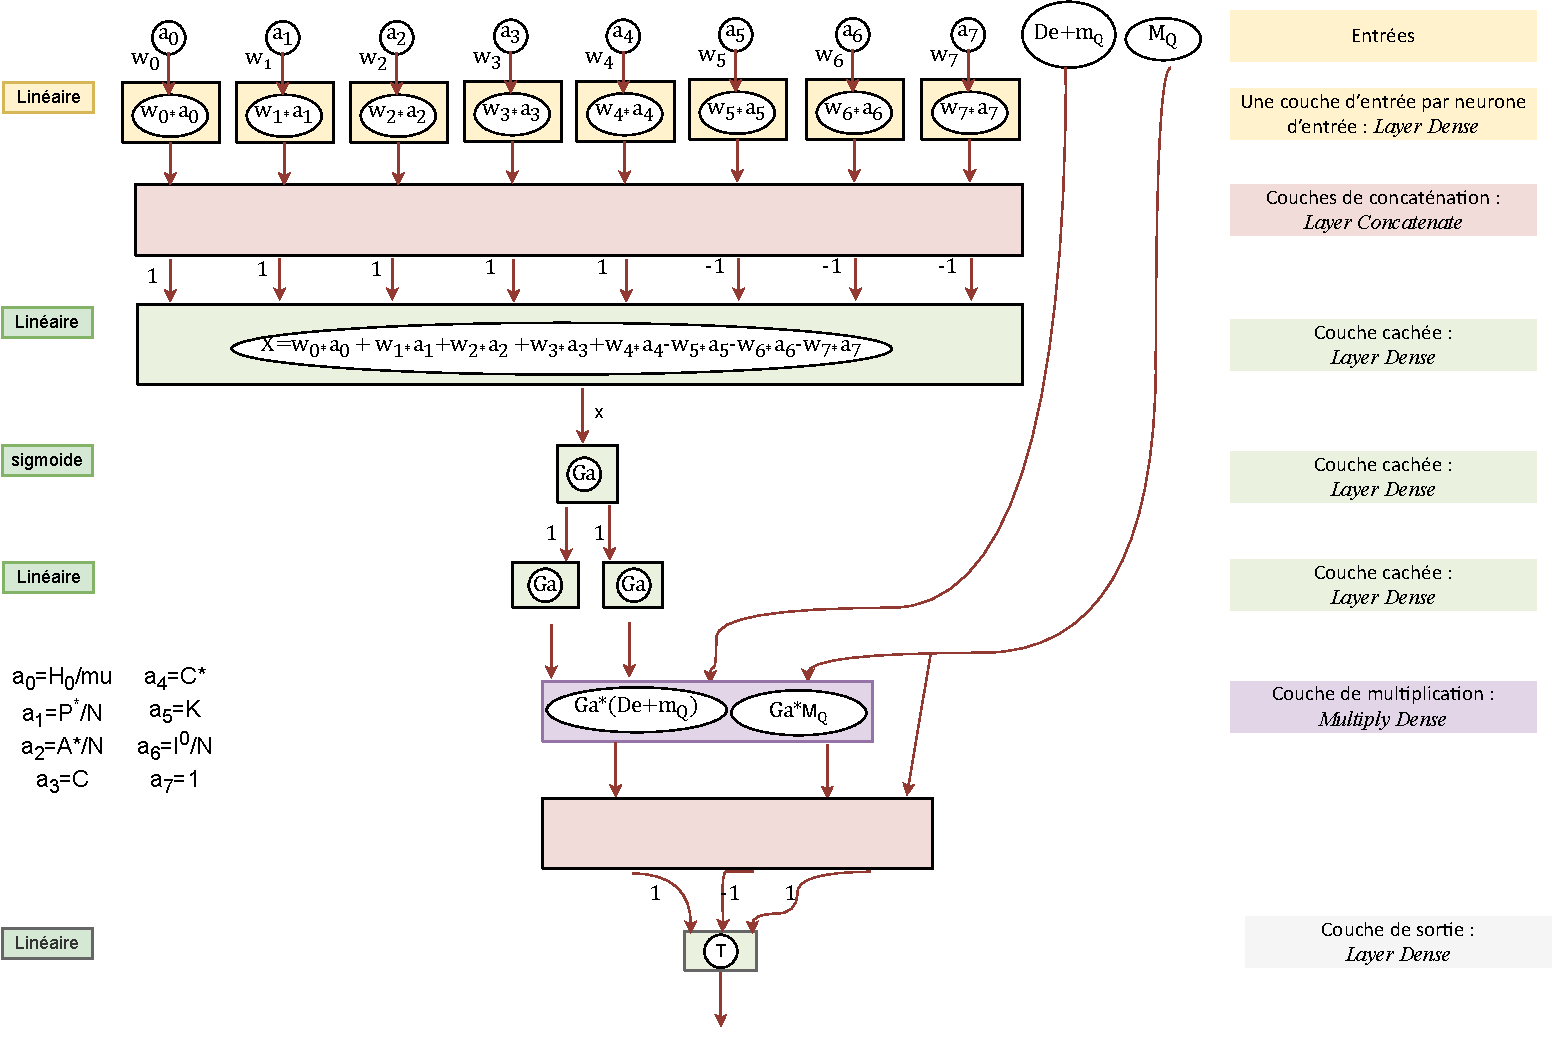
\includegraphics[height=12cm]{images_these/time_value_scheme.pdf}}
	\caption[Réseau INDIC\_TEMPS prédisant le numéro de période de la dernière recharge]{Réseau  INDIC\_TEMPS prédisant le numéro de période de la dernière opération de recharge. Les $w_i$ sont les coefficients synaptiques ou poids.}
	\label{time_value_scheme}
\end{figure}


 Les fonctions d'activation utilisées sont la fonction sigmoïde et la fonction linéaire.
Le nombre de poids et de biais du réseau de neurones \textbf{INDIC\_TEMPS} ne dépend pas de la taille des instances. L'algorithme d'optimisation utilisé est la descente de gradient stochastique. Les données de validation sont 1/3 des données d'apprentissage. Le nombre d'itérations correspondant à l'itération qui a fournit le plus petit gap sur les données de test est 3. La taille des batchs fixée ici est 32.  %La fonction de perte utilisé est lecarré des erreurs. 

Dans le réseau \textbf{INDIC\_TEMPS}, on a 9 poids à apprendre. 
\poubelle{
Les valeurs des poids après apprentissage sont : 
\begin{itemize}[label=$\square$]
\item $x=0.08248362$ ;
\item $w_0=0.60550255$ ;
\item $w_1=0.46121672$ ;
\item $w_2=0.67664534$ ;
\item $w_3=0.8657591$ ; 
\item $w_4=1.1487997$ ;
\item $w_5=1.8023789$ ; 
\item $w_6=0.2762828$ ;
\item $w_7=-1.0792339$.
\end{itemize}
}
%
%Le minimum, le maximum, la moyenne et l'écart type des entrées sont :
%\begin{itemize}[label=$\square$]
%\item H0/Mu : min= 0.0, max= 0.9924242424242424, moy= 0.28822644413495735, ecartType= 0.19111705864482398
%\item P*/N : min= 0.07009907150626704, max= 0.8613313564935897, moy= 0.5260700128578728, ecartType= 0.19111705864482398
%\item A*/N : min= 0.525, max= 0.525, moy= 0.525, ecartType= 0.19111705864482398
%\item C : min= 1.0384615384615385, max= 7.847368421052631, moy= 2.2868343061611682, ecartType= 0.19111705864482398
%\item C* : min= 1.0, max= 384.0, moy= 3.478490624380088, ecartType= 0.19111705864482398
%\item K : min= 1, max= 3, moy= 1.4257376229371561, ecartType= 0.19111705864482398
%\item I0/N : min= 0.1, max= 1.0, moy= 0.5281796966161028, ecartType= 0.19111705864482398
%\end{itemize}
%
%\begin{itemize}[label=$\square$]
%\item Coût d'activation : min= 5, max= 1500, moy= 257.50541756959495, ecartType= 212.78638412705467
%\item Coût de Production sans activation : min= 4, max= 1269, moy= 314.76329388231375, ecartType= 247.4793755442504
%\item Nombre d'activation : min= 1.0, max= 10.0, moy= 3.4480746791131853, ecartType= 1.6306560183759389
%\end{itemize}


\subsubsection{Description des sorties du réseau de neurones \textbf{INDIC\_TEMPS}}
La sortie du réseau de neurones \textbf{INDIC\_TEMPS} est $T$ le numéro de période de la dernière recharge.
\subsection{Construction du réseau \textbf{INDIC\_COUT} pour la prédiction du coût de production}
Dans cette section, on va décrire les données d'entrée, l'architecture et les données de sortie de notre réseau pour la prédiction du coût de production.
\subsubsection{Description des entrées du réseau de neurones \textbf{INDIC\_COUT}}
Dans cette section, on identifie les valeurs qui ont une influence pour la prédiction du coût de production. Ces valeurs seront les entrées du réseau de neurones.
Les entrées du réseau de neurones \textbf{INDIC\_COUT} sont :
%\begin{itemize}[label=$\square$]
%	\item $PR/A$ : on multiplie la moyenne des coûts unitaires par le rendement moyen de production. Si cette valeur augmente alors le nombre d'activation aura tendance à aussi augmenter ;
%	\item $RP^0/A$ : on multiplie l'écart type des coûts unitaires par le rendement moyen de production. Si cette valeur augmente alors le nombre d'activation aura tendance à aussi augmenter ; 
%	\item $RG/A$ : on multiplie la moyenne des écarts des coûts unitaires par le rendement moyen de production. Si $R$ est grand alors cela veut dire qu'on peut facilement produire du carburant. Si $G$ est grand alors on peut choisir les périodes dont le coût est bas. Si $A$ est petit alors on peut faire plusieurs setup sans que cela n'ait une grande influence sur le coût final. Dans ce cas, Si $RG/A$ augmente alors le nombre d'activation aura tendance à aussi augmenter ;
%	\item $A/PR$ : Si $A/PR$ augmente alors le nombre d'activation aura tendance à aussi diminuer ;
%	\item $A^*/N$ : Plus $A^*/N$ est grande, plus les plus mauvais coûts fixes de production (les plus élevés) se trouvent vers la fin de l'espace temps (proche de la période $N$) ; Si cette valeur augmente alors le coût de production aura tendance à aussi augmenter ; %!!aucune incidence sur le coût
%	\item Si les valeurs $A-A^0$ et $A+A^0$ augmentent alors le coût d'activation de la micro-usine aura tendance à aussi augmenter, mais pour notre problème ces valeurs sont statiques.
%	\item $P^*/N$ : Si $P^*/N$ augmente  cela veut dire que les coûts de production sont bons au début alors on aura tendance à produire plus tôt. Donc la date de dernière recharge aura tendance à diminuer et le coût à être plus petit ; 
%	\item $G/P$ : c'est un coefficient de désordre ; c'est la moyenne des écarts des coûts unitaires divisé par la moyenne des coûts unitaires ; si le coût d'activation est petit alors on peut choisir les bonnes périodes.
%	\item $V^0/V$ : c'est le désordre dans les coûts de production. c'est l'écart type des coûts de production variable divisé par le coût de production variable moyen ; si $V^0/V$ augmente cela veut dire qu'il y a du désordre alors on peut produire aux meilleures périodes si le coût d'activation est faible.
%	\item $C$ : si $C$ augmente alors le coût de production aura tendance à aussi diminuer ; 
%	%\item $1$
%	\item Si les valeurs $P-P^0$ et $P+P^0$ augmentent alors le coût de production variable aura tendance à aussi augmenter ;
%	\item $K$ : c'est le nombre minimum de fois qu'il faut faire de le plein de la citerne pour satisfaire toutes les recharges.si cette valeur augmente alors le coût de production aura tendance à aussi augmenter ; 
%	
%	\item $Mu$ : c'est la quantité totale d'hydrogène à recharger.si cette valeur augmente alors le coût de production aura tendance à aussi augmenter.
%\end{itemize}
\begin{itemize}[label=$\square$]
	\item $P/A $ : Si cette valeur augmente alors le nombre d'activation aura tendance à aussi augmenter ;
	\item $P^0/A $ : Si cette valeur augmente alors le nombre d'activation aura tendance à aussi augmenter ;
	\item $G/A$ : Si cette valeur augmente alors le nombre d'activation aura tendance à aussi augmenter ;
	\item $C/A$ : Si cette valeur augmente alors le nombre d'activation aura tendance à aussi diminuer ;
	\item $P^*/N $ : Si $P^*/N$ augmente  cela veut dire que les coûts de production sont bons au début alors on aura tendance à produire plus tôt. Donc la date de dernière recharge aura tendance à diminuer et le coût à être plus petit ; 
	\item $P^0/P$ : c'est le désordre dans les prix unitaires de production. si $P^0/P$ augmente cela veut dire qu'il y a du désordre alors on peut produire aux meilleures périodes si le coût d'activation est faible ;
	\item $A/PR$ : Si $A/PR$ augmente alors le nombre d'activation aura tendance à aussi diminuer ;
	\item $V0/V$ : : c'est le désordre dans les coûts de production. c'est l'écart type des coûts de production variable divisé par le coût de production variable moyen ; si $V^0/V$ augmente cela veut dire qu'il y a du désordre alors on peut produire aux meilleures périodes si le coût d'activation est faible ;
	
	\item $C$ : si $C$ augmente alors le coût de production aura tendance à aussi diminuer ; 
	\item $S/N$ : $S$ est le nombre de recharge. Si cette valeur augmente alors le nombre d'activation aura tendance à aussi diminuer ;
	\item Si les valeurs $P-P^0$ et $P+P^0$ augmentent alors le coût de production variable aura tendance à aussi augmenter ;
	\item $K$ : c'est le nombre minimum de fois qu'il faut faire de le plein de la citerne pour satisfaire toutes les recharges.si cette valeur augmente alors le coût de production aura tendance à aussi augmenter ; 
	
	\item $Mu$ : c'est la quantité totale d'hydrogène à recharger.si cette valeur augmente alors le coût de production aura tendance à aussi augmenter.
\end{itemize}
\poubelle{
Pour chaque entrée ci-dessus on a récupérer le minimum, le maximum, la moyenne et l'écart type de nos instances :


\begin{itemize}[label=$\square$]
	\item $P/A$ :min= 0.005120702150911672, max= 0.5466666666666666, moy= 0.07827778207999901, ecartType= 0.06066775190153355
	\item $P^0/A$ : min= 0.002159267236754706, max= 0.7921712103139121, moy= 0.06660871783569629, ecartType= 0.05896242377607617
	\item $G/A$ : min= 0.0026223198008490543, max= 0.6039761904761904, moy= 0.08232651799236021, ecartType= 0.06940453551561392
	\item $C/A$ : min= 0.007185185185185185, max= 1.4382978723404256, moy= 0.11252805943551572, ecartType= 0.19472746663198043
	\item $P^*/N$ : min= 0.07009907150626704, max= 0.8613313564935897, moy= 0.5260700128578728, ecartType= 0.09479526655910912
	\item $P^0/P$ : min= 0.26992057190123936, max= 1.8234383902705669, moy= 0.8170531854147316, ecartType= 0.21568106994551117
	\item $A/PR$ : min= 0.04141533052086945, max= 3.1536741394609553, moy= 1.0156003266794074, ecartType= 0.5653711362587436
	\item $V^0/V$ : min= 0.07938931297709924, max= 1.0789473684210527, moy= 0.2584961513076968, ecartType= 0.1451619941778243
	\item $C$ : min= 2.2826923076923076, max= 2.2826923076923076, moy= 2.2826923076923076, ecartType= 0.0
	\item $S/N$ : min= 0.05, max= 0.5, moy= 0.17240373395565928, ecartType= 0.08153280091879694
	\item $P-P^0$ : min= -5.655197007460952, max= 14.142666666666663, moy= 0.917376986032352, ecartType= 1.6124441343008649
	\item $P+P^0$ : min= 0.15096527692911665, max= 56.38599206349207, moy= 9.291208290710047, ecartType= 8.829175975588251
	\item $K$ : min= 1, max= 3, moy= 1.4257376229371561, ecartType= 0.5100533085531468
	\item $Mu$ : min= 40,max= 672, moy= 211.9953325554259, ecartType= 117.28149244288375
	\item $A$ : min= 5.0, max= 150.0, moy= 80.98849808301384, ecartType= 49.4329205759421
	
\end{itemize}
}
\subsubsection{Description de l'architecture du réseau de neurones \textbf{INDIC\_COUT}}
Notre but est de produire le plus tôt possible au meilleur coût donc on aimerait que les meilleurs coûts soit plutôt au début de l'espace temps pour pouvoir finir la tournée le plus tôt possible.
On veut calculer des indicateurs qu'on manipulera à travers des équations pour faire une approximation du coût de production $COST$.
 On va écrire ces équations en respectant le sens des indicateurs, ils seront positifs ou négatifs en fonction de l'impact qu'ils ont sur $COST$. Les coefficients des équations seront trouvés à l'aide d'un réseau de neurones.
 
 Dans un premier temps, on veut faire une approximation du coût $Cost_A$  de chaque activation de la micro-usine, le coût total d'activation est environ $Cost_A\times K$, où $K$ est le nombre minimum de fois qu'il faut faire le plein de la citerne pour satisfaire toutes les recharges. $Ta$ doit exprimer la pression qu'on a sur le nombre d'activation minimal. On sait qu'au cours du procédé on aura au moins une activation. d'où $1+Ta$. La valeur $1+Ta$ est un coefficient multiplicateur qu'on appliquera au coût d'activation. 
 %La formule de $Cost_A=(1 + Ta).(Be(A - A^0) + (1 - Be).(A + A^0))$ tient compte du cas où les coûts d'activation sont variables.
  Étant donné que  dans notre problème $A$ vaut le coût d'activation et que $A^0=0$, la valeur $Cost_A = (1 + Ta)\times A$.
  
  Dans un second temps, on veut faire une approximation du coût $Cost_P$ par unité de production, le coût de production sera environ $Cost_P\times Mu$, où $Mu$ est la quantité totale d'hydrogène à recharger.
  Le calcul de $Cost_P$ dépend de l'intervalle $[0,2P]$. Si $\alpha_1$ et $\alpha_2$ se rapprochent de 1 alors le coût $Cost_P$ a tendance à se rapprocher de $2P$. Si $\alpha_1$ et $\alpha_2$ se rapprochent de $0$ alors le coût $Cost_P$ a tendance à se rapprocher de 0. On va écrire nos équations en respectant le sens des indicateurs, ces derniers seront positifs ou négatifs en fonction de l'impact qu'ils ont sur $Cost_P$ sachant que notre objectif global est qu'il soit le plus petit possible c'est-à-dire qu'il se rapproche de $0$. Les indicateurs utilisés pour calculer $Z_1$ et $Z_2$ sont positifs lorsqu'ils poussent $Z_1$ et $Z_2$ vers la droite (ils deviennent de plus en plus grand). Les indicateurs utilisés pour calculer $Z_1$ et $Z_2$ sont négatifs lorsqu'ils poussent $Z_1$ et $Z_2$ vers la gauche (ils deviennent de plus en plus petit). Plus les valeurs positives de $Z_1$ et $Z_2$ augmentent plus $Cost_P$ se rapproche de 0. Et, plus les valeurs négatives de $Z_1$ et $Z_2$ augmentent plus $Cost_P$ se rapproche de $2P$.
 
 %Dans un second temps, on veut faire une approximation du coût $Cost_P$ par unité de production, le coût de production sera environ $Cost_P\times Mu$, où $Mu$ est la quantité totale d'hydrogène à recharger.
 %Le calcul de $Cost_P$ dépend de l'intervalle $[P - P^0,P + P^0]$. On cherche un barycentre qui correspond au coût $Cost_P$ compris entre $P - P^0$ et $P + P^0$. Si $Al$ se rapproche de 1 alors le coût $Cost_P$ a tendance à se rapprocher de $P - P^0$. Si $Al$ se rapproche de 0 alors le coût $Cost_P$ a tendance à se rapprocher de $P + P^0$. On va écrire nos équations en respectant le sens des indicateurs, ces derniers seront positifs ou négatifs en fonction de l'impact qu'ils ont sur $Cost_P$ sachant que notre objectif global est qu'il soit le plus petit possible c'est-à-dire qu'il se rapproche de $P - P^0$. Les indicateurs utilisés pour calculer $Z$ sont positifs lorsqu'ils poussent $Z$ vers la droite ($Z$ devient de plus en plus grand). Les indicateurs utilisés pour calculer $Z$ sont négatifs lorsqu'ils poussent $Z$ vers la gauche ($Z$ devient de plus en plus petit). Plus les valeurs positives de $Z$ augmentent plus $Cost_P$ diminue (se rapproche de $P - P^0$). Et, plus les valeurs négatives de $Z$ augmentent plus $Cost_P$ augmente (se rapproche de $P + P^0$).
 
Nous voulons obtenir une approximation du coût de production $COST$. Donc nous définissons :

	$COST = K.Cost_A + Mu.Cost_P$ ;

\begin{itemize}[label=$\square$]
\item $Cost_A = (1 + Ta).A$
%(Be(A - A^0) + (1 - Be).(A + A^0))$ avec $Ta \geq 0$ et $Be \in [0, 1]$; 
\begin{itemize}
	\item	$Ta = (1/A).(Ta_1.P + Ta_2.P^0 + Ta_3.G-Ta_4.C)$, avec $Ta_1, Ta_2, Ta_3, Ta_4 \geq 0$ ;
	
%\item	$Ta = (R/A).(Ta_1.P + Ta_2.P^0 + Ta_3.G)$, avec $Ta_1, Ta_2, Ta_3 \geq 0$ ;
%\item	$Be = \Phi^y(Y)$ ;
%\item	$Y = Be_1.(A/P.R) + Be_2.(A^*/N) - Be_0$, avec $Be_1, Be_2 \geq 0$ ;
\end{itemize}
\item	$Cost_P = \alpha_1.(P - P^0) + \alpha_2.(P + P^0)$ avec $\alpha_1, \alpha_2 \in [0, 1]$; 
\begin{itemize}
\item	$\alpha_1 = \Phi^{z1}(Z_1)$ ;
\item	$Z_1 = -\beta_1.(P^*/N) -  \gamma_1.(P^0/P) + \lambda_1.(A/PR) -  \sigma_1.(V^0/V) -\pi_1.C +\tau_1. (S/N)+ \delta_1$ , où $\beta_1, \gamma_1, \lambda_1, \sigma_1, \pi_1, \tau_1 \geq 0$ et $\delta_1$ est non signé.
\item	$\alpha_2 = \Phi^{z2}(Z_2)$ ;
\item	$Z_2 = -\beta_2.(P^*/N) -  \gamma_2.(P^0/P) + \lambda_2.(A/PR) -  \sigma_2.(V^0/V) -\pi_2.C +\tau_2. (S/N)+ \delta_2$ , où $\beta_2, \gamma_2, \lambda_2, \sigma_2, \pi_2, \tau_2 \geq 0$ et $\delta_2$ est non signé.

\end{itemize}
\end{itemize}

A partir de ces équations, nous construisons les réseaux de neurones des figures (\ref{1_PROD_cost_value}) et (\ref{2_PROD_cost_value}). Ces réseaux de neurones seront fusionnés (Voir figure \ref{PROD_cost_value}) afin d'obtenir le réseau de neurones qui va prédire la valeur $COST$. Les sorties des réseaux de neurones des figures (\ref{1_PROD_cost_value}) et (\ref{2_PROD_cost_value}) seront les entrées d'une couche de multiplication avec les valeurs $K$ et $Mu$. Les sorties de cette précédente couche seront les entrées d'un layer Dense et la sortie de ce layer Dense sera la valeur COST. Les poids de ce layer Dense seront tous fixés à 1.
% C'est ce réseau qui est illustré à la figure ()
%%!!!dessiner cette figure et mettre costA et costP en entrées
L'architecture du réseau de neurones de cette partie est la suivante : 

\begin{itemize}[label=$\square$]
	\item Elle a huit couches d'entrées constituées chacune d'un neurone ;
	\item Elle a sept couches cachées ;
	\item Elle a une couche de sortie d'un neurone.
\end{itemize}  


\begin{figure}[H]
	\centerline{
		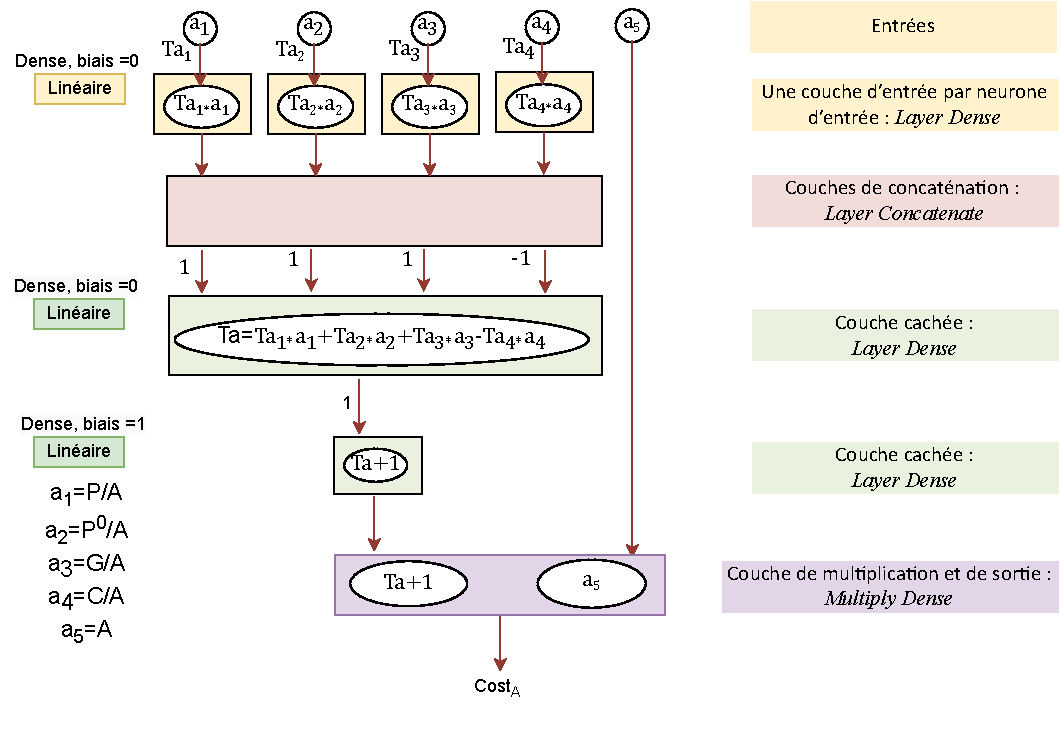
\includegraphics[height=11cm]{images_these/im_1_PROD_cost_value.pdf}}
	\caption[Réseau de neurones prédisant le coût $Cost_A$]{Réseau de neurones prédisant le coût $Cost_A$.}
	\label{1_PROD_cost_value}
\end{figure}

\begin{figure}[H]
	\centerline{
		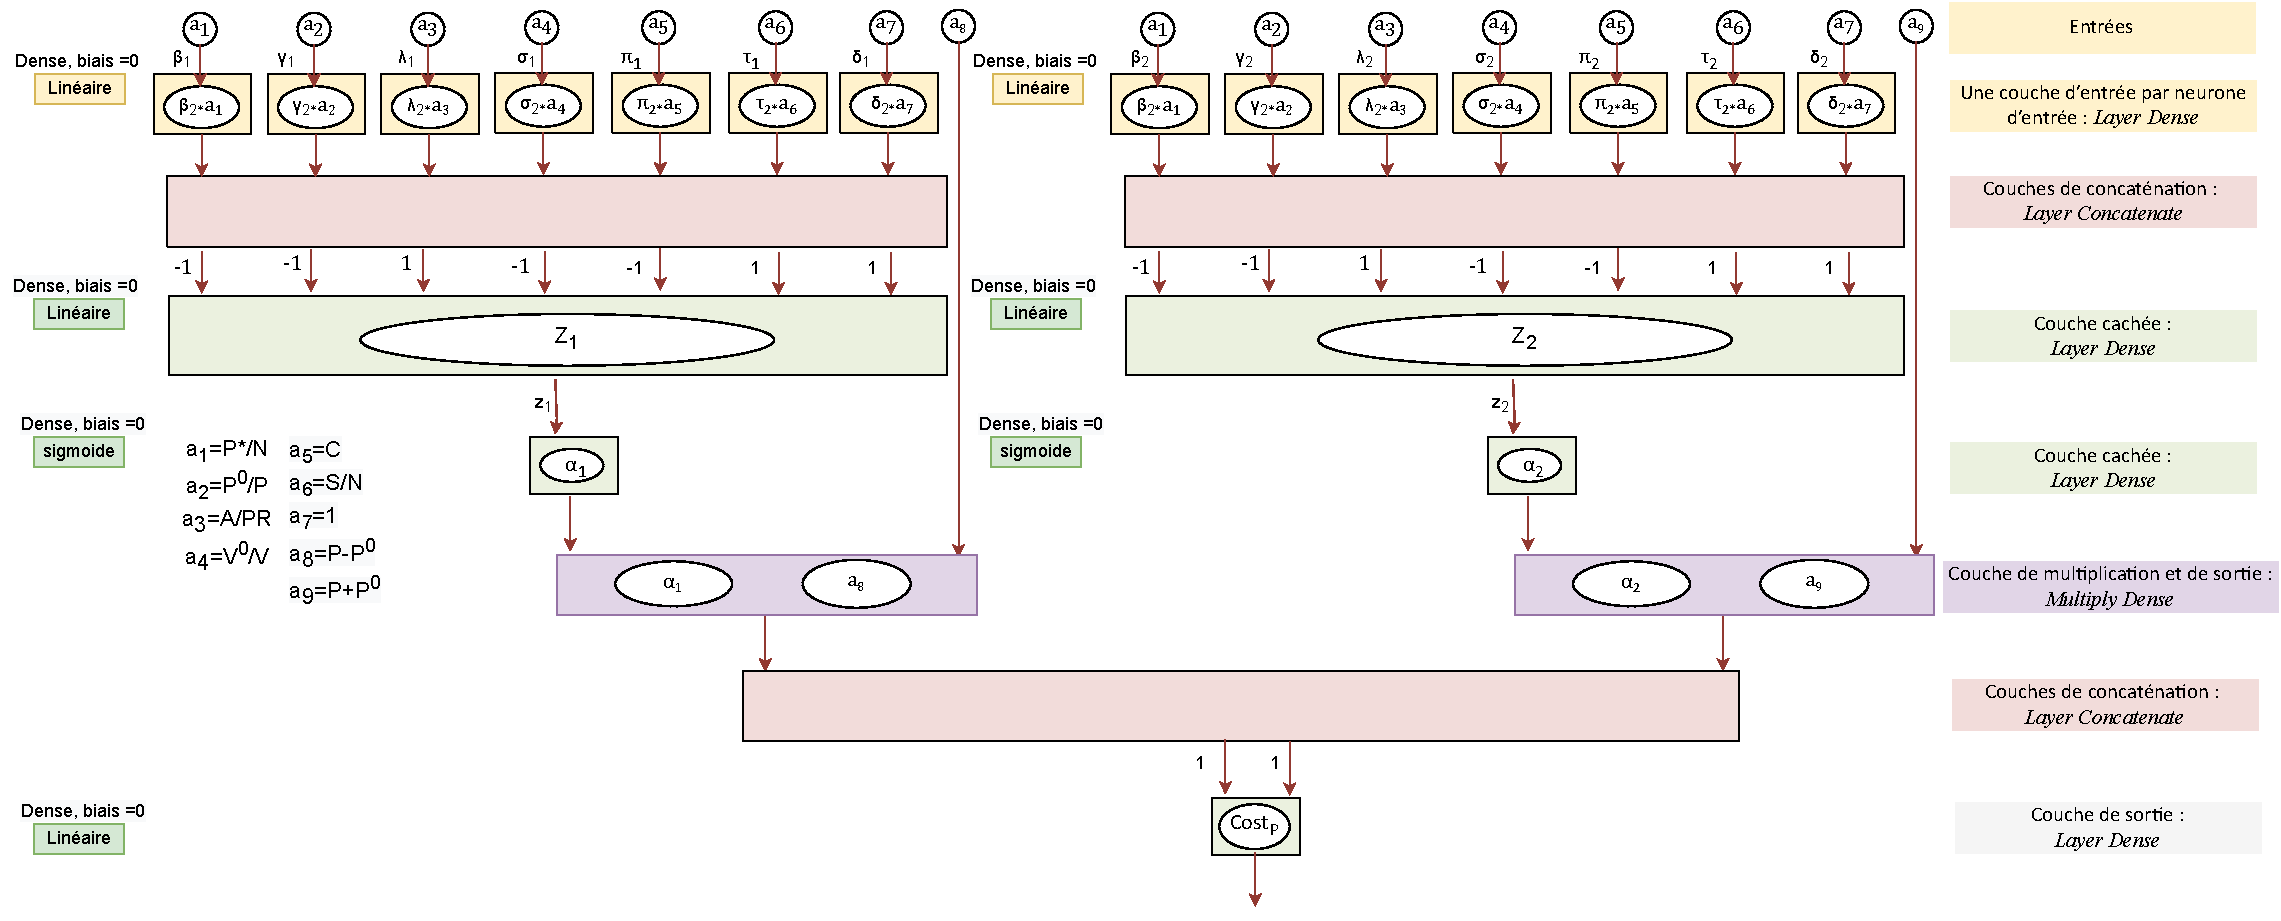
\includegraphics[height=8cm]{images_these/im_2_PROD_cost_value.pdf}}
	\caption[Réseau de neurones prédisant le coût $Cost_P$]{Réseau de neurones prédisant le coût  $Cost_P$.}
	\label{2_PROD_cost_value}
\end{figure}


\begin{figure}[H]
	\centerline{
		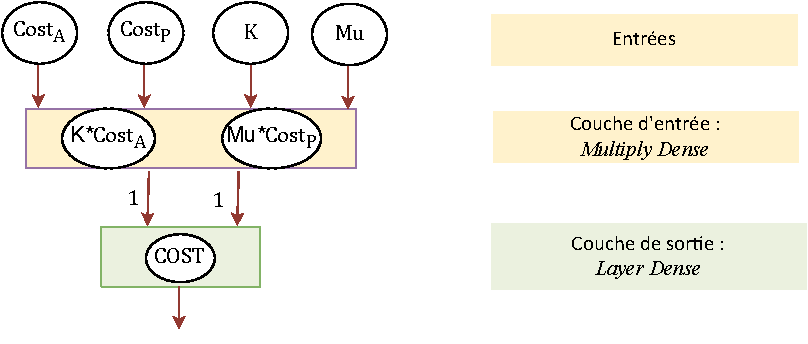
\includegraphics[height=5cm]{images_these/PROD_cost_value.pdf}}
	\caption[Réseau INDIC\_COUT prédisant le coût $COST$]{Réseau \textbf{INDIC\_COUT} prédisant le coût de production $COST$.}
	\label{PROD_cost_value}
\end{figure}


 Les fonctions d'activation utilisées sont la fonction sigmoide et la fonction linéaire.
Le nombre de poids et de biais du réseau de neurones \textbf{INDIC\_COUT} ne dépend pas de la taille des instances. L'algorithme d'optimisation utilisé est la descente de gradient stochastique. Les données de validation sont 1/3 des données d'apprentissage. Le nombre d'itérations correspondant à l'itération qui a fournit le plus petit gap sur les données de test est 201. La taille des batchs fixée ici est 32.  %La fonction de perte utilisé est lecarré des erreurs. 

Dans le réseau \textbf{INDIC\_COUT}, on a 20 poids à apprendre. 
\poubelle{
Les valeurs des poids après apprentissage sont : 
%\begin{itemize}[label=$\square$]
%\item $Ta_1=0,002325209323316812515$ ;
% \item $Ta_2=0,004769235383719205856$ ;
% \item  $Ta_3=0,003067760029807686806$ ;
% \item  $y=1$ ;
% \item  $Be_1=0,7660715579986572266$ ;
% \item  $Be_2=2,542258977890014648$ ;
% \item  $Be_0=2,634853363037109375$ ;
% \item  $z=1.087078332901000977$ ;
% \item  $Al_1=0,4537950754165649414$ ;
% \item  $Al_2=0,6376851201057434082$ ;
% \item  $Al_3=0,01474321633577346802$ ;
% \item  $Al_4=0,4492027759552001953$ ;
% \item  $Al_5=0$ ;
% \item  $Al_0=-1,560687541961669922$.
%\end{itemize}
\begin{itemize}[label=$\square$]
\item $Ta_1 = 0.00159026$
\item $Ta_2=0.00148414$
\item $Ta_3 = 0.00176206$
\item $Ta_4=0.4611397$
\item $\beta_1 =0.7780434 $
\item $ \gamma_1 =1.3931258 $
\item $\lambda_1 = 0.0066844$
\item $\sigma_1 =0 $
\item $\pi_1 = 0$
\item $ \tau_1= 3.6642723$
\item $ \delta_1= 0.00969145$
\item $\beta_2= 0.2616318$
\item $ \gamma_2= 1.5548283$
\item $\lambda_2 = 0.4804591$
\item $\sigma_2=0.68531483$
\item  $\pi_2=0$
\item $\tau_2= 1.8548965$
\item $ \delta_2=0.00457998$
\item$ z_1 = 2.4410741$
\item  $z_2 = 1.24242$
\end{itemize}
}
%%%%%%%%Le parcours du véhicule comme élément de decison
\subsubsection{Description des sorties du réseau de neurones \textbf{INDIC\_COUT}}
La sortie du réseau de neurones \textbf{INDIC\_COUT} est la valeur du coût de production $COST$.

\section{Expérimentations numériques}
\label{RN_exp}
Dans cette section dédiée aux expérimentations numériques, on va d'abord présenter les objectifs et le contexte technique de nos expériences. Ensuite, on présente les instances utilisées pour entrainer et tester nos réseaux. On finit cette section en présentant les résultats des tests effectués sur les réseaux présentés ci-dessus.
\subsection{Objectifs et contexte technique}

Ce que nous voulons ici, c'est obtenir une évaluation des performances des réseaux de neurones des figures (\ref{SFC}), (\ref{SFC2}), (\ref{FNFC}), (\ref{time_value_scheme}) et (\ref{PROD_cost_value}). Cela consiste à comparer les valeurs prédites par les réseaux aux valeurs optimales.

Les réseaux de neurones ont été implémentés en Python, sur un ordinateur fonctionnant sous le système d'exploitation Windows 10 avec un processeur IntelCore i5-6500@3.20 GHz, 16 Go de RAM et l'IDE utilisé est Visual Studio 2019. On a utilisé Tensorflow/Keras pour implémenter et manipuler nos réseaux de neurones. 

Les graphiques des gaps montrent la variation de l'erreur des données d'apprentissage et des données de test lorsqu'on fait varier le nombre d'itérations lors de la phase d'entraînement du réseau. La courbe rouge représente l'évolution de l'erreur calculée pour le groupe de test et la courbe bleue représente l'erreur calculée pour le groupe apprentissage. Nous ne montrerons pas ici la courbe des gaps des données de validation car elle n'est pas pertinente pour juger de la qualité de nos réseaux.


\subsection{Instances}

On a utilisé la procédure de génération d'instance décrite à la section (\ref{Gen_instance}) pour générer 6000 instances du problème SMEPC dont le nombre de périodes est égal à 20. Pour obtenir nos instances, on a élaboré un générateur d'instances. Les paramètres qu'on a utilisé pour générer aléatoirement nos instances sont :
\begin{enumerate}
	\item Concernant le nombre de stations, les instances peuvent être subdivisées en 4 catégories : les instances de 8 stations, celles de 10 stations, celles de 15 stations et celles de 20  stations. Le nombre de stations a été choisi arbitrairement.
	\item Concernant les coordonnées des stations, les instances peuvent être subdivisées en 3 catégories en fonction du carré dans lequel les coordonnées des instances sont sélectionnées aléatoirement : on a les instances dont les coordonnées de stations sont sélectionnées dans un carré $10\times 10$, celles sélectionnées dans un carré $20 \times 20$ et celles sélectionnées dans un carré $30 \times 30$.
	\item Concernant les coûts fixes et les coûts variables, on a décidé de générer ces coûts aléatoirement dans certains intervalles. Les instances ici peuvent être subdivisées en 5 catégories : 
	\begin{itemize}
		\item On a les instances dont le coût fixe est 5 et les coûts variables appartiennent à l'intervalle $[1,10]$. Pour cette catégorie d'instances même si le nombre de stations augmente, le coût de production aura du mal à augmenter car les coûts de production sont très petits ;
	    \item On a les instances dont le coût fixe est 50 et les coûts variables appartiennent à l'intervalle $[20,40]$ ;
	    \item On a les instances dont le coût fixe est 100 et les coûts variables appartiennent à l'intervalle $[20,40]$ ;
	    \item On a les instances dont le coût fixe est 100 et les coûts variables appartiennent à l'intervalle $[50,100]$ ;
	    \item On a les instances dont le coût fixe est 150 et les coûts variables appartiennent à l'intervalle $[50,100]$.
\end{itemize}
\end{enumerate} 
En croisant les critères 1, 2 et 3 ci-dessus, on obtient $4\times3\times5=60$ possibilités et pour chacune on génère 100 instances. Ce qui nous permet d'obtenir nos 6000 instances.

A partir de chaque instance, on calcule les valeurs des indicateurs qui serviront à avoir les valeurs utilisées comme entrées des réseaux de neurones. On récupère après exécution de l'algorithme Pipe-line VD\_PM du chapitre précédent pour chaque instance le numéro de période de la dernière opération de recharge et le coût de production. Ces données sont utilisées pour entrainer et tester nos réseaux de neurones. Les 6000 instances seront séparées en deux catégories d'instance à savoir les instances d'apprentissage qui nous serviront à entrainer les réseaux et les instances de test qui nous serviront à analyser le comportement de nos réseaux sur de nouvelles données. On décide d'avoir 90 instances de test et 5910 instances d'apprentissage. Pour avoir une idée des caractéristiques des instances utilisées, on fait une analyse statistique de nos instances. La section suivante est consacrée à présenter cette analyse.
%décrire les colonnes des instances


%\begin{figure}[H]
%	\centerline{
%		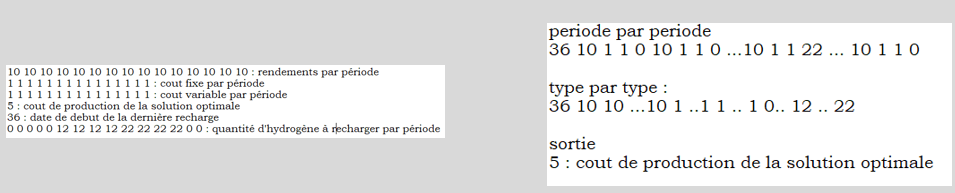
\includegraphics[height=4cm]{images_these/type_period_data.png}}
%	\caption[Pré-traitement des données]{Pré-traitement des données.}
%	\label{type_period_data}
%\end{figure}

%Dans la section suivante, on présente une analyse statistique de nos 6000 instances.

\subsubsection{Analyse statistique des instances}


%$M$ représente le nombre de stations, $\#instances$ représente le nombre d'instance, $N$ représente le nombre de périodes et $\#recharges$ représente le nombre de recharge. De cette analyse statistique, on constate que le nombre de stations est compris entre 6 et 14. On constate qu'on a plus de 1400 instances de 6 stations. On a plus de 800 instances de 8 stations, on a moins de 200 instances de 10 stations. On a moins de 100 instances de 12 stations et moins de 50 instances de 50 stations. De plus, on constate que le nombre de périodes est compris entre 8 et 80, la majorité des instances ont entre 12 et 40 périodes. Concernant le nombre de recharge, on constate qu'il est compris entre 2 et 8. On a plus de 800 instances de 4 recharges. On a plus de 700 instances de 3 recharges. On a plus de 500 instances de 5 recharges. On a moins de 200 instances  de 2 recharges. On a moins de 200 instances de 6 recharges et on a moins de 50 instances de 7 et 8 recharges.

%\begin{figure}
%	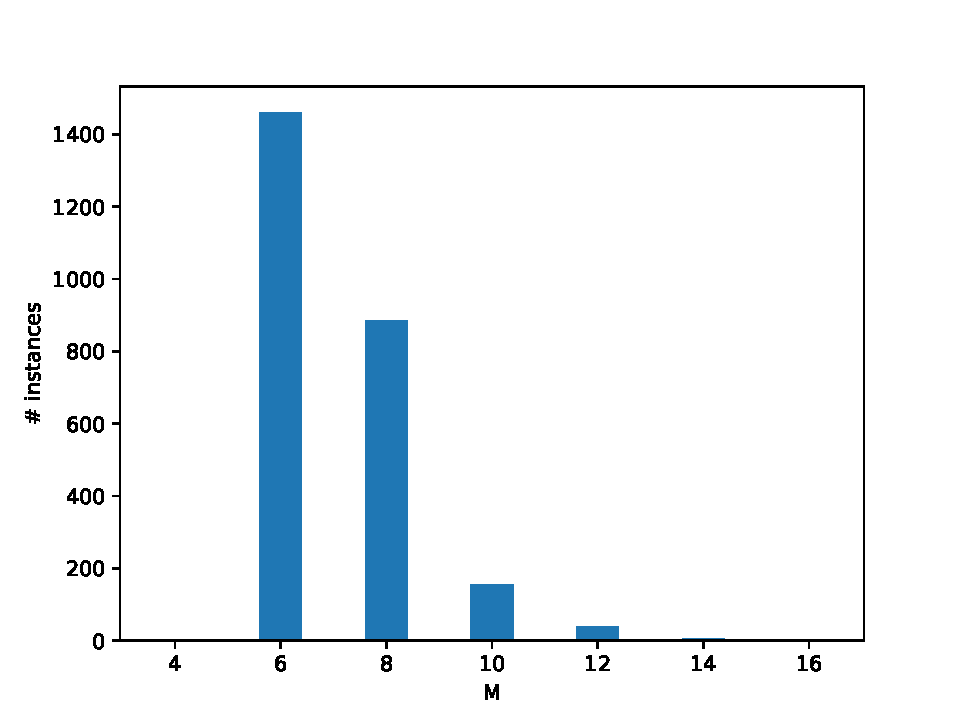
\includegraphics[width=9cm]{images_these/2500_CourbeM.pdf}\hfill
%	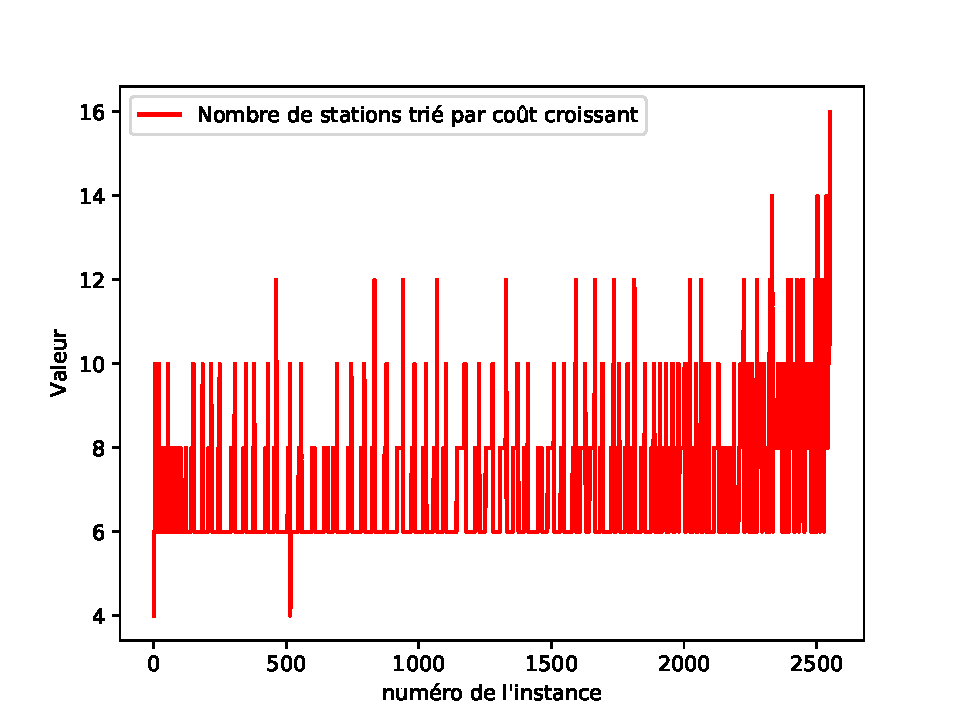
\includegraphics[width=9cm]{images_these/2500_Stats_instances_Nbstations.pdf}
%	\caption{Nombre de stations ($M$)}\label{periode_station}
%\end{figure}
%
%\begin{figure}
%	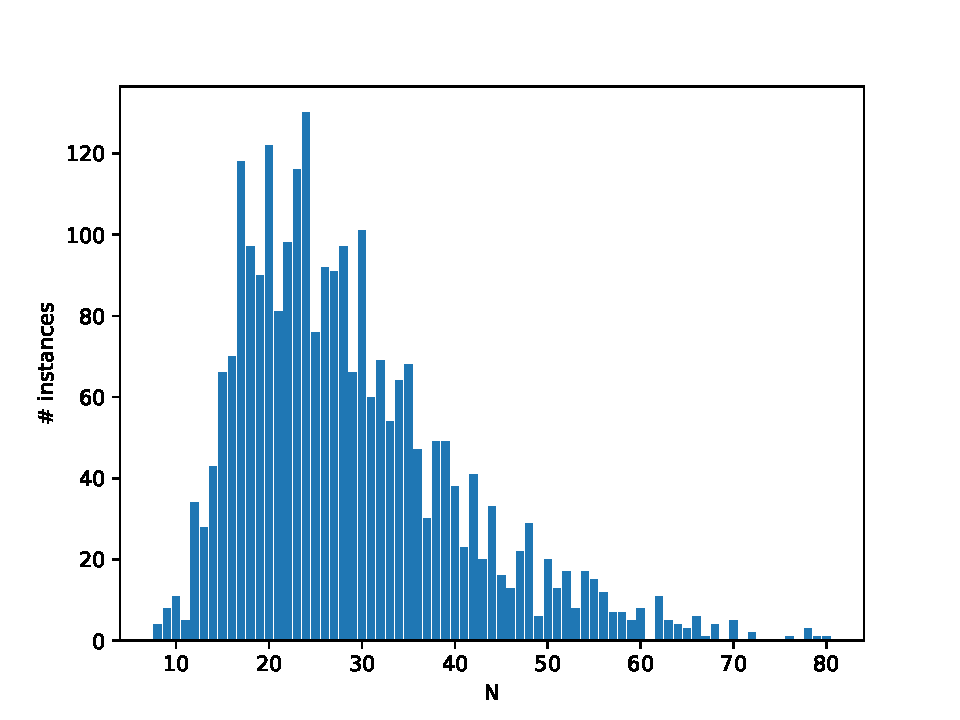
\includegraphics[width=9cm]{images_these/2500_CourbeN.pdf}\hfill
%	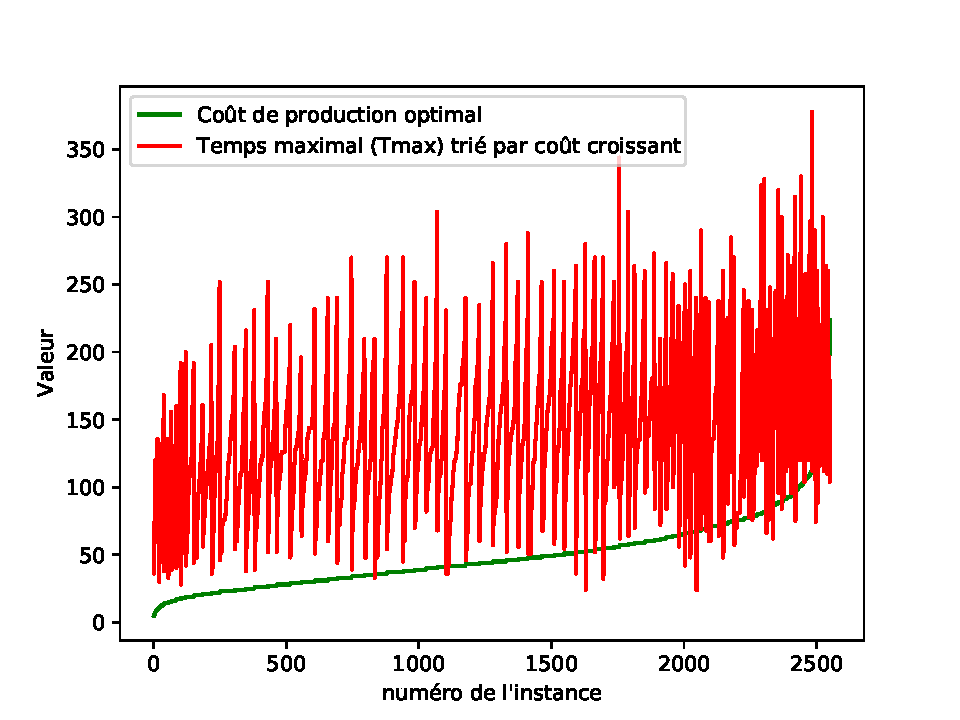
\includegraphics[width=9cm]{images_these/2500_Stats_instances_Tmax.pdf}
%	\caption{Nombre de périodes ($N$) et ($TMAX$)}\label{periode_stats}
%\end{figure}
%
%\begin{figure}
%		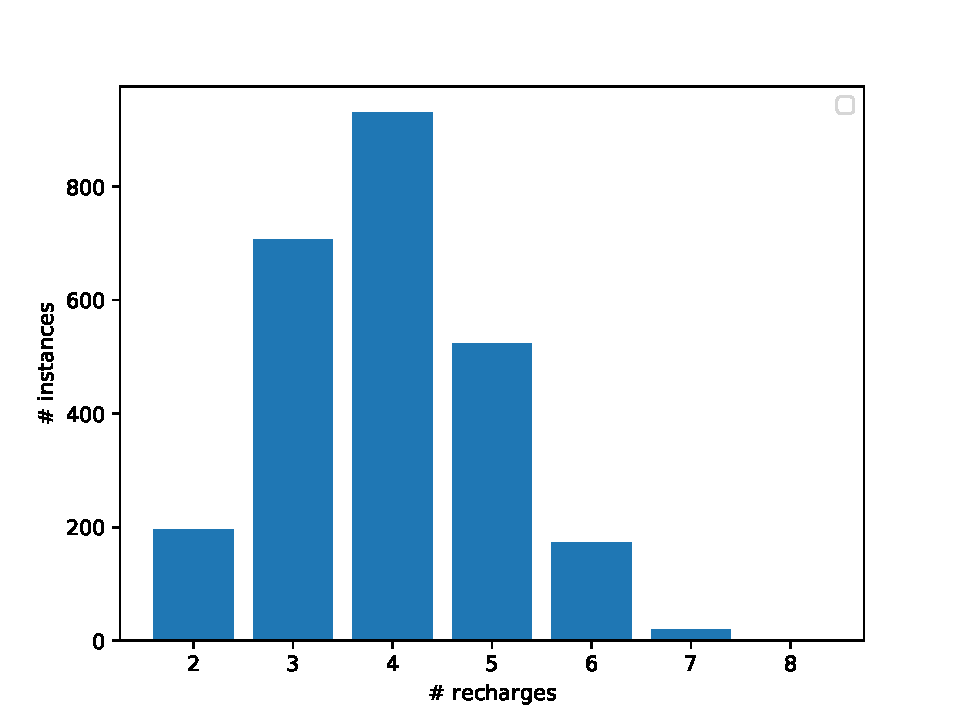
\includegraphics[width=9cm]{images_these/2500_Nombre_dinstance_par_nb_recharge.pdf}\hfill
%	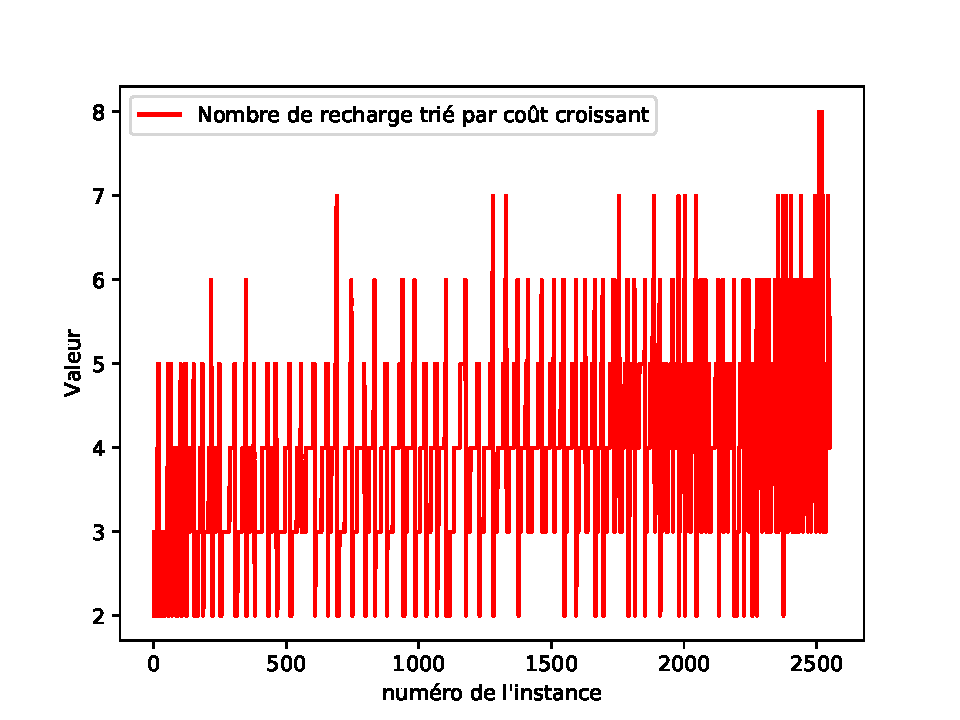
\includegraphics[width=9cm]{images_these/2500_Stats_instances_Nbrecharge.pdf}
%	\caption{Nombre de recharge de nos instances}\label{recharge}
%\end{figure}
%
%\begin{figure}
%		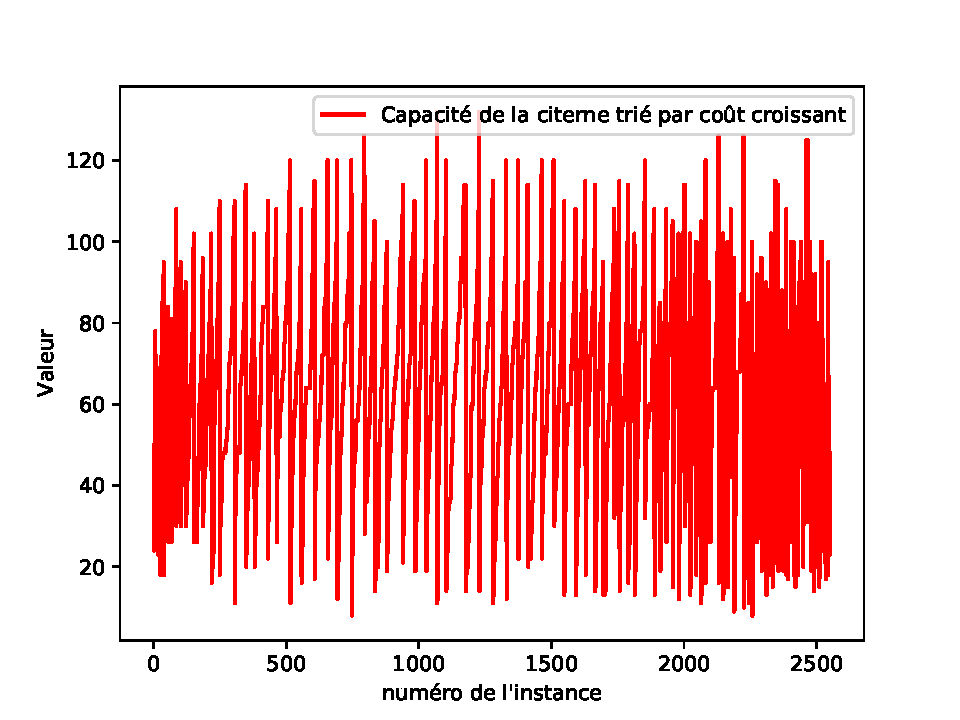
\includegraphics[width=9cm]{images_these/2500_Stats_instances_citerne.pdf}\hfill
%	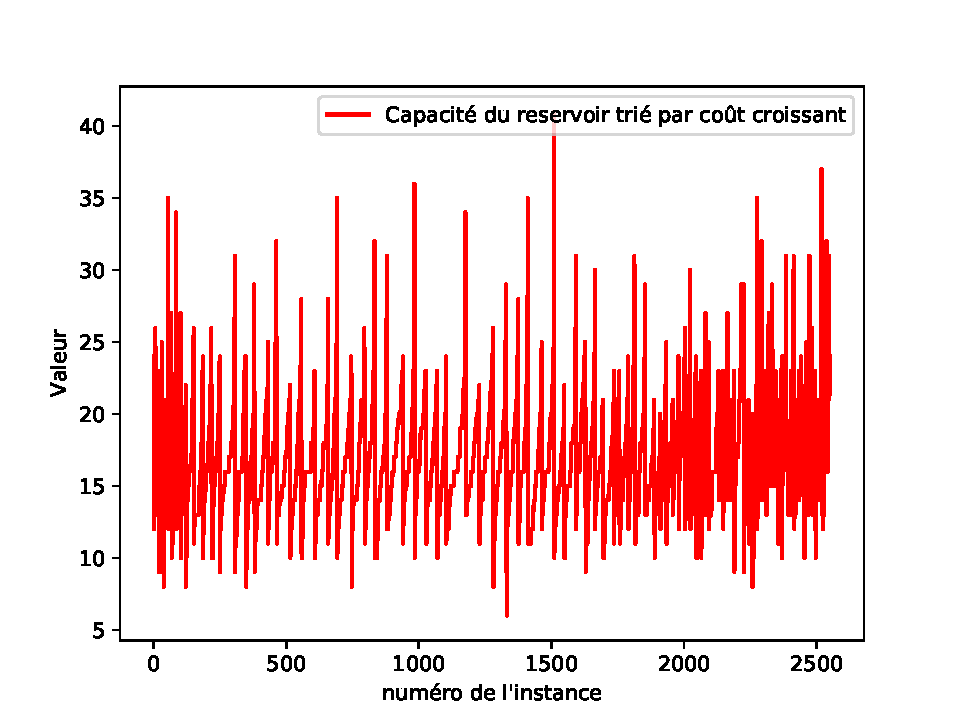
\includegraphics[width=9cm]{images_these/2500_Stats_instances_reservoir.pdf}
%	\caption{Capacité}\label{capacité}
%\end{figure}
%
%\begin{figure}
%		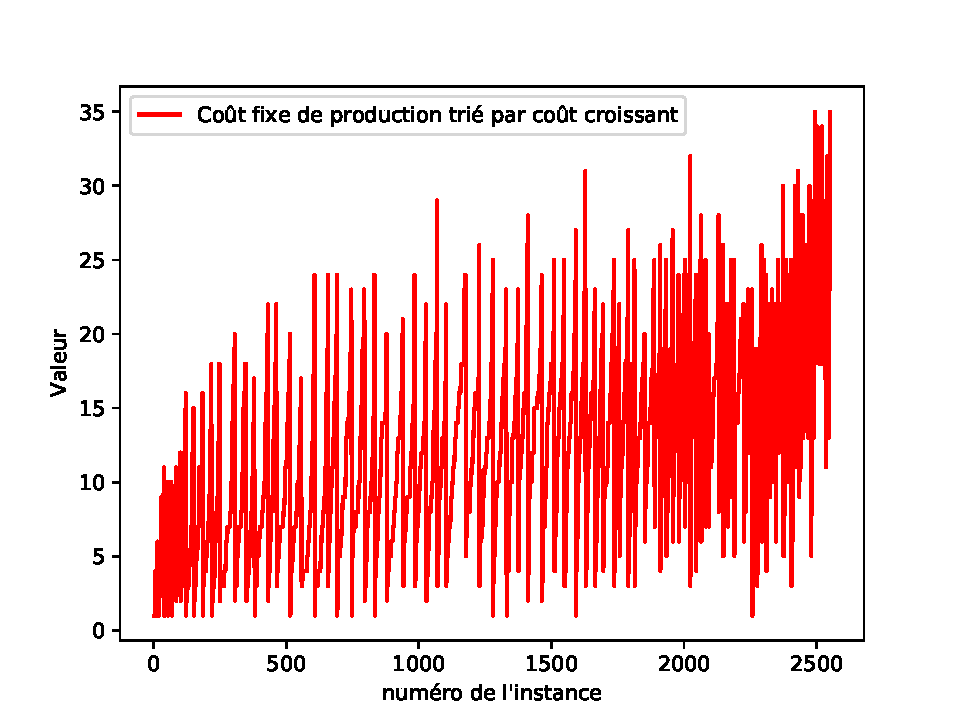
\includegraphics[width=9cm]{images_these/2500_Stats_instances_coutfix.pdf}\hfill
%	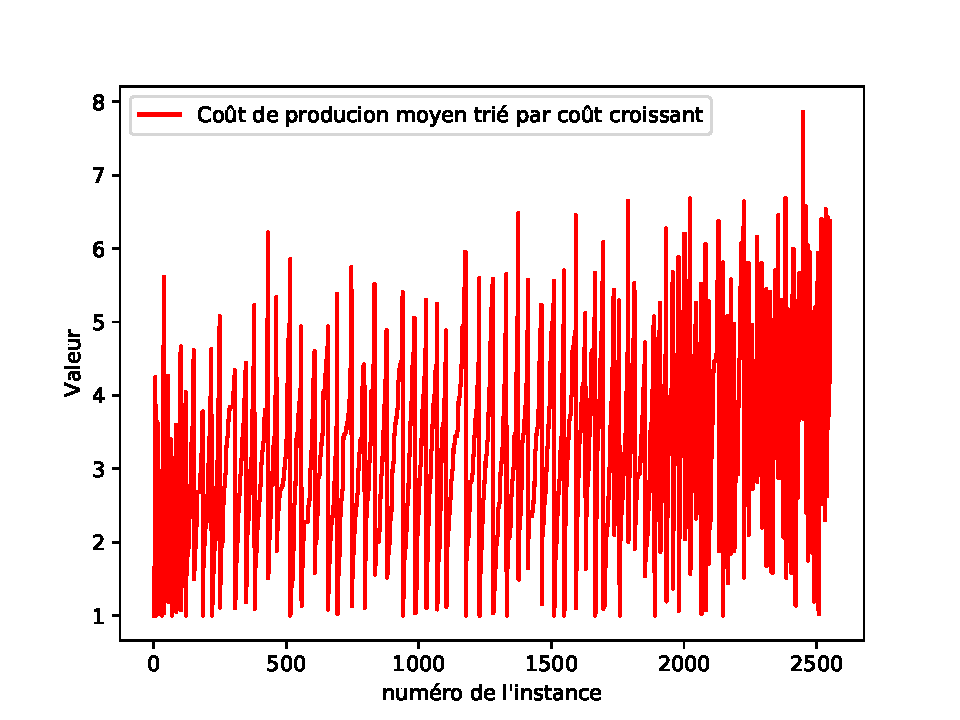
\includegraphics[width=9cm]{images_these/2500_Stats_instances_cout_var.pdf}
%	\caption{Coût fixe et coût variable}\label{cout}
%\end{figure}



%\begin{figure}
%	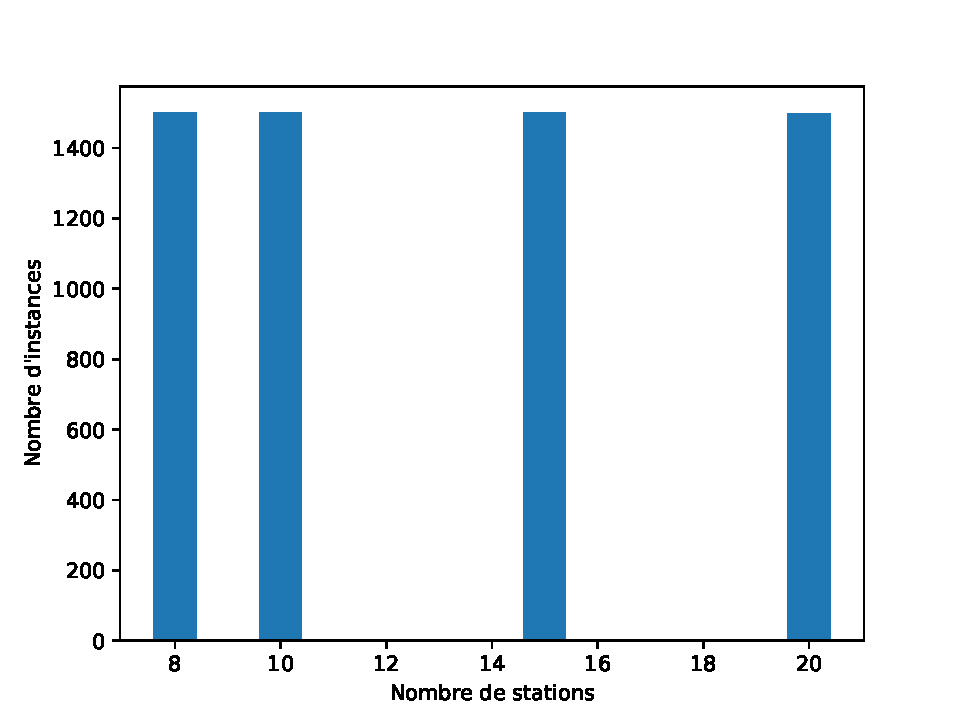
\includegraphics[width=9cm]{images_these/6000_CourbeM.pdf}\hfill
%	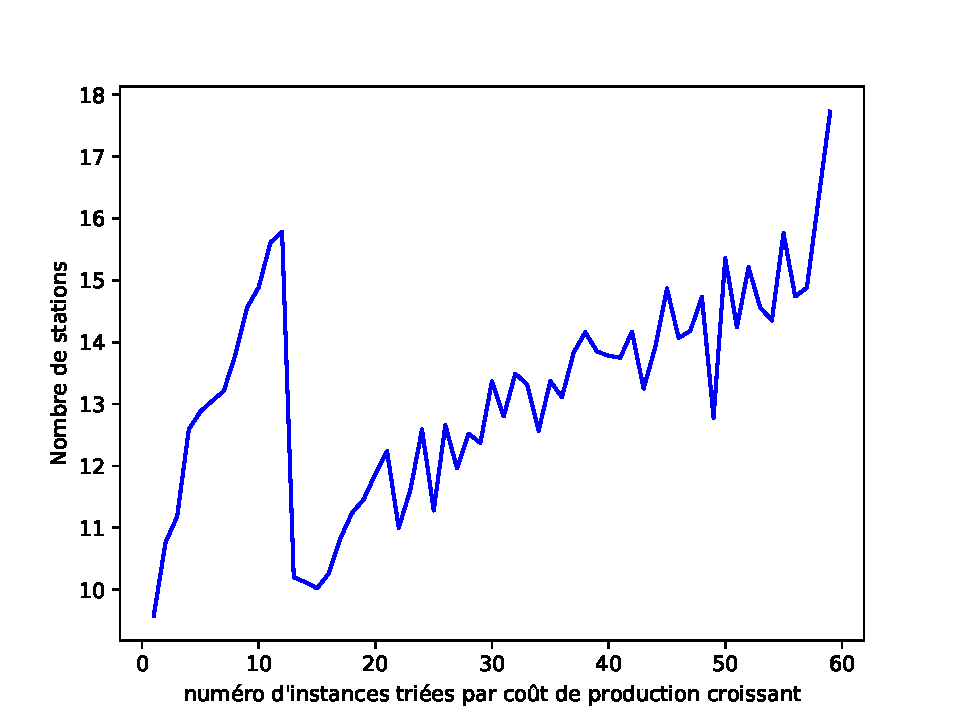
\includegraphics[width=9cm]{images_these/6000_Stats_instances_Nbstations.pdf}
%	\caption{Nombre de stations ($M$)}\label{6000_periode_station}
%\end{figure}
%\begin{figure}
%	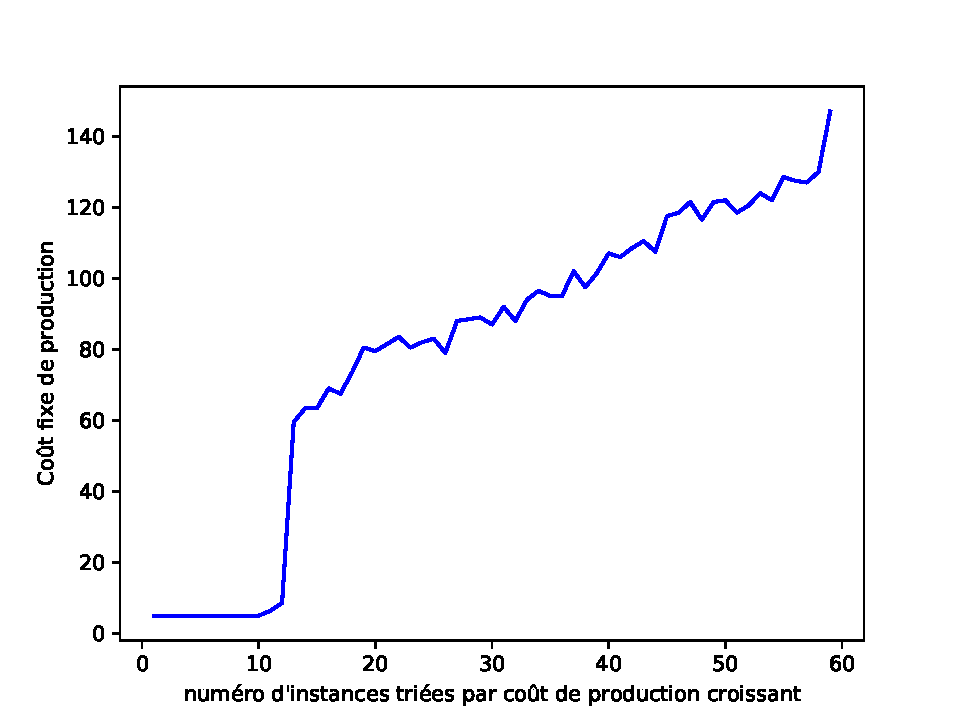
\includegraphics[width=9cm]{images_these/6000_Stats_instances_coutfix.pdf}\hfill
%	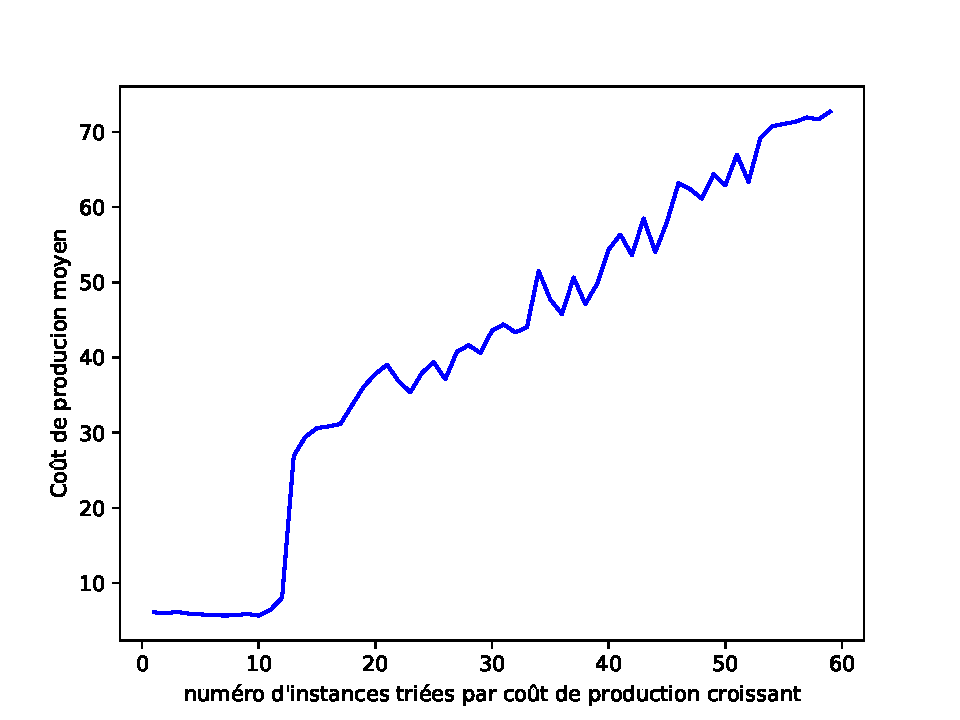
\includegraphics[width=9cm]{images_these/6000_Stats_instances_cout_var.pdf}
%	\caption{Coût fixe et coût variable}\label{6000_cout}
%\end{figure}


%\begin{figure}
%		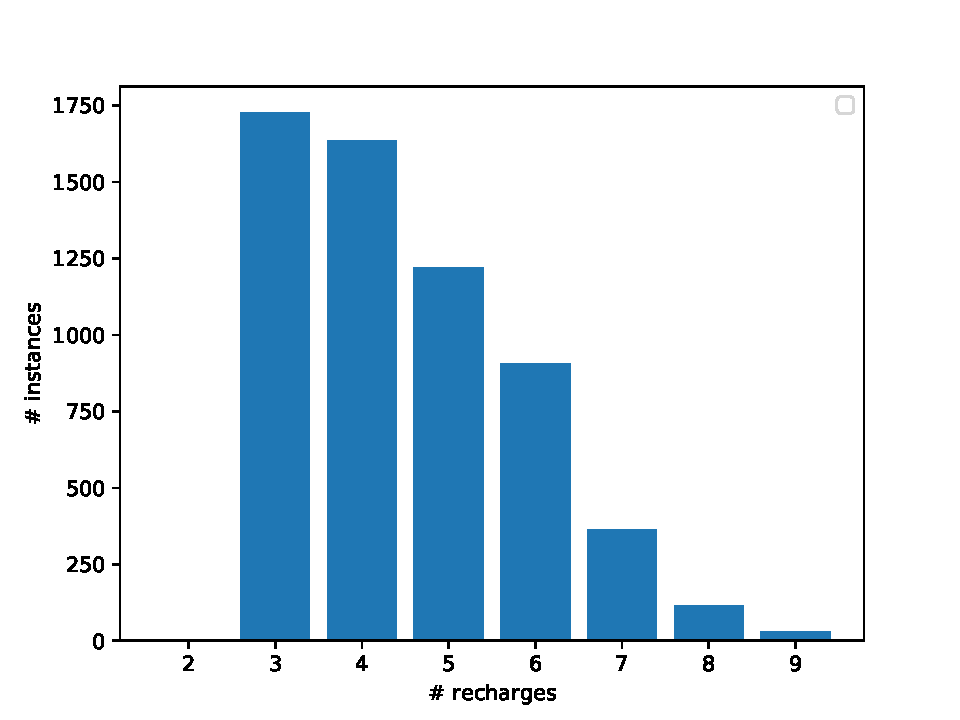
\includegraphics[width=9cm]{images_these/6000_Nombre_dinstance_par_nb_recharge.pdf}\hfill
%	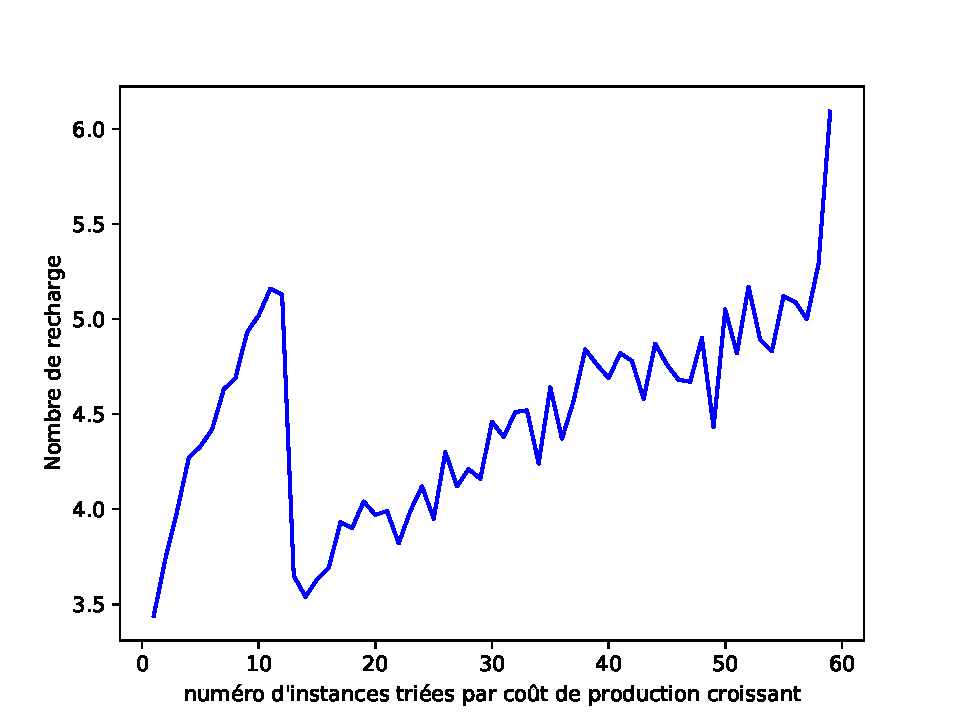
\includegraphics[width=9cm]{images_these/6000_Stats_instances_Nbrecharge.pdf}
%	\caption{Nombre de recharge de nos instances}\label{6000_recharge}
%\end{figure}

%\begin{figure}
%		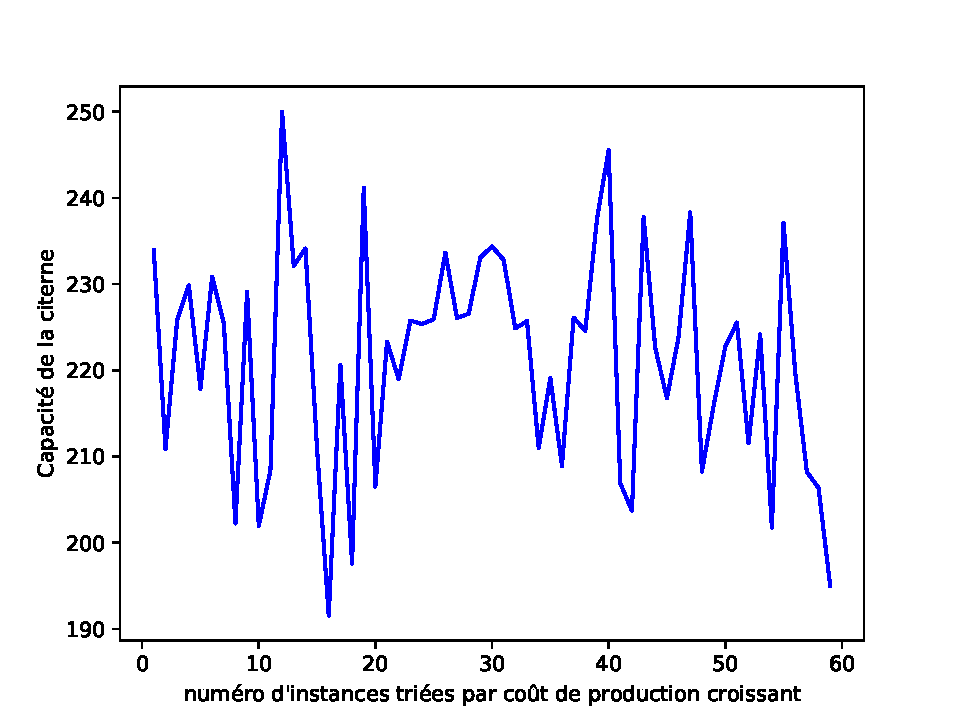
\includegraphics[width=9cm]{images_these/6000_Stats_instances_citerne.pdf}\hfill
%	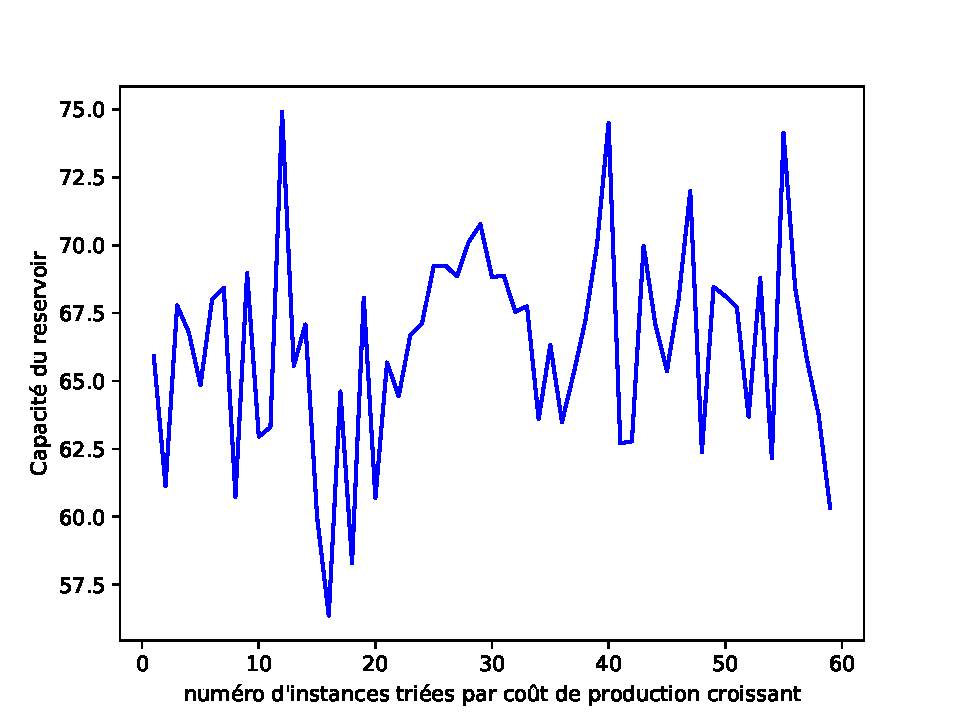
\includegraphics[width=9cm]{images_these/6000_Stats_instances_reservoir.pdf}
%	\caption{Capacité}\label{6000_capacité}
%\end{figure}
Les figures (\ref{6000_periode_station}), (\ref{6000_recharge}), (\ref{6000_periode_stats}), (\ref{6000_cout}) et (\ref{6000_capacité}) illustrent l'analyse statistique des instances. Par souci de lisibilité de nos figures, on n'affiche pas les instances une par une mais on affiche la moyenne de chaque paquet de 100 instances. On ordonne préalablement nos instances par coût de production croissant.  Les instances générées avec le coût  fixe 5 et les coûts variables appartenant à l'intervalle $[1,10]$ ont des coûts tellement petits que le nombre de stations n'impacte pas trop le coût d'où les pics observés sur les figures (\ref{6000_periode_station}) (b), (\ref{6000_recharge}) (b), (\ref{6000_periode_stats}) (b)

La figure (\ref{coutprod}) représente le coût moyen de production regroupé par paquets de 100 instances. Sachant que toutes les instances ont préalablement été ordonnées par coût de production croissant. On constate que les coûts de production de nos instances sont compris entre 0 et 2000.
\begin{figure}[H]
	\centerline{
		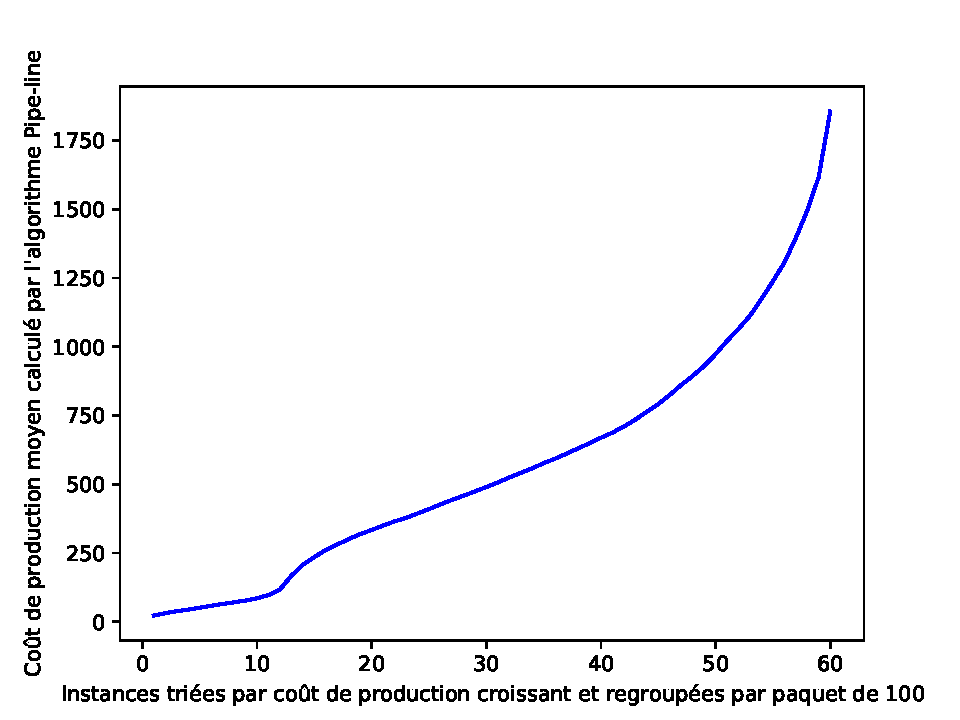
\includegraphics[width=9cm]{images_these/Stats_instances_coutopt.pdf}}
	%		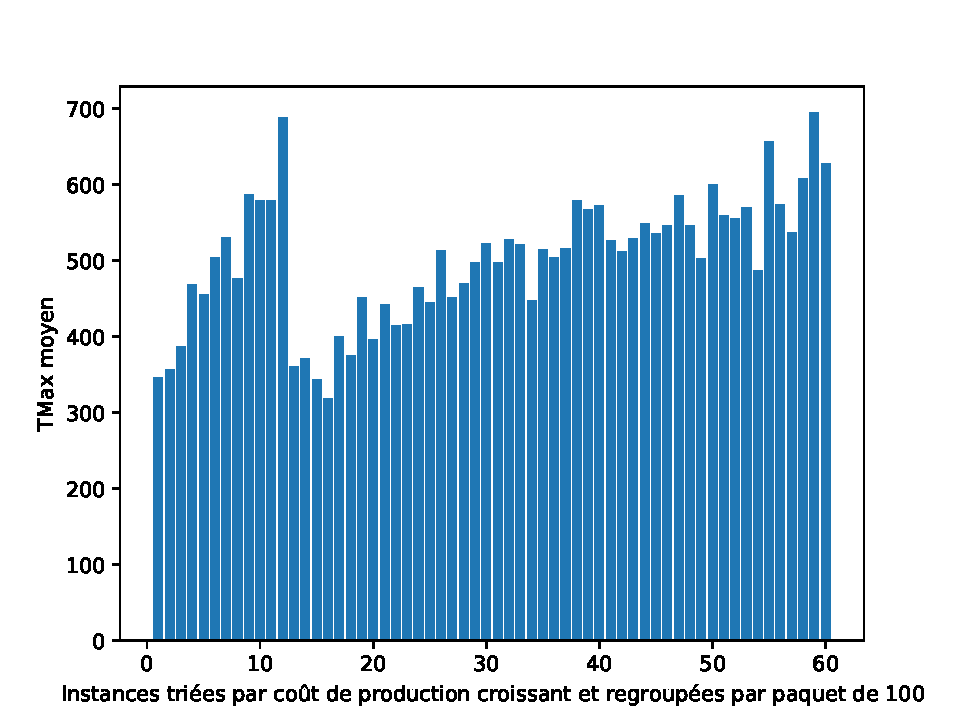
\includegraphics[width=9cm]{images_these/Stats_instances_Tmax.pdf}}
	\caption[Coût moyen de production par ordre croissant et regroupé par paquet de 100 instances]{ Coût moyen de production par ordre croissant et regroupé par paquet de 100 instances. Ce coût a été obtenu en exécutant l'algorithme Pipe-line VD\_PM du chapitre précédent. }\label{coutprod}
\end{figure}

La figure \ref{6000_cout}(a) représente le coût fixe moyen de production regroupé par paquet de 100 instances. La figure \ref{6000_cout}(a) représente le coût variable moyen de production regroupé par paquet de 100 instances. Sachant que toutes les instances ont préalablement été ordonnées par coût de production croissant. De ces figures, on peut dire que le coût de production croit lorsque le cout fixe et le coût variable croient aussi. Ce qui montre que ces coûts peuvent être utilisés comme entrées des réseaux qui prédisent le coût de production.
\begin{figure}[H]
	\centering
	\begin{tabular}{c c}
		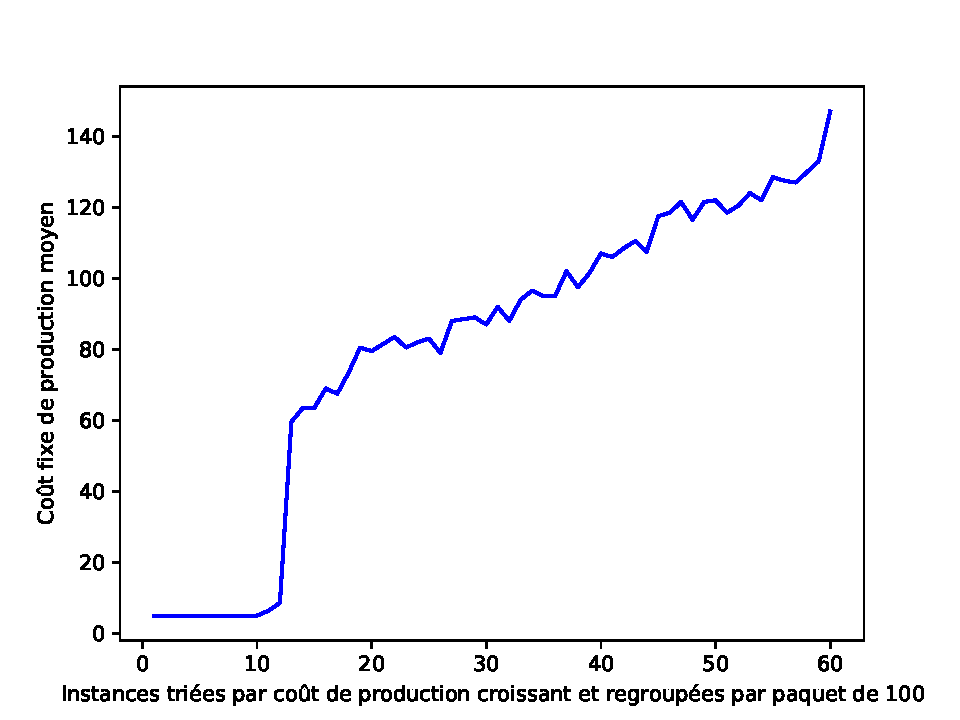
\includegraphics[width=9cm]{images_these/Stats_instances_coutfix.pdf} &
		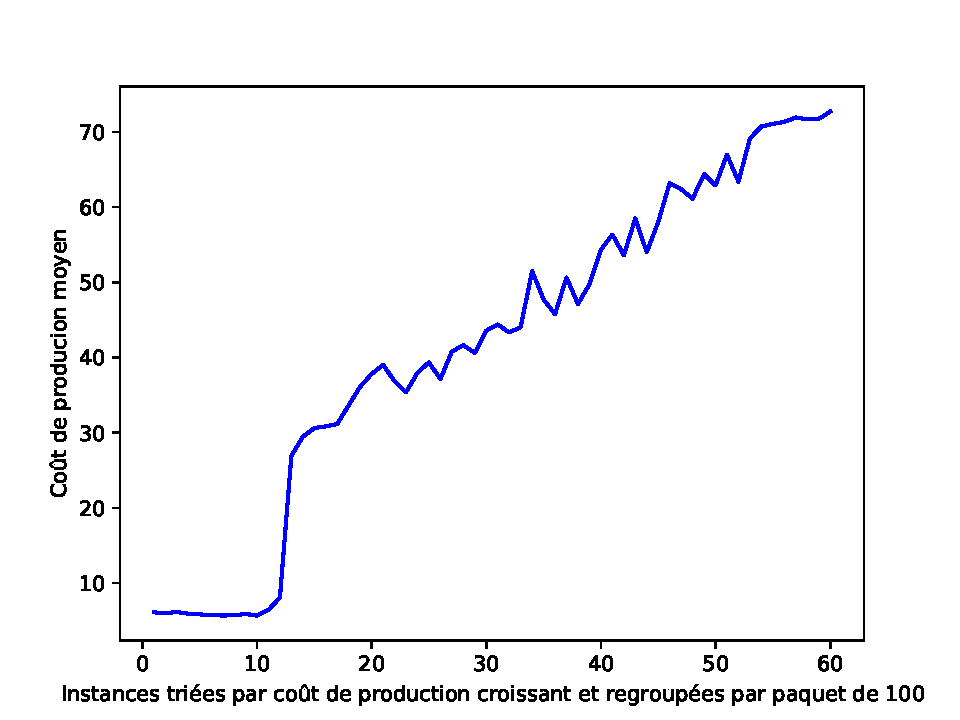
\includegraphics[width=9cm]{images_these/Stats_instances_cout_var.pdf}
		\\
		(a) & (b)
	\end{tabular}
	\caption[Coût fixe moyen et coût variable moyen de production regroupé par paquet de 100 instances]{La figure (a) représente le coût fixe moyen de production regroupé par paquet de 100 instances. La figure (b) représente le coût variable moyen de production regroupé par paquet de 100 instances. Sachant que les instances ont préalablement été classées par coût de production croissant.}\label{6000_cout}
\end{figure}

La figure (\ref{6000_periode_station})(a) représente le nombre d'instances par nombre de stations. On constate qu'on a 1500 instances de 8 stations, 1500 instances de 10 stations, 1500 instances de 15 stations et 1500 instances de 20 stations. La figure (\ref{6000_periode_station})(b) représente la moyenne du nombre de stations regroupé par paquet de 100 instances. On constate que du paquet d'instances 1 au paquet d'instances 12, le nombre de stations croit au fur et à mesure que le coût de production croit. Mais à partir du paquet d'instances 13  on a une brusque chute du nombre de stations moyen malgré le fait que le coût augmente. Ceci est dû au fait qu'à la génération des instances, on a crée des instances avec un coût fixe très petit 5, alors que les autres coûts sont au moins quatre fois plus élevés. On peut conclure que le nombre de stations n'est pas une valeur pertinente à utiliser pour prédire le coût de production.
%plus on a de stations plus le coût croit
\begin{figure}[H]
	\centering
	\begin{tabular}{c c}
		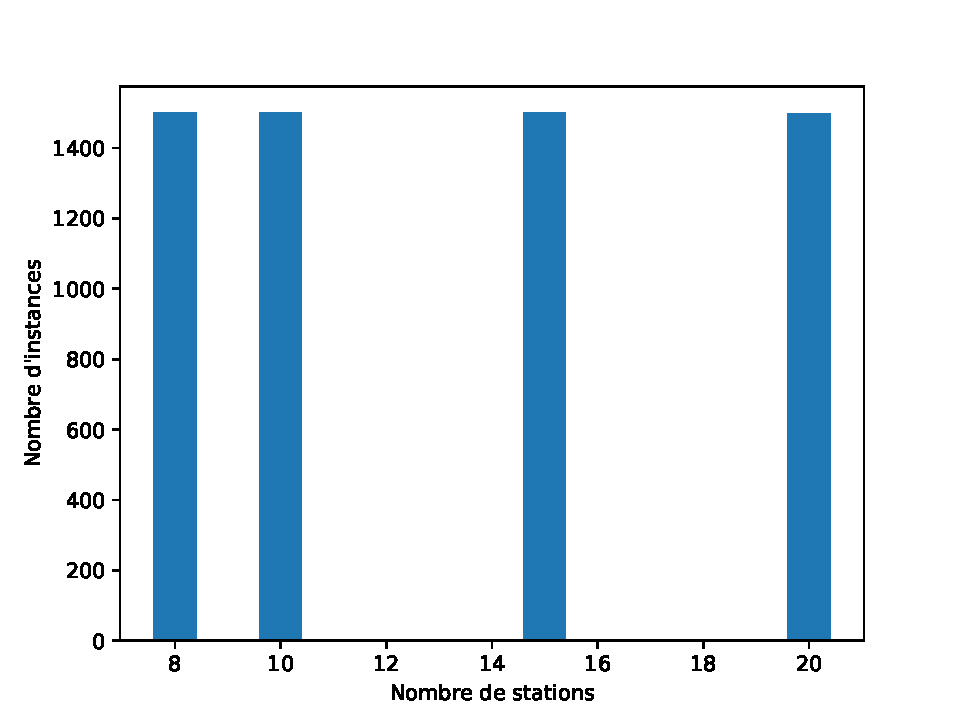
\includegraphics[width=9cm]{images_these/CourbeM.pdf} &
		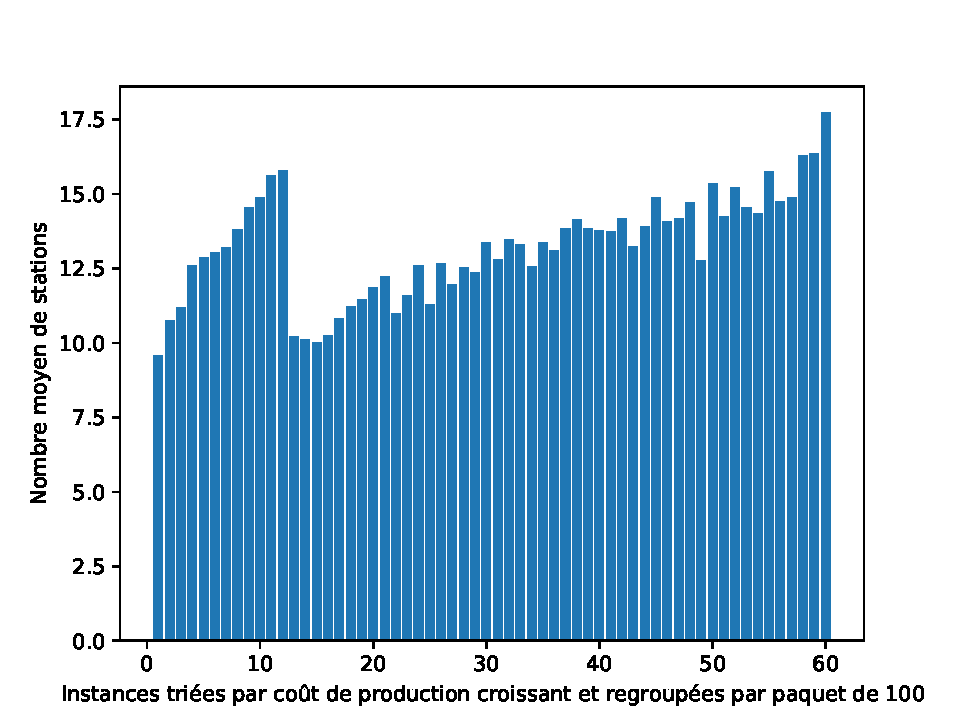
\includegraphics[width=9cm]{images_these/Stats_instances_Nbstations.pdf}
		\\
		(a) & (b)
	\end{tabular}
	\caption[Moyenne du nombre de stations regroupé par paquet de 100 instances]{La figure (a) représente le nombre d'instances par nombre de stations. La figure (b) représente la moyenne du nombre de stations regroupé par paquet de 100 instances. Sachant que les instances ont été classées par coût de production croissant. }\label{6000_periode_station}
\end{figure}

 On a exécuté l'algorithme DPS\_VD du chapitre précédent pour obtenir la stratégie de recharge réduite. La figure (\ref{6000_recharge})(a) représente le nombre d'instances par nombre de recharges. On constate que la majorité des instances ont entre 4 et 6 recharge. La figure (\ref{6000_recharge})(b) représente la moyenne du nombre de recharges regroupé par paquet de 100 instances. Sachant que toutes les instances ont préalablement été ordonnées par coût de production croissant. On constate que du paquet d'instances 1 au paquet d'instances 12, le nombre moyen de recharges croit au fur et à mesure que le coût de production croit. Mais à partir du paquet d'instances 13  on a une brusque chute du nombre moyen de recharges malgré le fait que le coût augmente. Ceci est dû au fait qu'à la génération des instances, on a crée des instances avec un coût fixe très petit 5, alors que les autres coûts sont au moins quatre fois plus élevés. On peut conclure que le nombre moyen de recharges n'est pas une valeur pertinente à utiliser pour prédire le coût de production.

\begin{figure}[H]
	\centering
	\begin{tabular}{c c}
		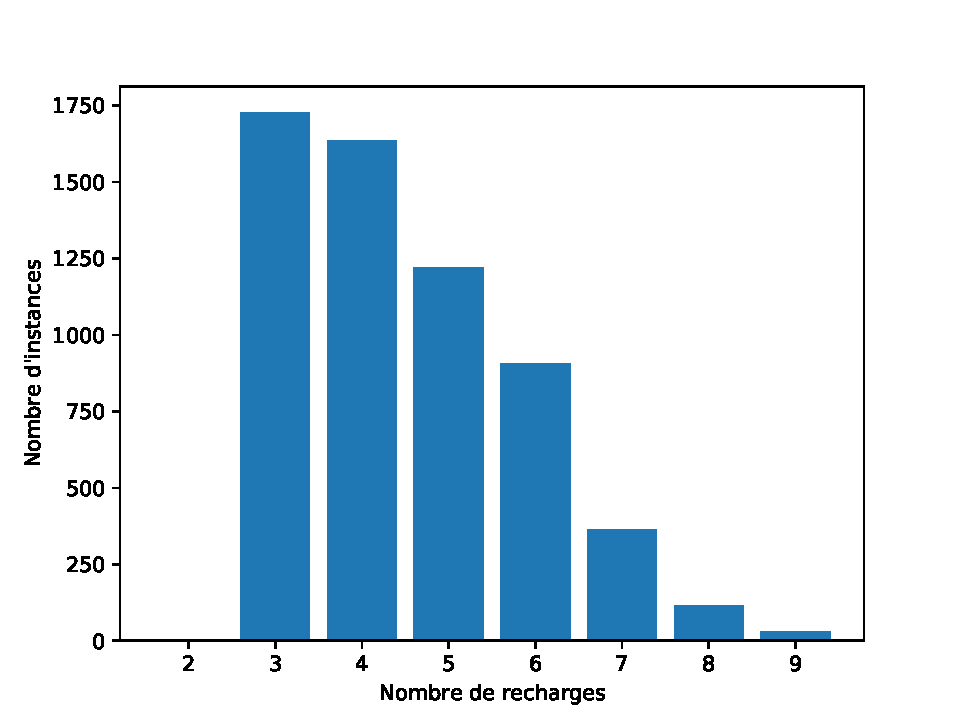
\includegraphics[width=9cm]{images_these/Nombre_dinstance_par_nb_recharge.pdf} &
		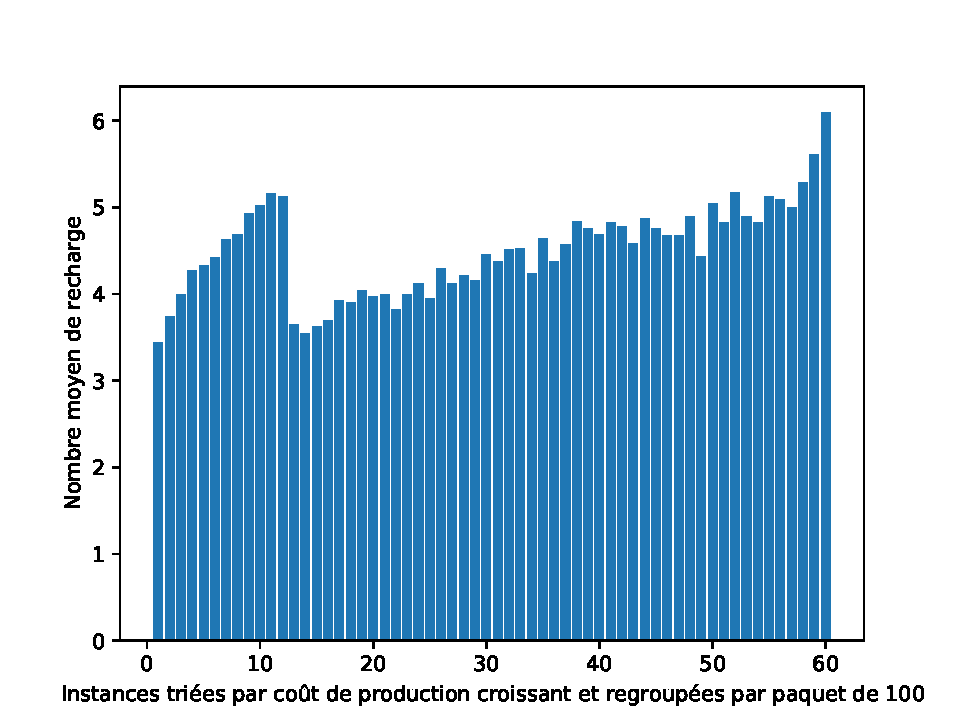
\includegraphics[width=9cm]{images_these/Stats_instances_Nbrecharge.pdf}
		\\
		(a) & (b)
	\end{tabular}
	\caption[Moyenne du nombre de recharges regroupé par paquet de 100 instances]{La figure (a) représente le nombre d'instances par nombre de recharges. La figure (b) représente la moyenne du nombre de recharges regroupé par paquet de 100 instances. Sachant que les instances ont été classées par coût de production croissant. }\label{6000_recharge}
\end{figure}

La figure (\ref{6000_periode_stats}) (a) représente la durée moyenne d'une période de production regroupé par paquet de 100 instances. Sachant que toutes les instances ont préalablement été ordonnées par coût de production croissant.
La figure (\ref{6000_periode_stats}) (b) représente l'évolution du temps maximal moyen ($TMax$) regroupé par paquet de 100 instances. Sachant que toutes les instances ont préalablement été ordonnées par coût de production croissant. On peut conclure que la durée moyenne d'une période et le temps maximal moyen ne sont pas des valeurs pertinentes à utiliser pour prédire le coût de production.
\begin{figure}[H]
	\centering
	\begin{tabular}{c c}
		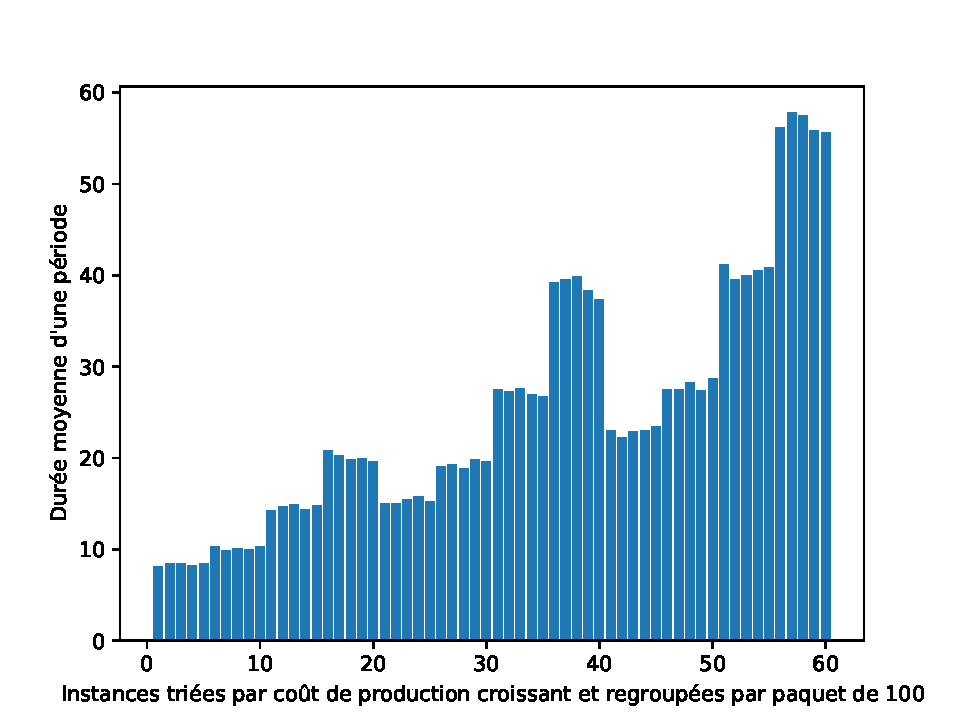
\includegraphics[width=9cm]{images_these/Stats_instances_P.pdf} &
		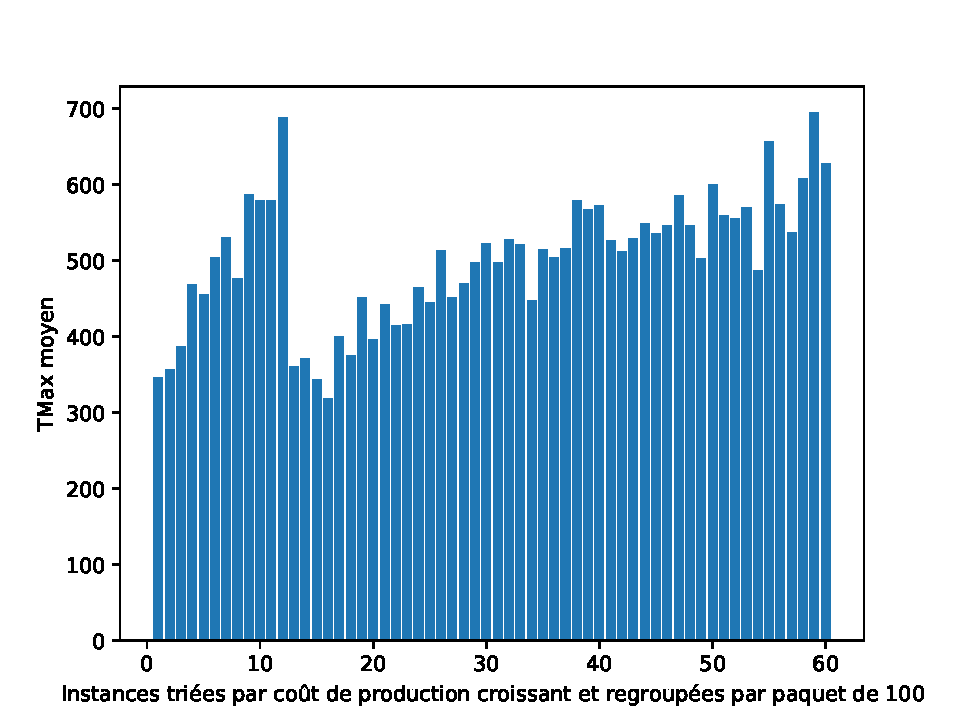
\includegraphics[width=9cm]{images_these/Stats_instances_Tmax.pdf}
		\\
		(a) & (b)
	\end{tabular}
	\caption[Évolution du temps maximal moyen regroupé par paquet de 100 instances]{La figure (a) représente la durée moyenne d'une période de production regroupé par paquet de 100 instances. La figure (b) représente l'évolution du temps maximal moyen regroupé par paquet de 100 instances. Sachant que les instances ont été classées par coût de production croissant. }\label{6000_periode_stats}
\end{figure}


La figure (\ref{6000_capacité})(a) représente la capacité moyenne de la citerne regroupé par paquet de 100 instances. La figure (\ref{6000_capacité})(a) représente la capacité moyenne du réservoir regroupé par paquet de 100 instances. Sachant que les instances ont été classées par coût de production croissant. On peut conclure que la capacité moyenne de la citerne et la capacité moyenne du réservoir ne sont pas des valeurs pertinentes à utiliser pour prédire le coût de production.

\begin{figure}[H]
	\centering
	\begin{tabular}{c c}
		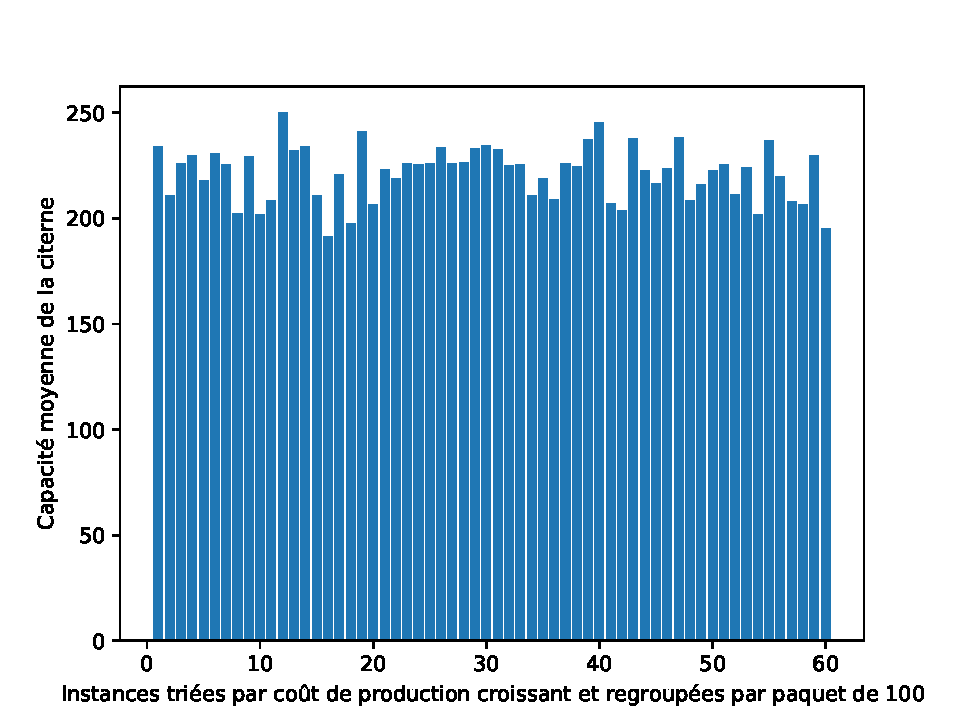
\includegraphics[width=9cm]{images_these/Stats_instances_citerne.pdf} &
		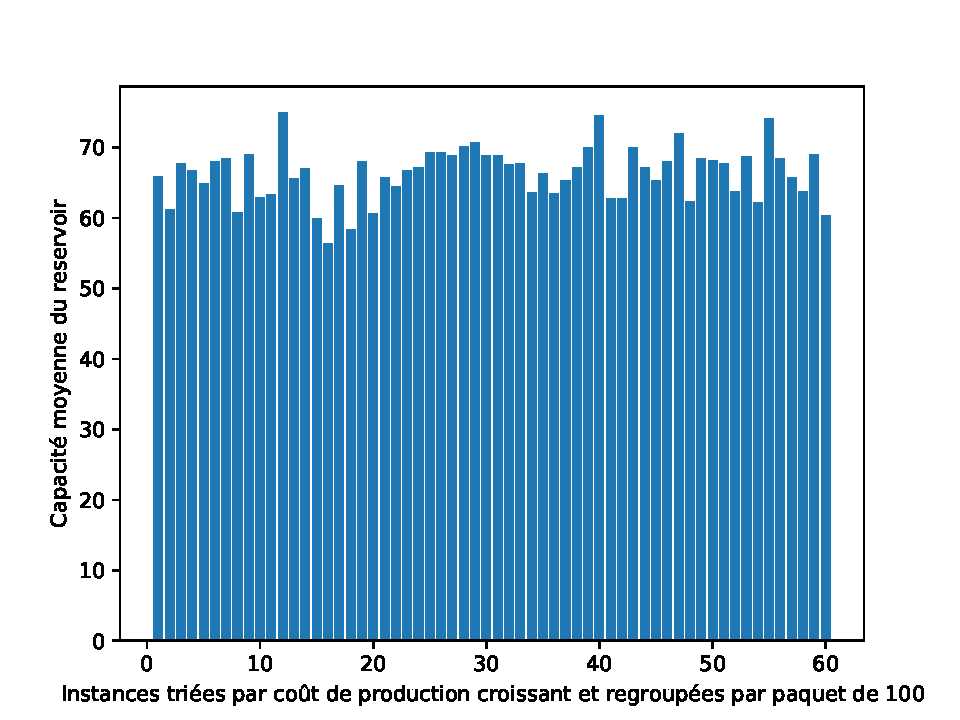
\includegraphics[width=9cm]{images_these/Stats_instances_reservoir.pdf}
		\\
		(a) & (b)
	\end{tabular}
	\caption[Capacité moyenne du réservoir et de la citerne regroupé par paquet de 100 instances]{La figure (a) représente la capacité moyenne de la citerne regroupé par paquet de 100 instances. La figure (a) représente la capacité moyenne du réservoir regroupé par paquet de 100 instances. Sachant que les instances ont été classées par coût de production croissant.}\label{6000_capacité}
\end{figure}


%\subsubsection{Analyse en composantes principales (ACP) des instances}
%L'analyse en composantes principales permet de visualiser un jeu de données ayant un très grand nombre de dimensions. Une dimension ici étant une variable (colonnes) des données. L'ACP synthétise ces variables en seulement quelques nouvelles variables appelées \textbf{composantes principales}. Ce qui réduit donc le nombre de dimensions du jeu de données. Ces nouvelles variables sont une combinaison linéaire des variables d'origine. Le nombre de nouvelles variables est alors inférieur au nombre de variables d'origine. L'inconvénient de cette technique est une possible perte d'information à cause de la réduction de dimension. Cette technique est habituellement utilisée lorsque les variables sont fortement corrélées.
%La figure (\ref{PCA}) présente le résultat de l'analyse en composantes principales de nos instances.
%\begin{figure}
%	\centerline{
%		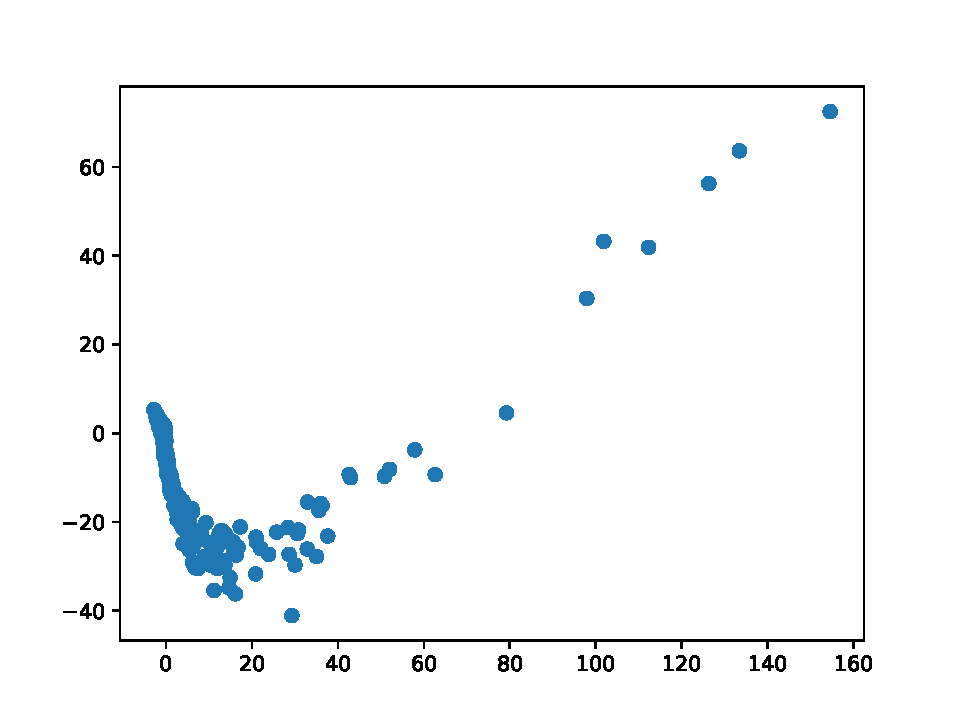
\includegraphics[width=9cm]{images_these/Analyse_PCA_2549.pdf}}
%	\caption{Analyse ACP de nos instances}\label{PCA}
%\end{figure}

%\subsection{Pertinence des indicateurs}
%Les figures (\ref{Indicateurs_energie}), (\ref{Indicateurs_free}), (\ref{Indicateurs_time}), (\ref{Indicateurs_time_G}), (\ref{Indicateurs_unit}), (\ref{Indicateurs_absolute}) représentent les valeurs des indicateurs pour 2460 instances d'apprentissage et 90 instances de test. L'axe des abscisses représente le numéro des instances et l'axe des ordonnées représente la valeur de l'indicateur.
%Les variables de ces figures ont la signification suivante :
%la valeur Ind $Mu$ est la valeur de l'indicateur $Mu$ ;
%la valeur Ind $K$ est la valeur de l'indicateur $K$ ;
%la valeur Ind $R$ est la valeur de l'indicateur $R$ ;
%la valeur $Opt$ est la somme du numéro de période de la dernière recharge et du coût de production de la solution optimale ;
%la valeur Ind $C$ est la valeur de l'indicateur $C$ ;
%la valeur Ind $C^*$ est la valeur de l'indicateur $C^*$ ;
%la valeur Ind $R^*$ est la valeur de l'indicateur $R^*$ ;
%la valeur Ind $P^*$ est la valeur de l'indicateur $P^*$ ;
%la valeur Ind $V^*$ est la valeur de l'indicateur $V^*$ ;
%la valeur Ind $A^*$ est la valeur de l'indicateur $A^*$ ;
%la valeur Ind $Delta$ est la valeur de l'indicateur $De$ ;
%la valeur Ind $G^*$ est la valeur de l'indicateur $G^*$ ;
%la valeur Ind $P$ est la valeur de l'indicateur $P$ ;
%la valeur Ind $P0$ est la valeur de l'indicateur $P^0$ ;
%la valeur Ind $G$ est la valeur de l'indicateur $G$ ;
%la valeur Ind $G0$ est la valeur de l'indicateur $G^0$ ;
%la valeur Ind $A$ est la valeur de l'indicateur $A$ ;
%la valeur Ind $A0$ est la valeur de l'indicateur $A^0$ ;
%la valeur Ind $V$ est la valeur de l'indicateur $V$ ;
%la valeur Ind $V0$ est la valeur de l'indicateur $V^0$.
%
%\begin{figure}
%	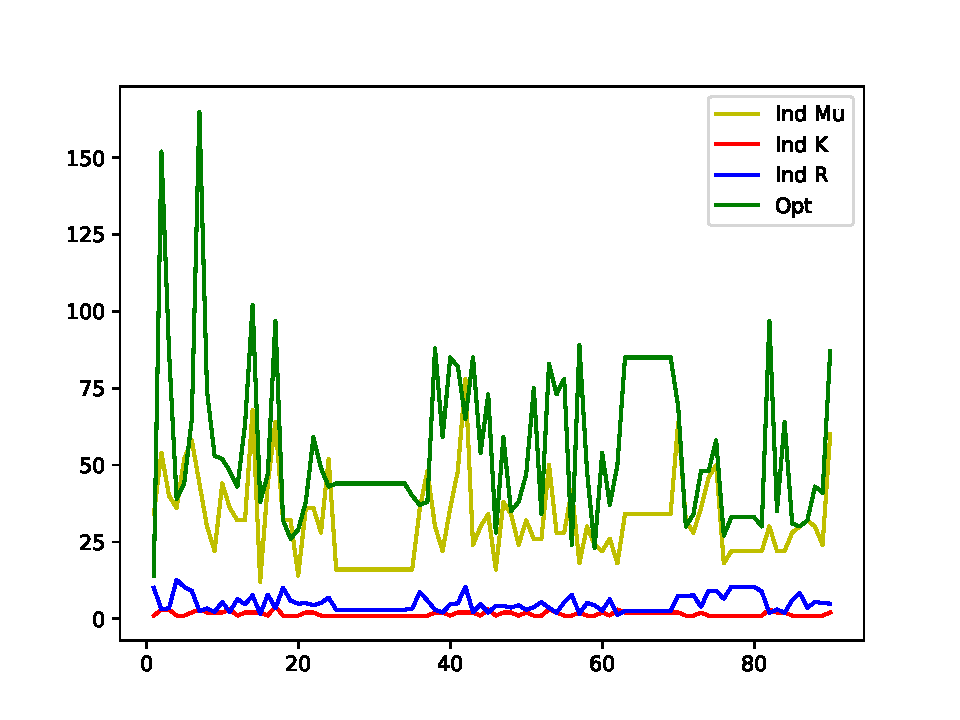
\includegraphics[width=9cm]{images_these/Indicateurs_energie_90.pdf}\hfill
%	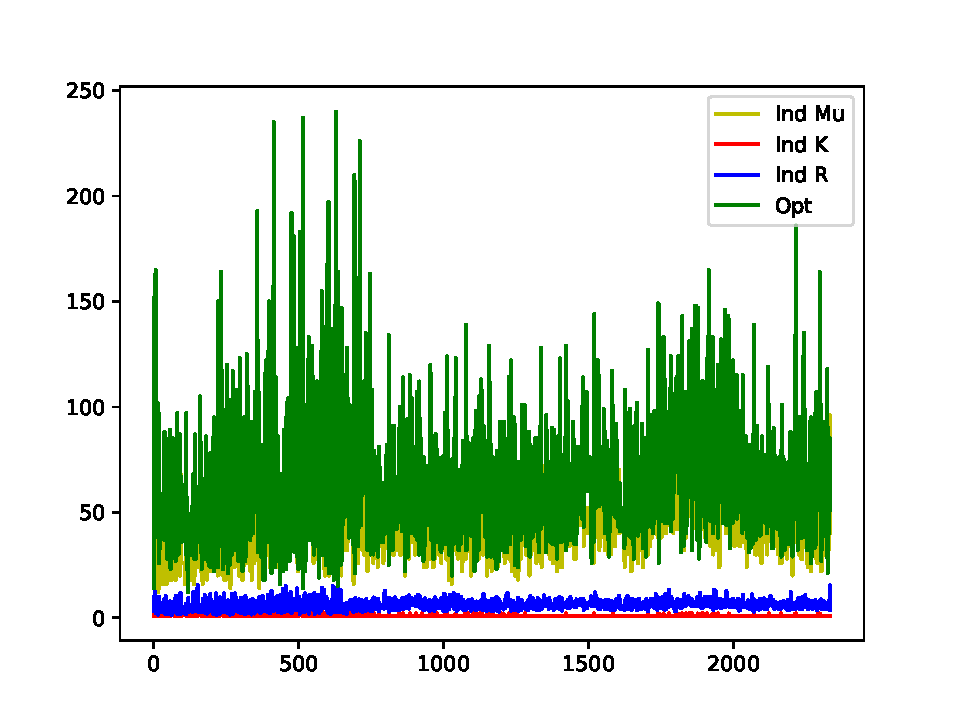
\includegraphics[width=9cm]{images_these/Indicateurs_energie.pdf}
%	\caption{Indicateurs énergétiques}\label{Indicateurs_energie}
%\end{figure}
%
%\begin{figure}
%	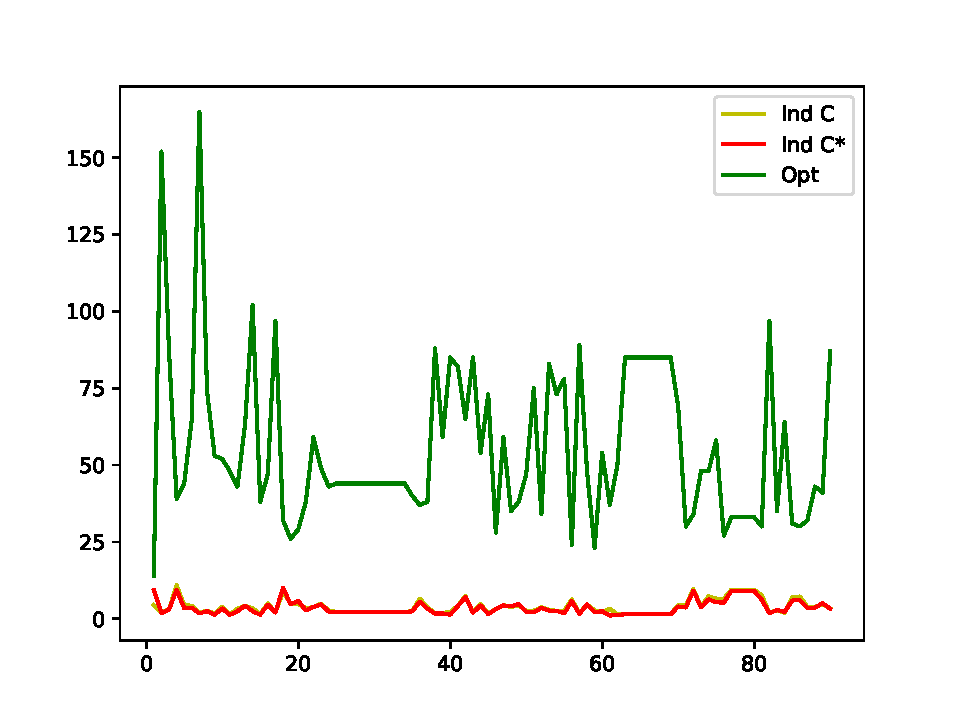
\includegraphics[width=9cm]{images_these/Indicateurs_free_90.pdf}\hfill
%	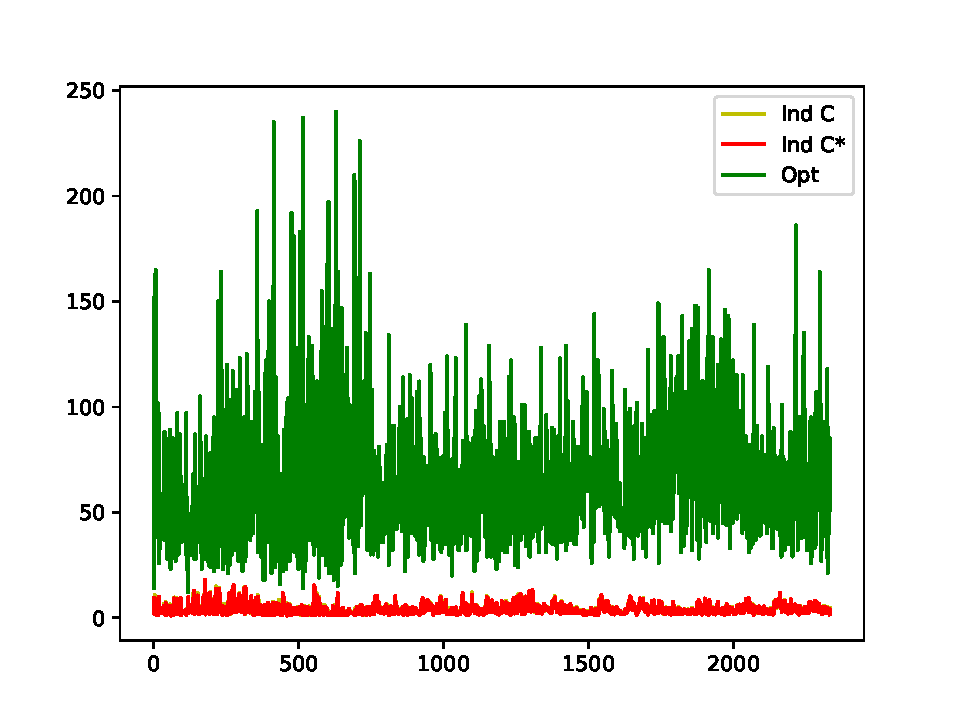
\includegraphics[width=9cm]{images_these/Indicateurs_free.pdf}
%	\caption{Indicateurs libres}\label{Indicateurs_free}
%\end{figure}
%
%\begin{figure}
%	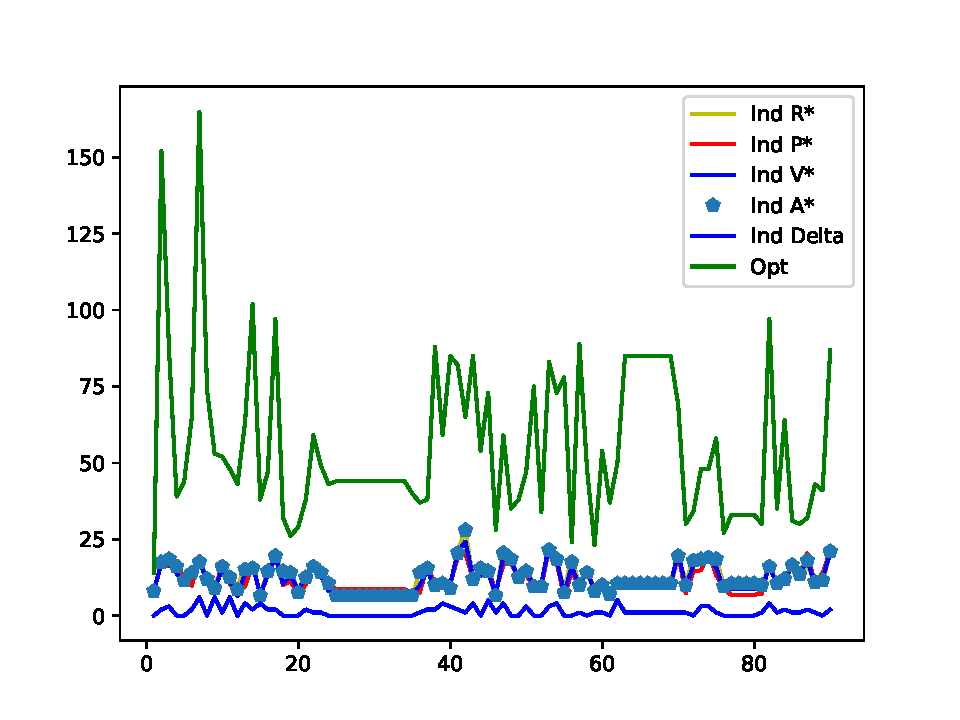
\includegraphics[width=9cm]{images_these/Indicateurs_time_90.pdf}\hfill
%	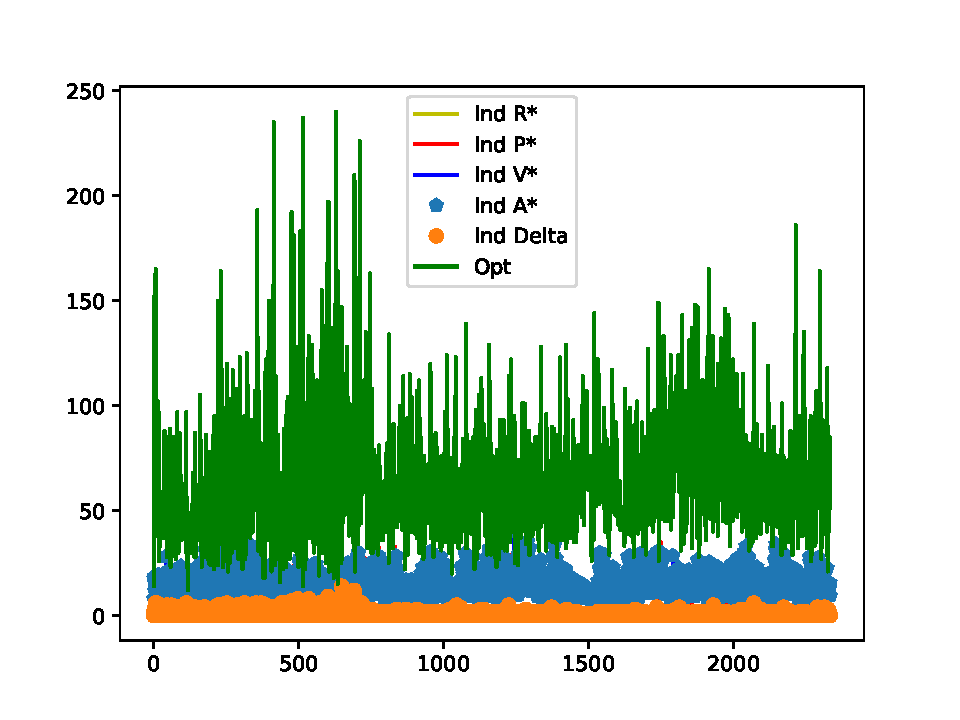
\includegraphics[width=9cm]{images_these/Indicateurs_time.pdf}
%	\caption{Indicateurs de temps sans $G$ }\label{Indicateurs_time}
%\end{figure}
%
%\begin{figure}
%	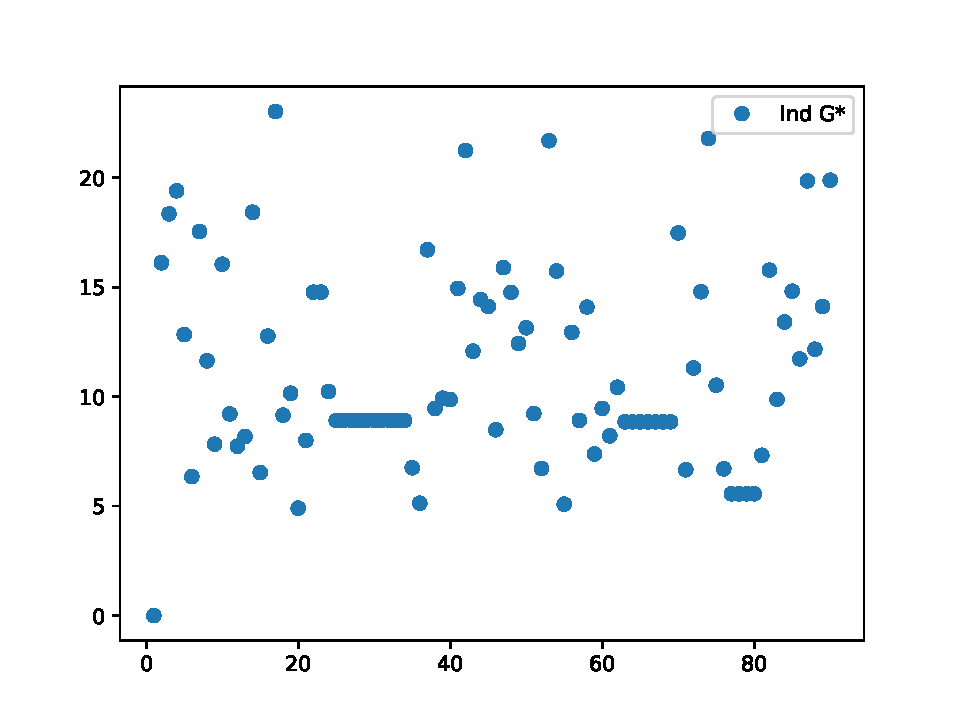
\includegraphics[width=9cm]{images_these/Indicateurs_time_G_90.pdf}\hfill
%	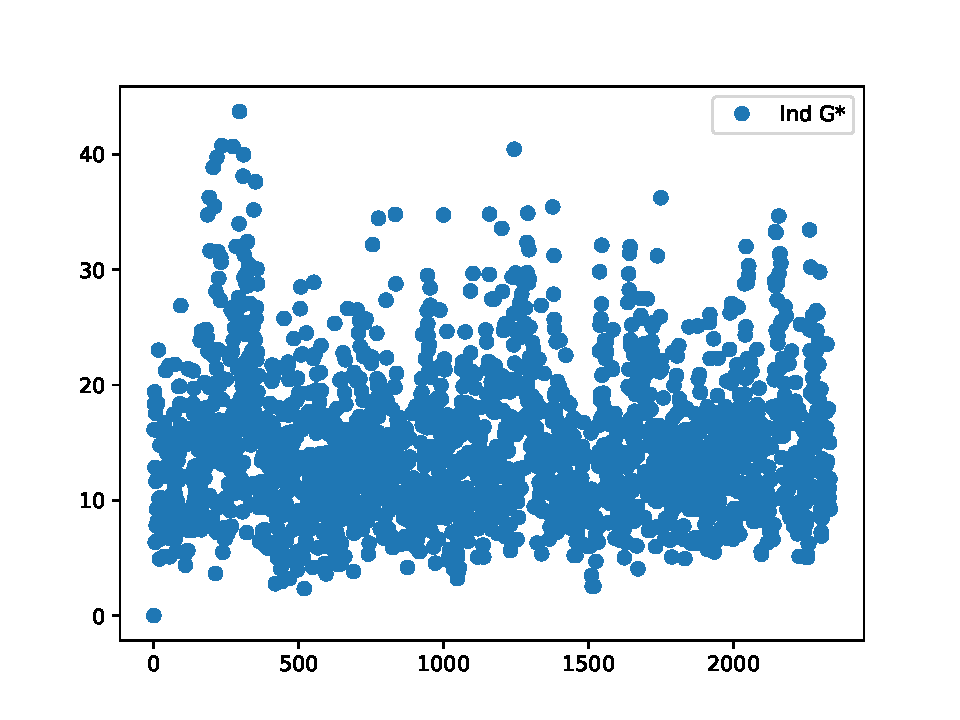
\includegraphics[width=9cm]{images_these/Indicateurs_time_G.pdf}
%	\caption{Indicateurs de temps G}\label{Indicateurs_time_G}
%\end{figure}
%
%\begin{figure}
%	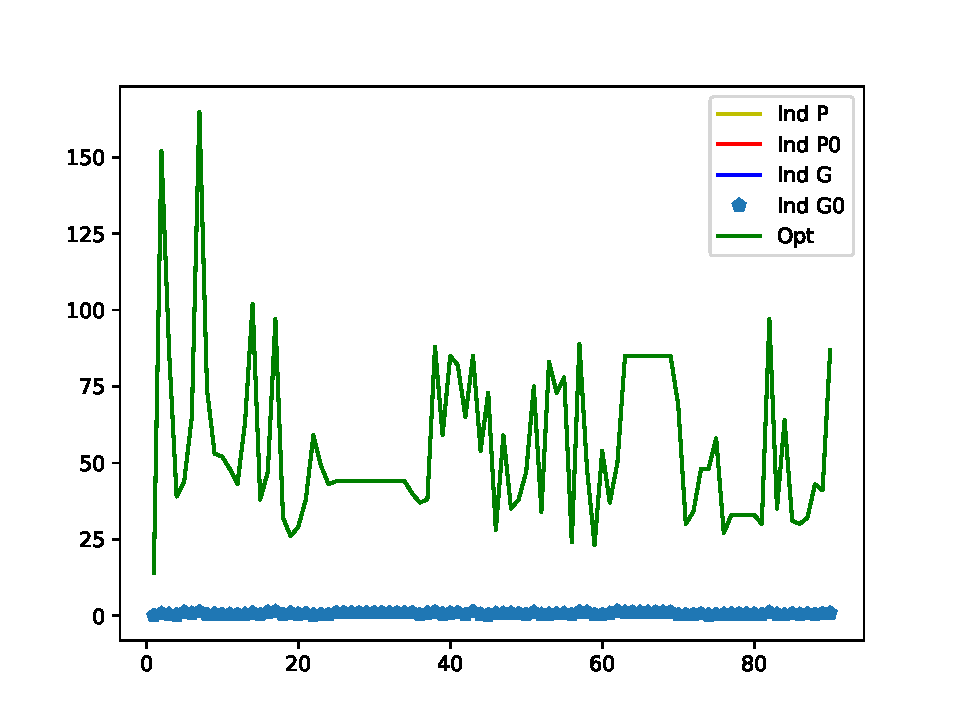
\includegraphics[width=9cm]{images_these/Indicateurs_unit_90.pdf}\hfill
%	\includegraphics[width=9cm]{images_these/Indicateurs_unit.pdf}
%	\caption{Indicateurs de coût unitaire}\label{Indicateurs_unit}
%\end{figure}
%
%\begin{figure}
%	\includegraphics[width=9cm]{images_these/Indicateurs_absolute_90.pdf}\hfill
%	\includegraphics[width=9cm]{images_these/Indicateurs_absolute.pdf}
%	\caption{Indicateurs de coût absolu}\label{Indicateurs_absolute}
%\end{figure}
\subsection{Moyenne de la valeur absolue des gaps} 

Le but de cette section est de présenter les gaps obtenus après entrainement de nos réseaux de neurones. La métrique d'évaluation de nos réseaux est le gap entre la valeur $V_{Opt}$ utilisée pour entrainer nos réseaux et la valeur $V_{Predit}$ prédit par nos réseaux : $(|V_{Opt}-V_{Predit}|/V_{Opt})$. On présente ici la moyenne des gaps des données d'apprentissage et des données de test.
On trouve au tableau (\ref{Gap}) les résultats de nos réseaux qui prédisent le coût de production. On trouve au tableau (\ref{Gap_time}) les résultats de nos réseaux qui prédisent le numéro de période de la dernière recharge. La signification de chaque colonne est :
\begin{itemize}[label=$\square$]
	\item La colonne nommée \og Nom du réseau de neurones \fg{} est le nom du réseau de neurones ;
	\item La colonne nommée \og fig. réseau \fg{} donne les numéros des figures qui illustrent l'architecture du réseau de neurones ;
	\item La colonne nommée \og fig. résultats \fg{} donne le numéro de figures qui illustrent la courbe des valeurs prédites par le réseau de neurones, la courbe des valeurs utilisées pour entrainer le réseau de neurones et les courbes de l'évolution du gap au fil des itérations ;
	\item La colonne nommée \og \# itérations \fg{} est le nombre d'itérations ;
	\item La colonne nommée \og  Gap test\fg{} est la moyenne en pourcentage des gaps des données de test ;
	\item La colonne nommée \og Gap entrainement \fg{} est la moyenne en pourcentage des gaps des données d'entrainement ;
	\item La colonne nommée \og \# poids \fg{} est le nombre de poids synaptiques des réseaux de neurones.
\end{itemize}
%la moyenne de la valeur absolue des gaps des données de test et le nombre de poids et biais correspondant à chaque algorithme.

\begin{table}[H]
	\begin{center}
	\begin{tabular}{|m{4.5cm}|m{2cm}|m{2.5cm}|m{1.9cm}|m{1.5cm}|m{1.5cm}|m{1.5cm}|}
	\hline
%	\rowcolor{cyan}Nom du réseau de neurones (Partie production)(2620 instances) &fig. réseau&fig. résultats&\# itérations& Gap (\%)& \# poids\\
%	\hline
%	Perceptron Multicouche (Données classées par période)& (\ref{SFC})& (\ref{loss_sequentialModel_by_period_1}) (\ref{SequentialModel_prediction_by_period_1})& 200&17,85& 2 649\\
%	\hline
%	Perceptron Multicouche (Données classées par type) & (\ref{SFC})& (\ref{loss_sequentialModel_by_type_0}) (\ref{SequentialModel_prediction_by_type_0}) &200&19,57&2 617 \\
%	\hline
%	Réseau fonctionnel initial&  (\ref{FNFC})& (\ref{loss_prediction_courbe_Al_He_}) (\ref{prediction_courbe_Al_He_complet}) &200&16,91 & 38 800 \\
%	\hline
%%	Réseau fonctionnel avec dropout 0,5& (\ref{FNFC})& (\ref{Drop_loss_prediction_courbe_Al_He_}) (\ref{Drop_prediction_courbe_Al_He_complet})&200&   & 22 720\\
%%	\hline
%%	Réseau fonctionnel avec dropout 0,8& (\ref{FNFC})& (\ref{Drop2_loss_prediction_courbe_Al_He_}) (\ref{Drop2_prediction_courbe_Al_He_complet})&200&   & \\
%%	\hline
%	Réseau fonctionnel avec compactation $N\leq20$& (\ref{FNFC})& (\ref{N20_PROD_loss_prediction_reseauALternativeLearning}) (\ref{N20_PROD_prediction_reseauALternativeLearning})&200&  14,19 & 2500\\
%	\hline
%%	Réseau fonctionnel avec compactation $N\leq20$&  (\ref{FNFC})& (\ref{N20_PROD_2000_loss_prediction_reseauALternativeLearning}) (\ref{N20_PROD_2000_prediction_reseauALternativeLearning})&2000&  17,9 & 2500\\
%%	\hline
%	Réseau basé sur les indicateurs&(\ref{1_PROD_cost_value})(\ref{2_PROD_cost_value}) (\ref{PROD_cost_value})&(\ref{PROD_loss_prediction_reseauALternativeLearning})  (\ref{PROD_prediction_reseauALternativeLearning}) &200& 19,53& 14 \\
%	\hline
	\rowcolor{cyan}Nom du réseau de neurones &fig. réseau&fig. résultats &\# itérations& Gap test(\%)&Gap entrainement(\%)& \# poids\\
	\hline
	Réseau \textbf{SIMPLE\_TYPE} & (\ref{SFC})& (\ref{6000_loss_sequentialModel_by_type_0}) (\ref{6000_SequentialModel_prediction_by_type_0}) &20&25,45&24,8 &697\\
	\hline
	Réseau \textbf{SIMPLE\_PERIODE}& (\ref{SFC2})& (\ref{6000_loss_sequentialModel_by_period_1}) (\ref{6000_SequentialModel_prediction_by_period_1})& 2&23,28 &38,03 & 729\\
	\hline
	Réseau \textbf{MIXTE\_COUT}&  (\ref{FNFC})& (\ref{6000_loss_prediction_courbe_Al_He_}) (\ref{6000_prediction_courbe_Al_He_complet}) &161&17,14 & 14,49&570\\
	\hline
	Réseau \textbf{INDIC\_COUT}&(\ref{1_PROD_cost_value})(\ref{2_PROD_cost_value}) (\ref{PROD_cost_value})&(\ref{6000_PROD_loss_prediction_reseauALternativeLearning})  (\ref{6000_PROD_prediction_reseauALternativeLearning}) &201&24,19 &13,27 & 20\\
	\hline
\end{tabular}
	\end{center}
\caption[Apprentissage du coût de production : Moyenne de la valeur absolue des gaps des données de test et d'apprentissage ]{Apprentissage du coût de production : Moyenne de la valeur absolue des gaps des données de test et d'apprentissage. \label{Gap}}
\end{table}

\begin{table}[H]
	\begin{center}
		\begin{tabular}{|m{4cm}|m{2cm}|m{2.5cm}|m{1.9cm}|m{1.5cm}|m{2cm}|m{1.5cm}|}
%			\hline
%			\rowcolor{cyan}Nom du réseau de neurones (Partie recharge) (2620 instances) &fig. réseau & fig. résultats&\# itérations& Gap (\%)& \# poids\\
%			\hline
%			Réseau fonctionnel initial&  (\ref{FNFC})& (\ref{time_loss_prediction_courbe_Al_He_}) (\ref{time_prediction_courbe_Al_He_complet}) &200&18,59 & 38 800\\
%			\hline
%%			Réseau fonctionnel avec dropout 0,5& (\ref{FNFC})& (\ref{Drop_loss_prediction_courbe_Al_He_}) (\ref{Drop_prediction_courbe_Al_He_complet})&200&   & 22 720\\
%%			\hline
%%			Réseau fonctionnel avec dropout 0,8& (\ref{FNFC})& (\ref{Drop2_loss_prediction_courbe_Al_He_}) (\ref{Drop2_prediction_courbe_Al_He_complet})&200&   & \\
%%			\hline
%			Réseau fonctionnel avec compactation $N\leq20$& (\ref{FNFC})& (\ref{time_N20_PROD_loss_prediction_reseauALternativeLearning}) (\ref{time_N20_PROD_prediction_reseauALternativeLearning})&200&  16,44  & 2500\\
%			\hline
%			Réseau basé sur les indicateurs&(\ref{time_value_scheme})&(\ref{loss_prediction_reseauALternativeLearning}) (\ref{prediction_reseauALternativeLearning}) &200& 11,28& 9 \\
			\hline
				\rowcolor{cyan}Nom du réseau de neurones &fig. réseau & fig. résultats&\# itérations& Gap test (\%)&Gap entrainement(\%)& \# poids\\
			\hline
			Réseau \textbf{MIXTE\_TEMPS}&  (\ref{FNFC})& (\ref{time_6000_loss_prediction_courbe_Al_He_}) (\ref{time_6000_prediction_courbe_Al_He_complet}) &195&11,26 & 8,31& 570 \\
			\hline
			Réseau \textbf{INDIC\_TEMPS}&(\ref{time_value_scheme})&(\ref{6000_loss_prediction_reseauALternativeLearning}) (\ref{6000_prediction_reseauALternativeLearning}) &3& 13,21 &8,78 &9 \\
			\hline
		\end{tabular}
	\end{center}
	\caption[Apprentissage du numéro de période de la dernière recharge : Moyenne de la valeur absolue des gaps des données de test et d'apprentissage ]{Apprentissage du numéro de période de la dernière recharge : Moyenne de la valeur absolue des gaps des données de test et d'apprentissage. \label{Gap_time}}
\end{table}

Notre objectif en terme de gap lorsqu'on construisait nos réseaux de neurones était d'être en dessous de 5\%, ce qui est la plupart du temps le cas d'une bonne heuristique en recherche opérationnelle. Autrement dit, on espérait ne pas être très loin des résultats d'une heuristique mais ce n'est malheureusement pas le cas.
Les gaps des réseaux \textbf{SIMPLE\_TYPE} et \textbf{SIMPLE\_PERIODE} sont les plus élevés, peut-être est-ce à cause de la \og simplicité \fg{} de ces réseaux. 
On est assez déçu des résultats des réseaux \textbf{MIXTE\_COUT} et \textbf{MIXTE\_TEMPS}. %car ceux sont les réseaux qui ont le plus grand nombre de poids, on s'attendait à un meilleur gap.
Les gaps du réseau \textbf{INDIC\_COUT} ne sont pas très décevants au vu du faible nombre de poids de ce réseau. Cela est peut-être dû au fait qu'on a peu d'indicateurs. %On constate ici que le gap du réseau \textbf{INDIC\_COUT} des données d'entrainement est supérieur à celui des données de test peut-être est-ce dû au fait qu'on a juste 90 instances de test contre 5910 instances d'apprentissage. 
%On constate que le réseau \textbf{MIXTE\_TEMPS} donne un grand écart entre le gap des données d'apprentissage et le gap des données de test. 

La capacité de généralisation d'un réseau est sa capacité à faire de bonnes prédictions sur de nouvelles données. La capacité de généralisation se mesure ici à l'aide des gaps des données de test. On constate ici que les réseaux qui ont la meilleure capacité de généralisation sont les réseaux \textbf{MIXTE\_COUT} et \textbf{MIXTE\_TEMPS}. Tandis que les réseaux qui ont un gap d'entrainement le plus faible sont les réseaux \textbf{INDIC\_COUT} et \textbf{MIXTE\_TEMPS}.


\subsection{Résultats des réseaux \textbf{SIMPLE\_TYPE} et  \textbf{SIMPLE\_PERIODE}}
La fonction d'activation permet de changer la façon dont une valeur est représentée. Nous allons tester plusieurs fonctions d'activation sur le réseau \textbf{SIMPLE\_PERIODE}.
La liste de fonctions qu'on testera est la suivante :
\begin{itemize}[label=$\square$]
	\item La fonction linéaire :
	$f(x)=x$, elle laisse passer toutes les valeurs dans les couches suivantes. 
	\item La fonction relu (Rectified Linear Unit) :
	$$
	f(x)= \left\{
	\begin{array}{ll}
	0 & \mbox{si x<0} \\
	x & \mbox{si x $\geq$ 0.}
	\end{array}
	\right.
	$$
Elle ne laisse passer dans les couches suivantes que les valeurs positives. 
\item La fonction elu (Exponential Linear Unit) : 
$$
f(x)= \left\{
\begin{array}{ll}
\alpha \times (e^x - 1) & \mbox{si x<0} \\
x & \mbox{si x $\geq$ 0.}
\end{array}
\right.
$$
Elle est une amélioration de la fonction RELU car elle lisse aussi les valeurs négatives
\item La fonction  selu (Scaled Exponential Linear Unit) est une amélioration de la fonction elu.

$$
f(x)= \left\{
\begin{array}{ll}
scale \times \alpha \times (e^x - 1) & \mbox{si x<0} \\
scale \times x & \mbox{si x $\geq$ 0.}
\end{array}
\right.
$$
Les valeurs utilisées sont les valeurs par défaut $\alpha = 1,67326324$, $scale = 1,05070098$.
\item La fonction softplus : $f(x)=log(e^x + 1)$, est une approximation de la fonction relu.
	\item La fonction sigmoïde : 
${\displaystyle f(x)={\frac {1}{1+{\rm {e}}^{-x}}}}$ elle donne une valeur dans l'intervalle [0,1].
	
\item La fonction tangente hyperbolique ${\displaystyle f(x)={\frac {1-{\rm {e}}^{-2x}}{1+{\rm {e}}^{-2x}}}}$  elle donne une valeur dans l'intervalle [-1,1].
		
	\end{itemize}

Le tableau (\ref{comp_act}) présentent les gaps obtenus avec le réseau \textbf{SIMPLE\_PERIODE} lorsqu'on modifie les fonctions d'activation de la couche d'entrées et de la couche cachée. La signification des colonnes est :
\begin{itemize}[label=$\square$]
	\item La colonne \og Activation couche 1 \fg{} donne le nom de la fonction d'activation utilisée pour la couche d'entrées du réseau \textbf{SIMPLE\_PERIODE}
	\item La colonne \og Activation couche 2 \fg{} donne le nom de la fonction d'activation utilisée pour la couche cachée du réseau \textbf{SIMPLE\_PERIODE}
	\item La colonne nommée \og  Gap test\fg{} est la moyenne en pourcentage des gaps des données de test ;
	\item La colonne nommée \og Gap entrainement \fg{} est la moyenne en pourcentage des gaps des données d'entrainement ;
	
\end{itemize}

On constate que le fait de changer la façon dont les données d'entrées sont classées a une influence sur les résultats de nos réseaux. De plus, on constate aussi que le fait de changer de fonction d'activation a une influence sur les résultats de nos réseaux.
 On constate que c'est la fonction selu qui nous donne le meilleur gap sur les données de test. C'est donc cette fonction que nous utiliserons pour tester les réseaux \textbf{SIMPLE\_TYPE} et \textbf{SIMPLE\_PERIODE}.

\begin{table}[H]
	\begin{center}
		\begin{tabular}{|m{4cm}|m{4cm}|m{3cm}|m{4cm}|}
\hline
\rowcolor{cyan} Activation couche 1 &Activation couche 2 & Gap entrainement(\%)&Gap test (\%)\\
\hline
linéaire&linéaire &89,08&188,34\\\hline
tangente h.&tangente h.&67,10&41,88\\\hline
sigmoide&sigmoide&66,68 & 40,99\\\hline
relu&relu&21,52&33,47\\\hline
relu&selu&21,54&28,75\\\hline
selu&relu&17,69&27,86\\\hline
softplus&softplus&20,03&21,63\\\hline
elu&elu&19,95&21,67 \\\hline
selu&selu&20&21,14\\\hline

\end{tabular}
\end{center}
\caption[Comparaison des fonctions d'activation du réseau SIMPLE\_PERIODE]{Comparaison des fonctions d'activation du réseau \textbf{SIMPLE\_PERIODE}. \label{comp_act} }
\end{table}
 %\begin{figure}[H]
%	\centerline{
%		\includegraphics[height=7cm]{images_these/SFC_by_period_1.pdf}}
%	\caption[Modèle séquentiel complètement connecté (période)]{Modèle séquentiel complètement connecté avec les données classées par période.}
%	\label{SFC_by_period_1}
%\end{figure}

%\begin{figure}[H]
%	\centerline{
%		\includegraphics[height=7cm]{images_these/SFC_by_type_0.png}}
%	\caption[Modèle séquentiel complètement connecté (type)]{Modèle séquentiel complètement connecté avec les données classées par type.}
%	\label{SFC_by_type_0}
%\end{figure}



\subsubsection{Résultats du réseau \textbf{SIMPLE\_TYPE}}
%On a 2617 poids et biais.

La figure (\ref{6000_loss_sequentialModel_by_type_0}) représente l'évolution du gap moyen des données d'apprentissage (courbe bleue) et des données de test (courbe rouge) lorsqu'on augmente le nombre d'itérations. L'axe des abscisses est le nombre d'itérations et l'axe des ordonnées est le gap moyen. Par souci de lisibilité, on a limité l'axe des ordonnées à l'intervalle [0,200] car on veut pouvoir clairement voir l'écart entre les deux courbes. Globalement, ce gap décroit. On constate que le gap ici se stabilise vite. Au bout d'environ 25 itérations, on a déjà un gap assez stable, mais après 100 itérations les gaps redeviennent un peu instables. Le nombre d'itérations maximal correspond à l'itération qui a fournit le plus petit gap sur les données de test.

 Les résultats du réseau \textbf{SIMPLE\_TYPE} sont illustrés par les figures  (\ref{6000_SequentialModel_prediction_by_type_0}). On veut voir la corrélation entre les valeurs prédites par le réseau et les valeurs optimales utilisées pour entrainer le réseau. L'axe des abscisses est respectivement pour la figure (\ref{6000_SequentialModel_prediction_by_type_0}) (a) et (\ref{6000_SequentialModel_prediction_by_type_0}) (b) les instances d'apprentissage triées par coût de production croissant et regroupées par paquet de 100 et les instances de test triées par coût de production croissant. L'axe des ordonnées est respectivement pour la figure (\ref{6000_SequentialModel_prediction_by_type_0}) (a) et (\ref{6000_SequentialModel_prediction_by_type_0}) (b) le coût de production moyen et le coût de production. La courbe verte est la courbe des valeurs optimales et la courbe rouge est la courbe des valeurs prédites par le réseau de la figure (\ref{SFC}). (a) représente les données d'apprentissage et (b) représente les données de test. En observant la courbe (a), on a l'impression que le réseau fait de bonnes prédictions mais c'est trompeur car on a fait des paquets de 100 instances et on a fait des moyennes sur ces paquets, ce qui a pour conséquence de compenser les erreurs. Le fait de faire des moyennes a lissé la courbe des valeurs prédites de la figure (\ref{6000_SequentialModel_prediction_by_type_0}) (a) sinon cette dernière se présente aussi en dents de scie. On observe que la courbe des valeurs prédites a l'allure de la courbe des valeurs optimales avec une tendance à être légère en dessous de celle-ci après environ l'itération 45 et à être au dessus avant cette itération.
 
 
On constate que le réseau \textbf{SIMPLE\_TYPE} est de mauvaise qualité, ceci peut s'expliquer par le fait que ce réseau est \og simple \fg{}, c'est-à-dire qu'il n'épouse pas la logique de notre problème.

%\begin{figure}[H]
%	\centerline{
%		\includegraphics[height=7cm]{images_these/loss_sequentialModel_by_type_0.pdf}}
%	\caption[La fonction de perte (\textit{Loss}) du réseau séquentiel complètement connecté (type)]{La fonction de perte (\textit{Loss}) du réseau séquentiel complètement connecté avec les données classées par type.}
%	\label{loss_sequentialModel_by_type_0}
%\end{figure}
%
%
%\begin{figure}
%	(a)\includegraphics[width=9cm]{images_these/SequentialModel_prediction_test_by_type_0.pdf}\hfill
%	(b)\includegraphics[width=9cm]{images_these/SequentialModel_prediction_train_by_type_0.pdf}
%	\caption{Résultats du réseau de neurones séquentiel pour la prédiction du coût de production avec des données classées type par type. (a) représente les données de test et (b) représente les données d'apprentissage.}\label{SequentialModel_prediction_by_type_0}
%\end{figure}

\begin{figure}[H]
	\centerline{
		\includegraphics[height=7cm]{images_these/Gap_PROD_prediction_sequentialModel_test_valid_data__by_type.pdf}}
	\caption[Le gap du réseau SIMPLE\_TYPE]{Cette figure représente l'évolution du gap lorsqu'on fait varier le nombre d'itérations lors de l'apprentissage du réseau \textbf{SIMPLE\_TYPE}. Ici, les données d'entrées sont classées par type. La courbe bleue est l'évolution de l'erreur sur les données d'apprentissage et la courbe rouge est l'évolution de l'erreur sur les données de test. Le nombre d'itérations maximal correspond à l'itération qui a fournit le plus petit gap sur les données de test.}
	\label{6000_loss_sequentialModel_by_type_0}
\end{figure}


%\begin{figure}
%	(a)\includegraphics[width=9cm]{images_these/6000_SequentialModel_prediction_test_by_type_0.pdf}\hfill
%	(b)\includegraphics[width=9cm]{images_these/6000_SequentialModel_prediction_train_by_type_0.pdf}
%	\caption{Résultats du réseau de neurones séquentiel pour la prédiction du coût de production avec des données classées type par type. (a) représente les données de test et (b) représente les données d'apprentissage.}\label{6000_SequentialModel_prediction_by_type_0}
%\end{figure}

\begin{figure}[H]
	\centering
	\begin{tabular}{c c}
		\includegraphics[width=9cm]{images_these/SequentialModel_prediction_train_by_type.pdf}&
		\includegraphics[width=9cm]{images_these/SequentialModel_prediction_test_by_type.pdf}
		\\
		(a) & (b)
	\end{tabular}
	\caption[Résultats du réseau de neurones SIMPLE\_TYPE]{Résultats du réseau de neurones \textbf{SIMPLE\_TYPE} pour la prédiction du coût de production avec des données classées type par type. (a) représente les données d'apprentissage et (b) représente les données de test. La courbe rouge est la courbe des valeurs prédites et la courbe verte est la courbe des valeurs optimales.}\label{6000_SequentialModel_prediction_by_type_0}
\end{figure}
  
  
  \subsubsection{Résultats du réseau \textbf{SIMPLE\_PERIODE}}
  
  % (\ref{loss_sequentialModel_by_period_1}), (\ref{SequentialModel_prediction_by_period_1}),
  
  La figure (\ref{6000_loss_sequentialModel_by_period_1}) représente l'évolution du gap moyen des données d'apprentissage (courbe bleue) et des données de test (courbe rouge) lorsqu'on augmente le nombre d'itérations. L'axe des abscisses est le nombre d'itérations et l'axe des ordonnées est le gap moyen. Par souci de lisibilité, on a limité l'axe des ordonnées à l'intervalle [0,200] car on veut pouvoir clairement voir l'écart entre les deux courbes. Globalement, ce gap décroit. On constate que le gap sur les données d'apprentissage se stabilise vite, au bout d'environ 10 itérations, on a déjà un gap assez stable. Tandis que le gap sur les données de test se stabilise au bout d'environ 185 itérations. Le nombre d'itérations maximal correspond à l'itération qui a fournit le plus petit gap sur les données de test.
  
  Les résultats du réseau \textbf{SIMPLE\_PERIODE} sont illustrés par les figures  (\ref{6000_SequentialModel_prediction_by_period_1}). On veut voir la corrélation entre les valeurs prédites par le réseau et les valeurs optimales utilisées pour entrainer le réseau. L'axe des abscisses représente respectivement pour la figure (\ref{6000_SequentialModel_prediction_by_period_1}) (a) et (\ref{6000_SequentialModel_prediction_by_period_1}) (b) les instances d'apprentissage  triées par coût de production croissant et regroupées par paquet de 100 et les instances de test triées par coût de production croissant. L'axe des ordonnées est respectivement pour la figure (\ref{6000_SequentialModel_prediction_by_period_1}) (a) et (\ref{6000_SequentialModel_prediction_by_period_1}) (b) le coût de production moyen et le coût de production. La courbe verte est la courbe des valeurs optimales et la courbe rouge est la courbe des valeurs prédites par le réseau de la figure (\ref{SFC2}). La figure (a) représente les données d'apprentissage et la figure (b) représente les données de test. En observant les courbes (a), on a l'impression que le réseau fait de bonnes prédictions mais c'est trompeur car on a fait des paquets de 100 instances et on a fait des moyennes sur ces paquets, ce qui a pour conséquence de compenser les erreurs. Le fait de faire des moyennes a lissé la courbe des valeurs prédites de la figure (\ref{6000_SequentialModel_prediction_by_period_1}) (a) sinon cette dernière se présente aussi en dents de scie. On observe que la courbe des valeurs prédites a l'allure de la courbe des valeurs optimales avec une tendance à être légère en dessous de celle-ci après environ l'itération 43 et à être au dessus avant cette itération.
  
%Les résultats du réseau \textbf{SIMPLE\_PERIODE} se trouvent aux figures (\ref{6000_SequentialModel_prediction_by_period_1}). 
  On constate que le réseau \textbf{SIMPLE\_PERIODE} est de mauvaise qualité, ceci s'explique par le fait que ce réseau est \og simple\fg{}, c'est-à-dire qu'il n'épouse pas la logique de notre problème.
  
  
  %\begin{figure}[!ht]
  %	\centerline{
  %		\includegraphics[height=7cm]{images_these/loss_sequentialModel_by_period_1.pdf}}
  %	\caption[La fonction de perte (\textit{Loss}) du réseau séquentiel complètement connecté (période)]{La fonction de perte (\textit{Loss}) du réseau séquentiel complètement connecté avec les données classées par période.}
  %	\label{loss_sequentialModel_by_period_1}
  %\end{figure}
  %
  %
  %\begin{figure}
  %	(a)\includegraphics[width=9cm]{images_these/SequentialModel_prediction_test_by_period_1.pdf}\hfill
  %		(b)\includegraphics[width=9cm]{images_these/SequentialModel_prediction_train_by_period_1.pdf}
  %	\caption{Résultats du réseau de neurones séquentiel pour la prédiction du coût de production avec des données classées par période. (a) représente les données de test et (b) représente les données d'apprentissage.}\label{SequentialModel_prediction_by_period_1}
  %\end{figure}
  
  \begin{figure}[H]
  	\centerline{
  		\includegraphics[height=7cm]{images_these/Gap_PROD_prediction_sequentialModel_test_valid_data__by_period.pdf}}
  	\caption[Le gap du réseau SIMPLE\_PERIODE]{Cette figure représente l'évolution du gap lorsqu'on fait varier le nombre d'itérations lors de l'apprentissage du réseau \textbf{SIMPLE\_PERIODE}. Ici, les données d'entrées sont classées par période. La courbe bleue est l'évolution de l'erreur sur les données d'apprentissage et la courbe rouge est l'évolution de l'erreur sur les données de test. Le nombre d'itérations maximal correspond à l'itération qui a fournit le plus petit gap sur les données de test.}
  	\label{6000_loss_sequentialModel_by_period_1}
  \end{figure}
  
  
  %\begin{figure}
  %	(a)\includegraphics[width=9cm]{images_these/6000_SequentialModel_prediction_test_by_period_1.pdf}\hfill
  %	(b)\includegraphics[width=9cm]{images_these/6000_SequentialModel_prediction_train_by_period_1.pdf}
  %	\caption{Résultats du réseau de neurones séquentiel pour la prédiction du coût de production avec des données classées par période. (a) représente les données de test et (b) représente les données d'apprentissage.}\label{6000_SequentialModel_prediction_by_period_1}
  %\end{figure}
  
  \begin{figure}[H]
  	\centering
  	\begin{tabular}{c c}
  		\includegraphics[width=9cm]{images_these/SequentialModel_prediction_train_by_period.pdf}&
  		\includegraphics[width=9cm]{images_these/SequentialModel_prediction_test_by_period.pdf} 
  		\\
  		(a) & (b)
  	\end{tabular}
  	\caption[Résultats du réseau SIMPLE\_PERIODE]{Résultats du réseau \textbf{SIMPLE\_PERIODE} pour la prédiction du coût de production avec des données classées par période. (a) représente les données d'apprentissage et (b) représente les données de test . La courbe rouge est la courbe des valeurs prédites et la courbe verte est la courbe des valeurs optimales.}\label{6000_SequentialModel_prediction_by_period_1}
  \end{figure}
  
%\subsection{Résultats du modèle fonctionnel complètement connecté}

%\begin{figure}[!ht]
%	\centerline{
%		\includegraphics[height=7cm]{images_these/reseauFunctional_by_period_1.pdf}}
%	\caption[Modèle fonctionnel complètement connecté (période)]{Modèle fonctionnel complètement connecté avec des données classées par période.}
%	\label{reseauFunctional_by_period_0}
%\end{figure}


%\begin{figure}[!ht]
%	\centerline{
%		\includegraphics[height=7cm]{images_these/reseauFunctional_by_type_0.pdf}}
%	\caption[Modèle fonctionnel complètement connecté (type)]{Modèle fonctionnel complètement connecté avec des données classées par type.}
%	\label{reseauFunctional_by_type_0}
%\end{figure}


%\subsubsection{Résultats pour les données d'entrées classées par période}
%On a 3049 poids et biais

%Voir figure (\ref{loss_functionalModel_by_period_0}), (\ref{functionalModel_prediction_by_period_0})



%\begin{figure}[!ht]
%	\centerline{
%		\includegraphics[height=7cm]{images_these/loss_functionalModel_by_period_1.pdf}}
%	\caption[Perte du modèle fonctionnel complètement connecté (période)]{Perte du modèle fonctionnel complètement connecté avec les données classées par période.}
%	\label{loss_functionalModel_by_period_0}
%\end{figure}


%\begin{figure}
%	\includegraphics[width=9cm]{images_these/functionalModel_prediction_test_by_period_1.pdf}\hfill
%	\includegraphics[width=9cm]{images_these/functionalModel_prediction_train_by_period_1.pdf}
%	\caption{réseau de neurones fonctionnel pour la prédiction du coût de production avec des données classées par type}\label{functionalModel_prediction_by_period_0}
%\end{figure}


%\subsubsection{Résultats pour les données d'entrées classées par type}
%On a 3013 poids et biais

%Voir figure (\ref{loss_functionalModel_by_type_0}), (\ref{functionalModel_prediction_by_type_0})


%\begin{figure}[!ht]
%	\centerline{
%		\includegraphics[height=7cm]{images_these/loss_functionalModel_by_type_0.pdf}}
%	\caption[Perte du modèle fonctionnel complètement connecté (type)]{Perte du modèle fonctionnel complètement connecté avec les données classées par type.}
%	\label{loss_functionalModel_by_type_0}
%\end{figure}


%\begin{figure}
%	\includegraphics[width=9cm]{images_these/functionalModel_prediction_test_by_type_0.pdf}\hfill
%	\includegraphics[width=9cm]{images_these/functionalModel_prediction_train_by_type_0.pdf}
%	\caption{réseau de neurones fonctionnel pour la prédiction du coût de production avec des données classées type par type}\label{functionalModel_prediction_by_type_0}
%\end{figure}


\subsection{Résultats du réseau \textbf{MIXTE\_COUT} pour la prédiction du coût de production}

La figure (\ref{6000_loss_prediction_courbe_Al_He_}) représente l'évolution du gap moyen des données d'apprentissage (courbe bleue) et des données de test (courbe rouge) lorsqu'on augmente le nombre d'itérations. L'axe des abscisses est le nombre d'itérations et l'axe des ordonnées est le gap moyen. Par souci de lisibilité, on a limité l'axe des ordonnées à l'intervalle [0,50] car on veut pouvoir clairement voir l'écart entre les deux courbes. Globalement, ce gap décroit. On constate que le gap ici se stabilise vite. Au bout d'environ 50 itérations, on a déjà un gap assez stable. Le nombre d'itérations maximal correspond à l'itération qui a fournit le plus petit gap sur les données de test.

Les résultats du réseau \textbf{MIXTE\_COUT} pour la prédiction du coût de production sont illustrés par les figures  (\ref{6000_prediction_courbe_Al_He_complet}). On veut voir la corrélation entre les valeurs prédites par le réseau et les valeurs optimales  utilisées pour entrainer le réseau. L'axe des abscisses est respectivement pour la figure (\ref{6000_prediction_courbe_Al_He_complet}) (a) et (\ref{6000_prediction_courbe_Al_He_complet}) (b) les instances d'apprentissage triées par coût de production croissant et regroupées par paquet de 100 et les instances de test triées par coût de production croissant. L'axe des ordonnées est respectivement pour la figure (\ref{6000_prediction_courbe_Al_He_complet}) (a) et (\ref{6000_prediction_courbe_Al_He_complet}) (b) le coût de production moyen et le coût de production. La courbe verte est la courbe des valeurs optimales et la courbe rouge est la courbe des valeurs prédites par le réseau de la figure (\ref{FNFC}). La figure (a) représente les données d'apprentissage et la figure (b) représente les données de test. En observant les courbes (a), on a l'impression que le réseau fait de bonnes prédictions mais c'est trompeur car on a fait des paquets de 100 instances et on a fait des moyennes sur ces paquets, ce qui a pour conséquence de compenser les erreurs. Le fait de faire des moyennes a lissé la courbe des valeurs prédites de la figure (\ref{6000_prediction_courbe_Al_He_complet}) (a) sinon cette dernière se présente aussi en dents de scie. On observe que la courbe des valeurs prédites a l'allure de la courbe des valeurs optimales avec une tendance à être au dessus de cette dernière.


%Les résultats du réseau \textbf{MIXTE\_COUT} pour la prédiction du coût de production se trouvent aux figures 
%(\ref{loss_prediction_courbe_Al_He_}), (\ref{prediction_courbe_Al_He_complet}),
  %(\ref{6000_prediction_courbe_Al_He_complet}). 
 %On a 45 441 poids et biais. On obtient ces résultats car le nombre de poids synaptiques est très élevé par rapport aux nombres d'instances d'apprentissage.


%\begin{figure}[!ht]
%	\centerline{
%		\includegraphics[height=7cm]{images_these/loss_prediction_courbe_Al_He_.pdf}}
%	\caption[La fonction de perte (\textit{Loss}) du perceptron multicouche fonctionnel]{La fonction de perte (\textit{Loss}) du perceptron multicouche fonctionnel.}
%	\label{loss_prediction_courbe_Al_He_}
%\end{figure}
%
%
%\begin{figure}
%	(a)\includegraphics[width=9cm]{images_these/prediction_courbe_Al_He_complet_test.pdf}\hfill
%		(b)\includegraphics[width=9cm]{images_these/prediction_courbe_Al_He_complet_train.pdf}
%	\caption{Résultats du réseau de neurones du perceptron multicouche fonctionnel. (a) représente les données de test et (b) représente les données d'apprentissage.}\label{prediction_courbe_Al_He_complet}
%\end{figure}

\begin{figure}[H]
	\centerline{
		\includegraphics[height=7cm]{images_these/Gap_PROD_prediction_reseaufonctionnel_testtrain_data2.pdf}}
	\caption[Le gap du réseau MIXTE\_COUT]{Cette figure représente l'évolution du gap lorsqu'on fait varier le nombre d'itérations lors de l'apprentissage du réseau \textbf{MIXTE\_COUT} pour la prédiction du coût de production. La courbe bleue est l'évolution de l'erreur sur les données d'apprentissage et la courbe rouge est l'évolution de l'erreur sur les données de test. Le nombre d'itérations maximal correspond à l'itération qui a fournit le plus petit gap sur les données de test.}
	\label{6000_loss_prediction_courbe_Al_He_}
\end{figure}


%\begin{figure}
%	(a)\includegraphics[width=9cm]{images_these/6000_prediction_courbe_Al_He_complet_test.pdf}\hfill
%	(b)\includegraphics[width=9cm]{images_these/6000_prediction_courbe_Al_He_complet_train.pdf}
%	\caption{Résultats du réseau de neurones du perceptron multicouche fonctionnel. (a) représente les données de test et (b) représente les données d'apprentissage.}\label{6000_prediction_courbe_Al_He_complet}
%\end{figure}


\begin{figure}[H]
	\centering
	\begin{tabular}{c c}
		\includegraphics[width=9cm]{images_these/prediction_courbe_Al_He_complet_train.pdf}&
		\includegraphics[width=9cm]{images_these/prediction_courbe_Al_He_complet_test.pdf} 
		\\
		(a) & (b)
	\end{tabular}
	\caption[Résultats du  réseau MIXTE\_COUT]{Résultats du  réseau \textbf{MIXTE\_COUT} pour la prédiction du coût de production. (a) représente les données d'apprentissage et (b) représente les données de test. La courbe rouge est la courbe des valeurs prédites et la courbe verte est la courbe des valeurs optimales.}\label{6000_prediction_courbe_Al_He_complet}
\end{figure}

%\subsubsection{Résultats du perceptron multicouche fonctionnel avec \textit{dropout}}
%Si on suppose que les neurones sont désactivés avec la probabilité 0,5 on obtient les résultats des figures
%(\ref{Drop_loss_prediction_courbe_Al_He_}) et (\ref{Drop_prediction_courbe_Al_He_complet}).
%
%\begin{figure}[!ht]
%	\centerline{
%		\includegraphics[height=7cm]{images_these/Drop_loss_prediction_courbe_Al_He_.pdf}}
%	\caption[La fonction de perte (\textit{Loss}) du perceptron multicouche fonctionnel avec \textit{dropout} 0,5]{La fonction de perte (\textit{Loss}) du perceptron multicouche fonctionnel avec \textit{dropout} 0,5.}
%	\label{Drop_loss_prediction_courbe_Al_He_}
%\end{figure}
%
%
%\begin{figure}
%	(a)\includegraphics[width=9cm]{images_these/Drop_prediction_courbe_Al_He_complet_test.pdf}\hfill
%	(b)\includegraphics[width=9cm]{images_these/Drop_prediction_courbe_Al_He_complet_train.pdf}
%	\caption{réseau de neurones du perceptron multicouche fonctionnel avec \textit{dropout} 0,5. (a) représente les données de test et (b) représente les données d'apprentissage.}\label{Drop_prediction_courbe_Al_He_complet}
%\end{figure}
%
%Si on suppose que les neurones sont désactivés avec la probabilité 0,8 on obtient les résultats des figures
%(\ref{Drop2_loss_prediction_courbe_Al_He_}) et (\ref{Drop2_prediction_courbe_Al_He_complet}).
%
%\begin{figure}[!ht]
%	\centerline{
%		\includegraphics[height=7cm]{images_these/Drop2_loss_prediction_courbe_Al_He_.pdf}}
%	\caption[La fonction de perte (\textit{Loss}) du perceptron multicouche fonctionnel avec \textit{dropout} 0,8]{La fonction de perte (\textit{Loss}) du perceptron multicouche fonctionnel avec \textit{dropout} 0,8.}
%	\label{Drop2_loss_prediction_courbe_Al_He_}
%\end{figure}
%
%
%\begin{figure}
%	(a)\includegraphics[width=9cm]{images_these/Drop2_prediction_courbe_Al_He_complet_test.pdf}\hfill
%		(b)\includegraphics[width=9cm]{images_these/Drop2_prediction_courbe_Al_He_complet_train.pdf}
%	\caption{réseau de neurones du perceptron multicouche fonctionnel avec \textit{dropout} 0,8}. (a) représente les données de test et (b) représente les données d'apprentissage.\label{Drop2_prediction_courbe_Al_He_complet}
%\end{figure}
% On constate dans la figure (\ref{Drop2_loss_prediction_courbe_Al_He_}) que la courbe de perte des données d'apprentissage est très proche de celle des données de test. Dans la littérature pour résoudre cela on conseille de soit complexifier le réseau, soit d'ajouter plus de poids, soit de laisser l'entrainement plus longtemps. Du coup, on a laissé l'entrainement plus longtemps en utilisant comme nombre d'itérations 2000 au lieu de 200. On obtient donc les résultats des figures (\ref{Drop2_2000_loss_prediction_courbe_Al_He_}) et (\ref{Drop2_2000_prediction_courbe_Al_He_complet}).
% 
% \begin{figure}[!ht]
% 	\centerline{
% 		\includegraphics[height=7cm]{images_these/Drop2_2000_loss_prediction_courbe_Al_He_.pdf}}
% 	\caption[La fonction de perte (\textit{Loss}) du du perceptron multicouche fonctionnel avec \textit{dropout} 0,8 et epoques=2000]{La fonction de perte (\textit{Loss}) du perceptron multicouche fonctionnel avec \textit{dropout} 0,8 et itérations=2000.}
% 	\label{Drop2_2000_loss_prediction_courbe_Al_He_}
% \end{figure}
% 
% 
% \begin{figure}
% 	\includegraphics[width=9cm]{images_these/Drop2_2000_prediction_courbe_Al_He_complet_test.pdf}\hfill
% 	\includegraphics[width=9cm]{images_these/Drop2_2000_prediction_courbe_Al_He_complet_train.pdf}
% 	\caption{réseau de neurones fonctionnel du perceptron multicouche fonctionnel avec \textit{dropout} 0,8 et itérations =2000}.\label{Drop2_2000_prediction_courbe_Al_He_complet}
% \end{figure}

%\subsubsection{Résultats du réseau \textbf{MIXTE} avec la limitation de N}

%
%Lorsqu'on utilise pour l'apprentissage uniquement des instances dont le nombre de périodes $N\leq40$, on obtient les résultats des figures (\ref{N40_PROD_loss_prediction_reseauALternativeLearning} et (\ref{N40_PROD_prediction_reseauALternativeLearning}). Ici on a 11 521 poids.
%).
%
%\begin{figure}
%	\centerline{
%		\includegraphics[width=9cm]{images_these/N40_PROD_loss_prediction_courbe_Al_He_.pdf}}
%	\caption{La fonction de perte (\textit{Loss})du perceptron multicouche fonctionnel avec $N\leq40$}\label{N40_PROD_loss_prediction_reseauALternativeLearning}
%\end{figure}
%
%
%\begin{figure}
%	\includegraphics[width=9cm]{images_these/N40_PROD_prediction_courbe_Al_He_complet_test.pdf}\hfill
%	\includegraphics[width=9cm]{images_these/N40_PROD_prediction_courbe_Al_He_complet_train.pdf}
%	\caption{réseau de neurones du perceptron multicouche fonctionnel avec $N\leq40$}\label{N40_PROD_prediction_reseauALternativeLearning}
%\end{figure}


%On limite à 20 le nombre des périodes des instances de notre problème de production, en procédant comme suit :
%\begin{itemize}[label=$\square$]
%\item Si N se situe entre $20.K$ et $20.(K+1)$ avec $K \geq 1$, alors, pour tout $u$ allant de $1$ à $\lceil N/K\rceil$, on fusionne les coefficients des différents vecteurs indexés de $1$ à $N$ de la façon suivante :
%\begin{itemize}
%\item S'il s'agit de $R_i$ qui donne les rendements, on pose $R^*_u = \lceil(\sum_{k.u \leq i < (k+1).u} R_i)/K\rceil$ ;
%\item S'il s'agit de $Cost^V_i$ qui donne les coûts de production, on pose $Cost^V*_u =\lceil (\sum_{k.u \leq i < (k+1).u} Cost^V_i)/K\rceil$ ;
%\item S'il s'agit du coût d'activation $Cost^F$, on pose $Cost^F_u=\lceil Cost^F/K\rceil$  ;
%\item Pour ce qui est des fenêtres de temps $[m_q, M_q]$ et de $\mu_q$, $q = 1, \dots, Q$, sur les périodes et quantités de recharge, on divise chaque quantité $m_q$, $M_q$ et $\mu_q$ par $K$ (division entière).
%\end{itemize}
%\item Quand on obtient le résultat $Cost$ et $T$, où $Cost$ est le coût et $T$ le numéro de période de la dernière recharge, alors on multiplie $Cost$ et $T$ par $K$ pour reconstituer le résultat souhaité.
%\end{itemize}

%Lorsqu'on utilise pour l'apprentissage des instances compactes dont le nombre de périodes $N\leq20$, on obtient les résultats des figures (\ref{N20_PROD_loss_prediction_reseauALternativeLearning}) et (\ref{N20_PROD_prediction_reseauALternativeLearning}). Ici on a 2500 poids.
%
%\begin{figure}
%	\centerline{
%		\includegraphics[width=9cm]{images_these/N20_PROD_loss_prediction_courbe_Al_He_.pdf}}
%	\caption{La fonction de perte (\textit{Loss})du perceptron multicouche fonctionnel avec $N\leq20$}\label{N20_PROD_loss_prediction_reseauALternativeLearning}
%\end{figure}
%
%
%\begin{figure}
%	(a)\includegraphics[width=9cm]{images_these/N20_PROD_prediction_courbe_Al_He_complet_test.pdf}\hfill
%		(b)\includegraphics[width=9cm]{images_these/N20_PROD_prediction_courbe_Al_He_complet_train.pdf}
%	\caption{Résultats du réseau de neurones du perceptron multicouche fonctionnel avec $N\leq20$. (a) représente les données de test et (b) représente les données d'apprentissage.}\label{N20_PROD_prediction_reseauALternativeLearning}
%\end{figure}

%Lorsqu'on augmente le nombre d'itérations, on obtient les résultats des figures (\ref{N20_PROD_2000_loss_prediction_reseauALternativeLearning}) et (\ref{N20_PROD_2000_prediction_reseauALternativeLearning}). 
%
%
%\begin{figure}
%	\centerline{
%		\includegraphics[width=9cm]{images_these/N20_PROD_2000_loss_prediction_courbe_Al_He_.pdf}}
%	\caption{La fonction de perte (\textit{Loss})du perceptron multicouche fonctionnel avec $N\leq20$ et itérations =2000}\label{N20_PROD_2000_loss_prediction_reseauALternativeLearning}
%\end{figure}
%
%
%\begin{figure}
%	(a)\includegraphics[width=9cm]{images_these/N20_PROD_2000_prediction_courbe_Al_He_complet_test.pdf}\hfill
%		(b)\includegraphics[width=9cm]{images_these/N20_PROD_2000_prediction_courbe_Al_He_complet_train.pdf}
%	\caption{réseau de neurones du perceptron multicouche fonctionnel avec $N\leq20$ et itérations =2000. (a) représente les données de test et (b) représente les données d'apprentissage.}\label{N20_PROD_2000_prediction_reseauALternativeLearning}
%\end{figure}
\subsection{Résultats du réseau \textbf{INDIC\_COUT} pour la prédiction du coût de production}

La figure (\ref{6000_PROD_loss_prediction_reseauALternativeLearning}) représente l'évolution du gap moyen des données d'apprentissage (courbe bleue) et des données de test (courbe rouge) lorsqu'on augmente le nombre d'itérations. L'axe des abscisses est le nombre d'itérations et l'axe des ordonnées est le gap moyen. Par souci de lisibilité, on a limité l'axe des ordonnées à l'intervalle [0,50] car on veut pouvoir clairement voir l'écart entre les deux courbes. Globalement, ce gap décroit. %On constate que le gap ici se stabilise au bout d'environ 160 itérations. 
Le nombre d'itérations maximal correspond à l'itération qui a fournit le plus petit gap sur les données de test.

Les résultats du réseau \textbf{INDIC\_COUT} pour la prédiction du coût de production sont illustrés par les figures  (\ref{6000_PROD_prediction_reseauALternativeLearning}). On veut voir la corrélation entre les valeurs prédites par le réseau et les valeurs optimales utilisées pour entrainer le réseau. L'axe des abscisses est respectivement pour la figure (\ref{6000_PROD_prediction_reseauALternativeLearning}) (a) et (\ref{6000_PROD_prediction_reseauALternativeLearning}) (b) les instances d'apprentissage triées par coût de production croissant et regroupées par paquet de 100 et les instances de test triées par coût de production croissant. L'axe des ordonnées est respectivement pour la figure (\ref{6000_PROD_prediction_reseauALternativeLearning}) (a) et (\ref{6000_PROD_prediction_reseauALternativeLearning}) (b) le coût de production moyen et le coût de production. La courbe verte est la courbe des valeurs optimales et la courbe rouge est la courbe des valeurs prédites par le réseau de la figure (\ref{PROD_cost_value}). La figure (a) représente les données d'apprentissage et la figure (b) représente les données de test. En observant les courbes (a), on a l'impression que le réseau fait de bonnes prédictions mais c'est trompeur car on a fait des paquets de 100 instances et on a fait des moyennes sur ces paquets, ce qui a pour conséquence de compenser les erreurs. Le fait de faire des moyennes a lissé la courbe des valeurs prédites de la figure (\ref{6000_PROD_prediction_reseauALternativeLearning}) (a) sinon cette dernière se présente aussi en dents de scie. On observe que la courbe des valeurs prédites a l'allure de la courbe des valeurs optimales avec une tendance à être en dessous de cette dernière.


%résultats ici C:\Users\isima\source\Repos\SMEPC_Reseau_Neurones\SMEPC_Reseau_Neurones\Resultats\Alternative Learning
%La figure %(\ref{PROD_prediction_reseauALternativeLearning}) et
%(\ref{6000_PROD_prediction_reseauALternativeLearning}) présentent les résultats du réseau de neurones pour la prédiction du coût de production. L'axe des abscisses est le numéro de 100 instance et l'axe des ordonnées est la coût de production moyen. La courbe verte est la courbe des valeurs optimales et la courbe rouge est la courbe des valeurs prédites par le réseau de la figure (\ref{PROD_cost_value}). On observe que la courbe des valeurs prédites a l'allure de la courbe des valeurs optimales.


%Les figures %(\ref{PROD_loss_prediction_reseauALternativeLearning}) et
%(\ref{6000_PROD_loss_prediction_reseauALternativeLearning}) représentent le gap des réseaux de la figure (\ref{PROD_cost_value}).
%\begin{figure}
%	\centerline{
%		\includegraphics[width=9cm]{images_these/PROD_loss_reseauALternativeLearning.pdf}}
%	\caption{La fonction de perte (\textit{Loss}) du réseau de neurones à base d'indicateurs pour la prédiction du coût de production.}\label{PROD_loss_prediction_reseauALternativeLearning}
%\end{figure}
%
%
%\begin{figure}
%	(a)\includegraphics[width=9cm]{images_these/PROD_prediction_reseauALternativeLearning2_test_data.pdf}\hfill
%	(b)\includegraphics[width=9cm]{images_these/PROD_prediction_reseauALternativeLearning2_train_data.pdf}
%	\caption{Résultat du réseau de neurones à base d'indicateurs pour la prédiction du coût de production. (a) représente les données de test et (b) représente les données d'apprentissage.}\label{PROD_prediction_reseauALternativeLearning}
%\end{figure}

\begin{figure}[H]
	\centerline{
		\includegraphics[width=9cm]{images_these/6000_PROD_loss_reseauALternativeLearning2.pdf}}
	\caption[Le gap du réseau INDIC\_COUT]{Cette figure représente l'évolution du gap lorsqu'on fait varier le nombre d'itérations lors de l'apprentissage du réseau de neurones \textbf{INDIC\_COUT} pour la prédiction du coût de production. La courbe bleue est l'évolution de l'erreur sur les données d'apprentissage et la courbe rouge est l'évolution de l'erreur sur les données de test. Le nombre d'itérations maximal correspond à l'itération qui a fournit le plus petit gap sur les données de test. }\label{6000_PROD_loss_prediction_reseauALternativeLearning}
\end{figure}


%\begin{figure}
%	(a)\includegraphics[width=9cm]{images_these/6000_PROD_prediction_reseauALternativeLearning2_test_data.pdf}\hfill
%	(b)\includegraphics[width=9cm]{images_these/6000_PROD_prediction_reseauALternativeLearning2_train_data.pdf}
%	\caption{Résultat du réseau de neurones à base d'indicateurs pour la prédiction du coût de production. (a) représente les données de test et (b) représente les données d'apprentissage.}\label{6000_PROD_prediction_reseauALternativeLearning}
%\end{figure}

\begin{figure}[H]
	\centering
	\begin{tabular}{c c}
		\includegraphics[width=9cm]{images_these/6000_PROD_prediction_reseauALternativeLearning2_train_data.pdf}&
		\includegraphics[width=9cm]{images_these/6000_PROD_prediction_reseauALternativeLearning2_test_data.pdf}
		\\
		(a) & (b)
	\end{tabular}
	\caption[Résultats du réseau de neurones INDIC\_COUT]{Résultats du réseau de neurones \textbf{INDIC\_COUT} pour la prédiction du coût de production. (a) représente les données d'apprentissage et (b) représente les données de test. La courbe rouge est la courbe des valeurs prédites et la courbe verte est la courbe des valeurs optimales.}\label{6000_PROD_prediction_reseauALternativeLearning}
\end{figure}


\subsection{Résultats du réseau \textbf{MIXTE\_TEMPS} pour la prédiction du numéro de période de la dernière recharge}

La figure (\ref{time_6000_loss_prediction_courbe_Al_He_}) représente l'évolution du gap moyen des données d'apprentissage (courbe bleue) et des données de test (courbe rouge) lorsqu'on augmente le nombre d'itérations. L'axe des abscisses est le nombre d'itérations et l'axe des ordonnées est le gap moyen. Par souci de lisibilité, on a limité l'axe des ordonnées à l'intervalle [0,50] car on veut pouvoir clairement voir l'écart entre les deux courbes. Globalement, ce gap décroit. On constate que le gap ici se stabilise vite. Au bout d'environ 35 itérations, on a déjà un gap assez stable. Le nombre d'itérations maximal correspond à l'itération qui a fournit le plus petit gap sur les données de test.

Les résultats du réseau \textbf{MIXTE\_TEMPS} pour la prédiction du numéro de période de la dernière recharge sont illustrés par les figures  (\ref{time_6000_prediction_courbe_Al_He_complet}). On veut voir la corrélation entre les valeurs prédites par le réseau et les valeurs optimales utilisées pour entrainer le réseau. L'axe des abscisses est respectivement pour la figure (\ref{time_6000_prediction_courbe_Al_He_complet}) (a) et (\ref{time_6000_prediction_courbe_Al_He_complet}) (b) les instances d'apprentissage triées par numéro de période de la dernière recharge croissant et regroupées par paquet de 100 et les instances de test triées par numéro de période de la dernière recharge croissant. L'axe des ordonnées est respectivement pour la figure (\ref{time_6000_prediction_courbe_Al_He_complet}) (a) et (\ref{time_6000_prediction_courbe_Al_He_complet}) (b) le numéro de période moyen de la dernière opération de recharge et le numéro de période de la dernière opération de recharge. Les points verts sont les valeurs optimales et les points rouges sont les valeurs prédites par le réseau de la figure (\ref{FNFC}). On observe que les valeurs prédites ont l'allure des valeurs optimales.

%Les résultats du réseau \textbf{MIXTE\_TEMPS} pour la prédiction du numéro de période de la dernière recharge se trouvent aux figures %(\ref{time_loss_prediction_courbe_Al_He_}), (\ref{time_prediction_courbe_Al_He_complet}),
 %(\ref{time_6000_loss_prediction_courbe_Al_He_}) et (\ref{time_6000_prediction_courbe_Al_He_complet}). % On a 45 441 poids et biais. On obtient ces résultats car le nombre de poids synaptiques est très élevé par rapport aux nombres d'instances d'apprentissage.


%\begin{figure}[!ht]
%	\centerline{
%		\includegraphics[height=7cm]{images_these/time_loss_prediction_courbe_Al_He_.pdf}}
%	\caption[La fonction de perte (\textit{Loss}) du perceptron multicouche fonctionnel]{La fonction de perte (\textit{Loss}) du perceptron multicouche fonctionnel.}
%	\label{time_loss_prediction_courbe_Al_He_}
%\end{figure}
%
%
%\begin{figure}
%	(a)\includegraphics[width=9cm]{images_these/time_prediction_courbe_Al_He_complet_test.pdf}\hfill
%	(b)\includegraphics[width=9cm]{images_these/time_prediction_courbe_Al_He_complet_train.pdf}
%	\caption{Résultats du réseau de neurones du perceptron multicouche fonctionnel. (a) représente les données de test et (b) représente les données d'apprentissage.}\label{time_prediction_courbe_Al_He_complet}
%\end{figure}

\begin{figure}[H]
	\centerline{
		\includegraphics[height=7cm]{images_these/Gap_time_prediction_reseaufonctionnel_testtrain_data.pdf}}
	\caption[Le gap du réseau MIXTE\_TEMPS]{Cette figure représente l'évolution du gap lorsqu'on fait varier le nombre d'itérations lors de l'apprentissage du réseau \textbf{MIXTE\_TEMPS} pour la prédiction du numéro de période de la dernière recharge. La courbe bleue est l'évolution de l'erreur sur les données d'apprentissage et la courbe rouge est l'évolution de l'erreur sur les données de test. Le nombre d'itérations maximal correspond à l'itération qui a fournit le plus petit gap sur les données de test.}
	\label{time_6000_loss_prediction_courbe_Al_He_}
\end{figure}


%\begin{figure}
%	(a)\includegraphics[width=9cm]{images_these/time_6000_prediction_courbe_Al_He_complet_test.pdf}\hfill
%	(b)\includegraphics[width=9cm]{images_these/time_6000_prediction_courbe_Al_He_complet_train.pdf}
%	\caption{Résultats du réseau de neurones du perceptron multicouche fonctionnel. (a) représente les données de test et (b) représente les données d'apprentissage.}\label{time_6000_prediction_courbe_Al_He_complet}
%\end{figure}


\begin{figure}[H]
	\centering
	\begin{tabular}{c c}
		\includegraphics[width=9cm]{images_these/time_6000_prediction_courbe_Al_He_complet_train.pdf}&
		\includegraphics[width=9cm]{images_these/time_6000_prediction_courbe_Al_He_complet_test.pdf}
		\\
		(a) & (b)
	\end{tabular}
	\caption[Résultats du  réseau MIXTE\_TEMPS]{Résultats du  réseau \textbf{MIXTE\_TEMPS} pour la prédiction du numéro de période de la dernière recharge. (a) représente les données d'apprentissage et (a) représente les données de test. Les points rouges sont les valeurs prédites et les points verts sont les valeurs optimales.}\label{time_6000_prediction_courbe_Al_He_complet}
\end{figure}
%\subsubsection{Résultats du perceptron multicouche fonctionnel avec la limitation de N}
%
%Lorsqu'on utilise pour l'apprentissage des instances compactes dont le nombre de périodes $N\leq20$, on obtient les résultats des figures (\ref{time_N20_PROD_loss_prediction_reseauALternativeLearning}) et (\ref{time_N20_PROD_prediction_reseauALternativeLearning}). Ici on a 2500 poids.
%
%\begin{figure}
%	\centerline{
%		\includegraphics[width=9cm]{images_these/time_N20_PROD_loss_prediction_courbe_Al_He_.pdf}}
%	\caption{La fonction de perte (\textit{Loss})du perceptron multicouche fonctionnel avec $N\leq20$}\label{time_N20_PROD_loss_prediction_reseauALternativeLearning}
%\end{figure}
%
%
%\begin{figure}
%	(a)\includegraphics[width=9cm]{images_these/time_N20_PROD_prediction_courbe_Al_He_complet_test.pdf}\hfill
%	(b)\includegraphics[width=9cm]{images_these/time_N20_PROD_prediction_courbe_Al_He_complet_train.pdf}
%	\caption{Résultats du réseau de neurones du perceptron multicouche fonctionnel avec $N\leq20$. (a) représente les données de test et (b) représente les données d'apprentissage.}\label{time_N20_PROD_prediction_reseauALternativeLearning}
%\end{figure}


\subsection {Résultats du réseau \textbf{INDIC\_TEMPS} pour la prédiction du numéro de période de la dernière recharge}


La figure (\ref{6000_loss_prediction_reseauALternativeLearning}) représente l'évolution du gap moyen des données d'apprentissage (courbe bleue) et des données de test (courbe rouge) lorsqu'on augmente le nombre d'itérations. L'axe des abscisses est le nombre d'itérations et l'axe des ordonnées est le gap moyen. Par souci de lisibilité, on a limité l'axe des ordonnées à l'intervalle [0,50] car on veut pouvoir clairement voir l'écart entre les deux courbes. Globalement, ce gap décroit. On constate que le gap ici se stabilise vite. La troisième itération est celle qui  donne la plus petite valeur de gap sur les données de test. Au bout d'environ d'une itération, on a déjà un gap assez stable. Le nombre d'itérations maximal correspond à l'itération qui a fournit le plus petit gap sur les données de test.

Les résultats du réseau \textbf{INDIC\_TEMPS} pour la prédiction du numéro de période de la dernière recharge sont illustrés par les figures  (\ref{6000_prediction_reseauALternativeLearning}). On veut voir la corrélation entre les valeurs prédites par le réseau et les valeurs optimales utilisées pour entrainer le réseau. L'axe des abscisses est respectivement pour la figure (\ref{6000_prediction_reseauALternativeLearning}) (a) et (\ref{6000_prediction_reseauALternativeLearning}) (b) les instances d'apprentissage triées par numéro de période de la dernière recharge croissant et regroupées par paquet de 100 et les instances de test triées par numéro de période de la dernière recharge croissant. L'axe des ordonnées est respectivement pour la figure (\ref{6000_prediction_reseauALternativeLearning}) (a) et (\ref{6000_prediction_reseauALternativeLearning}) (b) le numéro de période  moyen de la dernière opération de recharge et le numéro de période de la dernière opération de recharge. Les points verts sont les valeurs optimales et les points rouges sont les valeurs prédites par le réseau de la figure (\ref{time_value_scheme}). On observe que les valeurs prédites ont l'allure des valeurs optimales avec une tendance à être au dessus.


%La courbe verte est la courbe des valeurs optimales et la courbe rouge est la courbe des valeurs prédites par le réseau de la figure (\ref{time_value_scheme}). On observe que la courbe des valeurs prédites a l'allure de la courbe des valeurs optimales.

% le Perte est la somme des erreurs des batchs/nombre de batch pour chaque nombre d'epoch
%La figure %(\ref{prediction_reseauALternativeLearning}) et
 %(\ref{6000_prediction_reseauALternativeLearning}) présentent les résultats du réseau de neurones pour la prédiction du numéro de période de la dernière recharge. L'axe des abscisses est le numéro de l'instance et l'axe des ordonnées est le numéro de période de la dernière opération de recharge. %$T\_Opt$ est la courbe des valeurs optimales et $T\_Predict$ est la courbe des valeurs prédites par le réseau de la figure (\ref{time_value_scheme}).
% On observe que la courbe des valeurs prédites a l'allure de la courbe des valeurs optimales. 

%Les figures %(\ref{loss_prediction_reseauALternativeLearning}) et
 %(\ref{6000_loss_prediction_reseauALternativeLearning}) représentent la fonction de perte (\textit{Loss}) du réseau de la figure (\ref{time_value_scheme}). La fonction  de perte (\textit{Loss}) est une fonction qui évalue l'écart entre les prédictions réalisées par le réseau de neurones et les valeurs optimales utilisées pendant l'apprentissage.
%\begin{figure}
%	\centerline{
%		\includegraphics[width=9cm]{images_these/loss_reseauALternativeLearning.pdf}}
%	\caption{La fonction de perte (\textit{Loss}) du réseau de neurones à base d'indicateurs pour la prédiction du numéro de période de la dernière opération de recharge}\label{loss_prediction_reseauALternativeLearning}
%\end{figure}
%
%
%\begin{figure}
%	(a)\includegraphics[width=9cm]{images_these/prediction_reseauALternativeLearning_test_data.pdf}\hfill
%		(b)\includegraphics[width=9cm]{images_these/prediction_reseauALternativeLearning_train_data.pdf}
%	\caption{Résultats du réseau de neurones à base d'indicateurs pour la prédiction du numéro de période de la dernière opération de recharge. (a) représente les données de test et (b) représente les données d'apprentissage.}\label{prediction_reseauALternativeLearning}
%\end{figure}

\begin{figure}[H]
	\centerline{
		\includegraphics[width=9cm]{images_these/Gap_PROD_prediction_reseaufonctionnel_test-train_data_ind.pdf}}
	\caption[Le gap du réseau INDIC\_TEMPS]{Cette figure représente l'évolution du gap lorsqu'on fait varier le nombre d'itérations lors de l'apprentissage du réseau de neurones \textbf{INDIC\_TEMPS} pour la prédiction du numéro de période de la dernière opération de recharge. La courbe bleue est l'évolution de l'erreur sur les données d'apprentissage et la courbe rouge est l'évolution de l'erreur sur les données de test. Le nombre d'itérations maximal correspond à l'itération qui a fournit le plus petit gap sur les données de test. }\label{6000_loss_prediction_reseauALternativeLearning}
\end{figure}


%\begin{figure}
%	(a)\includegraphics[width=9cm]{images_these/6000_prediction_reseauALternativeLearning_test_data.pdf}\hfill
%	(b)\includegraphics[width=9cm]{images_these/6000_prediction_reseauALternativeLearning_train_data.pdf}
%	\caption{Résultats du réseau de neurones à base d'indicateurs pour la prédiction du numéro de période de la dernière opération de recharge. (a) représente les données de test et (b) représente les données d'apprentissage.}\label{6000_prediction_reseauALternativeLearning}
%\end{figure}

\begin{figure}[H]
	\centering
	\begin{tabular}{c c}
		\includegraphics[width=9cm]{images_these/6000_prediction_reseauALternativeLearning_train_data.pdf}&
		\includegraphics[width=9cm]{images_these/6000_prediction_reseauALternativeLearning_test_data.pdf}
		\\
		(a) & (b)
	\end{tabular}
	\caption[Résultats du réseau de neurones INDIC\_TEMPS]{Résultats du réseau de neurones \textbf{INDIC\_TEMPS} pour la prédiction du numéro de période de la dernière opération de recharge. (a) représente les données d'apprentissage et (b) représente les données de test. Les points rouges sont les valeurs prédites et les points verts sont les valeurs optimales.}\label{6000_prediction_reseauALternativeLearning}
\end{figure}




%planification de la tournée du véhicule

%%%%%%%\section{La gestion des incertitudes sur les rendements : une approche par réseaux de neurones }
%(Ajouter de la robustesse pour que même si les rendements effectués sont inférieurs à la prévision que les stratégies prod et recharge ne soient pas infaisables.)


\section{Conclusion}

L'objectif de ce chapitre était de chercher à construire des estimateurs du coût de production et du numéro de période de la dernière recharge du problème SMEPC. Ces estimateurs ont été conçus à l'aide de réseaux de neurones. On a présenté 4 réseaux de neurones dont l'objectif était de prédire le coût de production :
\begin{itemize}[label=$\square$]
	\item Le réseau \textbf{SIMPLE\_TYPE} utilise comme entrées des instances classées par type ;
	\item Le réseau \textbf{SIMPLE\_PERIODE} utilise comme entrées des instances classées par période ;
	\item Le réseau \textbf{MIXTE\_COUT} utilise comme entrées des instances classées par type ;
	\item Le réseau \textbf{INDIC\_COUT} utilise comme entrées des indicateurs qui sont une représentation plus compacte des instances.
\end{itemize} 

On a aussi présenté 2 réseaux de neurones dont l'objectif était de prédire le numéro de période de la dernière recharge :
\begin{itemize}[label=$\square$]
	
	\item Le réseau \textbf{MIXTE\_TEMPS} utilise comme entrées des instances classées par type ;
	\item Le réseau \textbf{INDIC\_TEMPS} utilise comme entrées des indicateurs qui sont une représentation plus compacte des instances.
\end{itemize} 

Tout au long de ce chapitre, pour chacun de ces réseaux on a décrit leurs entrées, leur architecture et leurs sorties. On a utilisé pour la phase expérimentale uniquement des instances dont le nombre de périodes est égal à 20. 
Au cours des expérimentations de nos réseaux, on a tout d'abord généré 6000 instances parmi lesquelles on a utilisé 5910 comme instances d'apprentissage et 90 comme instances de test. Comme critère de performance, on a évalué la qualité des prédictions de nos réseaux de neurones. Après analyse des gaps d'entrainement et des gaps de test, on peut conclure que les réseaux \textbf{SIMPLE\_TYPE} et \textbf{SIMPLE\_PERIODE} sont les moins performants.

 %Concernant les réseaux \textbf{MIXTE\_COUT} et \textbf{MIXTE\_TEMPS}, au vu de leur grand nombre de poids, on s'attendait à ce qu'il soit le réseau le plus performant.
 
  Les réseaux \textbf{INDIC\_COUT} et \textbf{INDIC\_TEMPS} sont les plus performants au vu du faible nombre d'indicateurs utilisés, on a tendance à croire qu'en ajoutant le nombre d'indicateurs ces réseaux auront de meilleurs performances.  
\poubelle{
Le chapitre suivant est consacré à la présentation brève de deux perspectives notamment l'inclusion de la tournée du véhicule dans la décision et à la question de la robustesse à travers la gestion des incertitudes.
}

%\newglossaryentry{<mot à utiliser pour appeler le terme du glossaire>}
%{%
%	name={<terme>}, % le terme à référencer (l'entrée qui apparaitra dans le glossaire)
%	description={<description>}, % la description du terme (sans retour à la ligne)
%	sort={<terme>}, % si le mot contient des caractère spéciaux, ils ne seront pas pris en compte
%	plural={<termes>} % la forme plurielle du terme
%}